\documentclass[twoside]{book}

% Packages required by doxygen
\usepackage{calc}
\usepackage{doxygen}
\usepackage{graphicx}
\usepackage[utf8]{inputenc}
\usepackage{makeidx}
\usepackage{multicol}
\usepackage{multirow}
\usepackage{textcomp}
\usepackage[table]{xcolor}

% Font selection
\usepackage[T1]{fontenc}
\usepackage{mathptmx}
\usepackage[scaled=.90]{helvet}
\usepackage{courier}
\usepackage{amssymb}
\usepackage{sectsty}
\renewcommand{\familydefault}{\sfdefault}
\allsectionsfont{%
  \fontseries{bc}\selectfont%
  \color{darkgray}%
}
\renewcommand{\DoxyLabelFont}{%
  \fontseries{bc}\selectfont%
  \color{darkgray}%
}

% Page & text layout
\usepackage{geometry}
\geometry{%
  a4paper,%
  top=2.5cm,%
  bottom=2.5cm,%
  left=2.5cm,%
  right=2.5cm%
}
\tolerance=750
\hfuzz=15pt
\hbadness=750
\setlength{\emergencystretch}{15pt}
\setlength{\parindent}{0cm}
\setlength{\parskip}{0.2cm}
\makeatletter
\renewcommand{\paragraph}{%
  \@startsection{paragraph}{4}{0ex}{-1.0ex}{1.0ex}{%
    \normalfont\normalsize\bfseries\SS@parafont%
  }%
}
\renewcommand{\subparagraph}{%
  \@startsection{subparagraph}{5}{0ex}{-1.0ex}{1.0ex}{%
    \normalfont\normalsize\bfseries\SS@subparafont%
  }%
}
\makeatother

% Headers & footers
\usepackage{fancyhdr}
\pagestyle{fancyplain}
\fancyhead[LE]{\fancyplain{}{\bfseries\thepage}}
\fancyhead[CE]{\fancyplain{}{}}
\fancyhead[RE]{\fancyplain{}{\bfseries\leftmark}}
\fancyhead[LO]{\fancyplain{}{\bfseries\rightmark}}
\fancyhead[CO]{\fancyplain{}{}}
\fancyhead[RO]{\fancyplain{}{\bfseries\thepage}}
\fancyfoot[LE]{\fancyplain{}{}}
\fancyfoot[CE]{\fancyplain{}{}}
\fancyfoot[RE]{\fancyplain{}{\bfseries\scriptsize Generated on Sun Aug 14 2016 21\-:50\-:09 for Ao\-Shared\-Service\-Library by Doxygen }}
\fancyfoot[LO]{\fancyplain{}{\bfseries\scriptsize Generated on Sun Aug 14 2016 21\-:50\-:09 for Ao\-Shared\-Service\-Library by Doxygen }}
\fancyfoot[CO]{\fancyplain{}{}}
\fancyfoot[RO]{\fancyplain{}{}}
\renewcommand{\footrulewidth}{0.4pt}
\renewcommand{\chaptermark}[1]{%
  \markboth{#1}{}%
}
\renewcommand{\sectionmark}[1]{%
  \markright{\thesection\ #1}%
}

% Indices & bibliography
\usepackage{natbib}
\usepackage[titles]{tocloft}
\setcounter{tocdepth}{3}
\setcounter{secnumdepth}{5}
\makeindex

% Hyperlinks (required, but should be loaded last)
\usepackage{ifpdf}
\ifpdf
  \usepackage[pdftex,pagebackref=true]{hyperref}
\else
  \usepackage[ps2pdf,pagebackref=true]{hyperref}
\fi
\hypersetup{%
  colorlinks=true,%
  linkcolor=blue,%
  citecolor=blue,%
  unicode%
}

% Custom commands
\newcommand{\clearemptydoublepage}{%
  \newpage{\pagestyle{empty}\cleardoublepage}%
}


%===== C O N T E N T S =====

\begin{document}

% Titlepage & ToC
\hypersetup{pageanchor=false}
\pagenumbering{roman}
\begin{titlepage}
\vspace*{7cm}
\begin{center}%
{\Large Ao\-Shared\-Service\-Library }\\
\vspace*{1cm}
{\large Generated by Doxygen 1.8.6}\\
\vspace*{0.5cm}
{\small Sun Aug 14 2016 21:50:09}\\
\end{center}
\end{titlepage}
\clearemptydoublepage
\tableofcontents
\clearemptydoublepage
\pagenumbering{arabic}
\hypersetup{pageanchor=true}

%--- Begin generated contents ---
\chapter{Hierarchical Index}
\section{Class Hierarchy}
This inheritance list is sorted roughly, but not completely, alphabetically\+:\begin{DoxyCompactList}
\item \contentsline{section}{Command\+Line\+Interface}{\pageref{classCommandLineInterface}}{}
\item \contentsline{section}{Command\+Line\+Interpreter\+Factory}{\pageref{classCommandLineInterpreterFactory}}{}
\item \contentsline{section}{Consul\+Component\+Factory}{\pageref{classConsulComponentFactory}}{}
\item \contentsline{section}{Consul\+Interface}{\pageref{classConsulInterface}}{}
\item \contentsline{section}{Db\+List\+Interface}{\pageref{classDbListInterface}}{}
\item \contentsline{section}{Db\+Map\+Interface}{\pageref{classDbMapInterface}}{}
\item \contentsline{section}{Db\+Object\+Interface}{\pageref{classDbObjectInterface}}{}
\item exception\begin{DoxyCompactList}
\item \contentsline{section}{Http\+Request\+Exception}{\pageref{structHttpRequestException}}{}
\item \contentsline{section}{Logging\+Exception}{\pageref{structLoggingException}}{}
\item \contentsline{section}{Mongo\+Exception}{\pageref{structMongoException}}{}
\item \contentsline{section}{Redis\+Connection\+Exception}{\pageref{structRedisConnectionException}}{}
\item \contentsline{section}{Redis\+Operation\+Exception}{\pageref{structRedisOperationException}}{}
\end{DoxyCompactList}
\item \contentsline{section}{Health\+Check}{\pageref{structHealthCheck}}{}
\item \contentsline{section}{Http\+Client\+Factory}{\pageref{classHttpClientFactory}}{}
\item \contentsline{section}{Http\+Interface}{\pageref{classHttpInterface}}{}
\item \contentsline{section}{Http\+Server\+Factory}{\pageref{classHttpServerFactory}}{}
\item \contentsline{section}{Http\+Server\+Interface}{\pageref{classHttpServerInterface}}{}
\item \contentsline{section}{Logging\+Category\+Interface}{\pageref{classLoggingCategoryInterface}}{}
\item \contentsline{section}{Logging\+Component\+Factory}{\pageref{classLoggingComponentFactory}}{}
\item \contentsline{section}{Logging\+Interface}{\pageref{classLoggingInterface}}{}
\item \contentsline{section}{Mongo\+Component\+Factory}{\pageref{classMongoComponentFactory}}{}
\item \contentsline{section}{Mongo\+Interface}{\pageref{classMongoInterface}}{}
\item \contentsline{section}{Mongo\+Iterator\+Interface}{\pageref{classMongoIteratorInterface}}{}
\item \contentsline{section}{Mongo\+Response\+Interface}{\pageref{classMongoResponseInterface}}{}
\item \contentsline{section}{Neo4j\+Component\+Factory}{\pageref{classNeo4jComponentFactory}}{}
\item \contentsline{section}{Neo4j\+Interface}{\pageref{classNeo4jInterface}}{}
\item \contentsline{section}{Neo4j\+Query\+Parameter\+Interface}{\pageref{classNeo4jQueryParameterInterface}}{}
\item \contentsline{section}{Properties\+Reader\+Interface}{\pageref{classPropertiesReaderInterface}}{}
\item \contentsline{section}{Property\+Reader\+Factory}{\pageref{classPropertyReaderFactory}}{}
\item \contentsline{section}{Redis\+Component\+Factory}{\pageref{classRedisComponentFactory}}{}
\item \contentsline{section}{Redis\+Conn\+Chain}{\pageref{structRedisConnChain}}{}
\item \contentsline{section}{Redis\+Interface}{\pageref{classRedisInterface}}{}
\item \contentsline{section}{Redis\+Kv\+Pair}{\pageref{structRedisKvPair}}{}
\item \contentsline{section}{Results\+Iterator\+Interface}{\pageref{classResultsIteratorInterface}}{}
\item \contentsline{section}{Result\+Tree\+Interface}{\pageref{classResultTreeInterface}}{}
\item \contentsline{section}{Service\+Interface}{\pageref{classServiceInterface}}{}
\item \contentsline{section}{uuid\+Component\+Factory}{\pageref{classuuidComponentFactory}}{}
\item \contentsline{section}{Uuid\+Container}{\pageref{structUuidContainer}}{}
\item \contentsline{section}{uuid\+Interface}{\pageref{classuuidInterface}}{}
\item \contentsline{section}{Zmq\+Component\+Factory}{\pageref{classZmqComponentFactory}}{}
\item \contentsline{section}{Zmqio}{\pageref{classZmqio}}{}
\begin{DoxyCompactList}
\item \contentsline{section}{Zmq\+In}{\pageref{classZmqIn}}{}
\item \contentsline{section}{Zmq\+Out}{\pageref{classZmqOut}}{}
\end{DoxyCompactList}
\end{DoxyCompactList}

\chapter{Class Index}
\section{Class List}
Here are the classes, structs, unions and interfaces with brief descriptions\-:\begin{DoxyCompactList}
\item\contentsline{section}{\hyperlink{classCommandLineInterface}{Command\-Line\-Interface} \\*\hyperlink{classCommandLineInterface}{Command\-Line\-Interface} }{\pageref{classCommandLineInterface}}{}
\item\contentsline{section}{\hyperlink{classConsulInterface}{Consul\-Interface} \\*The Consul Administrator, who handles distributed configuration \& service discovery }{\pageref{classConsulInterface}}{}
\item\contentsline{section}{\hyperlink{structCouchbaseBootstrapException}{Couchbase\-Bootstrap\-Exception} \\*An Implementation of std\-::exception that denotes an error in Couchbase during bootstrap }{\pageref{structCouchbaseBootstrapException}}{}
\item\contentsline{section}{\hyperlink{structCouchbaseConnectException}{Couchbase\-Connect\-Exception} \\*An Implementation of std\-::exception that denotes an error connecting to Couchbase }{\pageref{structCouchbaseConnectException}}{}
\item\contentsline{section}{\hyperlink{structCouchbaseInitException}{Couchbase\-Init\-Exception} \\*An Implementation of std\-::exception that denotes an error in Couchbase during initialization of the client library }{\pageref{structCouchbaseInitException}}{}
\item\contentsline{section}{\hyperlink{classCouchbaseInterface}{Couchbase\-Interface} \\*The Couchbase Administrator handles interactions with the Couchbase D\-B }{\pageref{classCouchbaseInterface}}{}
\item\contentsline{section}{\hyperlink{structCouchbaseOperationException}{Couchbase\-Operation\-Exception} \\*An Implementation of std\-::exception that denotes an error in Couchbase during a transaction }{\pageref{structCouchbaseOperationException}}{}
\item\contentsline{section}{\hyperlink{classDBAdmin}{D\-B\-Admin} \\*Database Administrator Interface }{\pageref{classDBAdmin}}{}
\item\contentsline{section}{\hyperlink{classDbListInterface}{Db\-List\-Interface} \\*A Neo4j List }{\pageref{classDbListInterface}}{}
\item\contentsline{section}{\hyperlink{classDbMapInterface}{Db\-Map\-Interface} \\*A Neo4j Map }{\pageref{classDbMapInterface}}{}
\item\contentsline{section}{\hyperlink{classDbObjectInterface}{Db\-Object\-Interface} \\*A Neo4j Object }{\pageref{classDbObjectInterface}}{}
\item\contentsline{section}{\hyperlink{structHealthCheck}{Health\-Check} \\*A struct to hold health check information which can be added to a service }{\pageref{structHealthCheck}}{}
\item\contentsline{section}{\hyperlink{classHttpInterface}{Http\-Interface} \\*The H\-T\-T\-P Requests Administrators }{\pageref{classHttpInterface}}{}
\item\contentsline{section}{\hyperlink{structHttpRequestException}{Http\-Request\-Exception} \\*An Implementation of std\-::exception that denotes an error in Couchbase during bootstrap }{\pageref{structHttpRequestException}}{}
\item\contentsline{section}{\hyperlink{classHttpServerInterface}{Http\-Server\-Interface} \\*This is a basic H\-T\-T\-P Server that can be used to build a R\-E\-S\-Tful A\-P\-I }{\pageref{classHttpServerInterface}}{}
\item\contentsline{section}{\hyperlink{classInterpreter}{Interpreter} \\*\hyperlink{classInterpreter}{Interpreter} Interface }{\pageref{classInterpreter}}{}
\item\contentsline{section}{\hyperlink{classLoggingCategoryInterface}{Logging\-Category\-Interface} \\*A Logging Category instantiated on a standard logging instance }{\pageref{classLoggingCategoryInterface}}{}
\item\contentsline{section}{\hyperlink{classLoggingInterface}{Logging\-Interface} \\*An overall logging interface, which can generate logging categories }{\pageref{classLoggingInterface}}{}
\item\contentsline{section}{\hyperlink{structMongoException}{Mongo\-Exception} }{\pageref{structMongoException}}{}
\item\contentsline{section}{\hyperlink{classMongoInterface}{Mongo\-Interface} }{\pageref{classMongoInterface}}{}
\item\contentsline{section}{\hyperlink{structNeo4jException}{Neo4j\-Exception} \\*A Neo4j Exception }{\pageref{structNeo4jException}}{}
\item\contentsline{section}{\hyperlink{classNeo4jInterface}{Neo4j\-Interface} \\*Neo4j Query Interface }{\pageref{classNeo4jInterface}}{}
\item\contentsline{section}{\hyperlink{classPropertiesReaderInterface}{Properties\-Reader\-Interface} \\*\hyperlink{classPropertiesReaderInterface}{Properties\-Reader\-Interface} }{\pageref{classPropertiesReaderInterface}}{}
\item\contentsline{section}{\hyperlink{structRedisConnChain}{Redis\-Conn\-Chain} \\*A Structure for storing Redis Connection Information }{\pageref{structRedisConnChain}}{}
\item\contentsline{section}{\hyperlink{structRedisConnectionException}{Redis\-Connection\-Exception} \\*An Implementation of std\-::exception that denotes a connection error within Redis }{\pageref{structRedisConnectionException}}{}
\item\contentsline{section}{\hyperlink{classRedisInterface}{Redis\-Interface} \\*The Redis Admin }{\pageref{classRedisInterface}}{}
\item\contentsline{section}{\hyperlink{structRedisKvPair}{Redis\-Kv\-Pair} \\*A Structure for storing a Key-\/\-Value pair, used with batch operations }{\pageref{structRedisKvPair}}{}
\item\contentsline{section}{\hyperlink{structRedisOperationException}{Redis\-Operation\-Exception} \\*An Implementation of std\-::exception that denotes an error within Redis during a transaction }{\pageref{structRedisOperationException}}{}
\item\contentsline{section}{\hyperlink{structRequest}{Request} \\*A struct that gets passed to callbacks }{\pageref{structRequest}}{}
\item\contentsline{section}{\hyperlink{structRequestError}{Request\-Error} \\*A struct that gets passed to callbacks to transmit errors }{\pageref{structRequestError}}{}
\item\contentsline{section}{\hyperlink{classResultsIteratorInterface}{Results\-Iterator\-Interface} \\*Results Iterator for viewing query results }{\pageref{classResultsIteratorInterface}}{}
\item\contentsline{section}{\hyperlink{classResultTreeInterface}{Result\-Tree\-Interface} \\*Tree of Query Results }{\pageref{classResultTreeInterface}}{}
\item\contentsline{section}{\hyperlink{classServiceInterface}{Service\-Interface} \\*A Service class which can be registered with Consul for each instance of a particular service }{\pageref{classServiceInterface}}{}
\item\contentsline{section}{\hyperlink{structUuidContainer}{Uuid\-Container} \\*A return structure which captures any security error messages thrown by the framework }{\pageref{structUuidContainer}}{}
\item\contentsline{section}{\hyperlink{classuuidInterface}{uuid\-Interface} \\*U\-U\-I\-D Admin }{\pageref{classuuidInterface}}{}
\item\contentsline{section}{\hyperlink{classWriteable}{Writeable} \\*The \hyperlink{classWriteable}{Writeable} Interface }{\pageref{classWriteable}}{}
\item\contentsline{section}{\hyperlink{classZmqIn}{Zmq\-In} \\*An Inbound Z\-M\-Q Manager }{\pageref{classZmqIn}}{}
\item\contentsline{section}{\hyperlink{classZmqio}{Zmqio} \\*An Interface for Z\-M\-Q\-I\-O }{\pageref{classZmqio}}{}
\item\contentsline{section}{\hyperlink{classZmqOut}{Zmq\-Out} \\*An Outbound Z\-M\-Q Manager }{\pageref{classZmqOut}}{}
\end{DoxyCompactList}

\chapter{Class Documentation}
\hypertarget{classCommandLineInterface}{}\section{Command\+Line\+Interface Class Reference}
\label{classCommandLineInterface}\index{Command\+Line\+Interface@{Command\+Line\+Interface}}


\hyperlink{classCommandLineInterface}{Command\+Line\+Interface}.  




{\ttfamily \#include $<$commandline\+\_\+interface.\+h$>$}

\subsection*{Public Member Functions}
\begin{DoxyCompactItemize}
\item 
virtual bool \hyperlink{classCommandLineInterface_a4ee445b7c34f27b7fc9d265d88e5d82a}{opt\+\_\+exist} (std\+::string key)=0\hypertarget{classCommandLineInterface_a4ee445b7c34f27b7fc9d265d88e5d82a}{}\label{classCommandLineInterface_a4ee445b7c34f27b7fc9d265d88e5d82a}

\begin{DoxyCompactList}\small\item\em Does a key exist? \end{DoxyCompactList}\item 
virtual std\+::string \hyperlink{classCommandLineInterface_a12399397b591b0eb779caad05947f800}{get\+\_\+opt} (std\+::string key)=0\hypertarget{classCommandLineInterface_a12399397b591b0eb779caad05947f800}{}\label{classCommandLineInterface_a12399397b591b0eb779caad05947f800}

\begin{DoxyCompactList}\small\item\em Get an option by key. \end{DoxyCompactList}\item 
virtual std\+::string \hyperlink{classCommandLineInterface_a47bd2a11bc8d8f507a7f75dbef36a3c9}{get\+\_\+program\+\_\+name} ()=0
\begin{DoxyCompactList}\small\item\em Get the program name. \end{DoxyCompactList}\end{DoxyCompactItemize}


\subsection{Detailed Description}
\hyperlink{classCommandLineInterface}{Command\+Line\+Interface}. 

Here we create a new interpreter by passing in the two arguments from the main method, int argc \& char$\ast$ argv\mbox{[}\mbox{]}. This parses arguments passed in the form\+: -\/arg\+\_\+key=arg\+\_\+val 

\subsection{Member Function Documentation}
\index{Command\+Line\+Interface@{Command\+Line\+Interface}!get\+\_\+program\+\_\+name@{get\+\_\+program\+\_\+name}}
\index{get\+\_\+program\+\_\+name@{get\+\_\+program\+\_\+name}!Command\+Line\+Interface@{Command\+Line\+Interface}}
\subsubsection[{\texorpdfstring{get\+\_\+program\+\_\+name()=0}{get_program_name()=0}}]{\setlength{\rightskip}{0pt plus 5cm}virtual std\+::string Command\+Line\+Interface\+::get\+\_\+program\+\_\+name (
\begin{DoxyParamCaption}
{}
\end{DoxyParamCaption}
)\hspace{0.3cm}{\ttfamily [pure virtual]}}\hypertarget{classCommandLineInterface_a47bd2a11bc8d8f507a7f75dbef36a3c9}{}\label{classCommandLineInterface_a47bd2a11bc8d8f507a7f75dbef36a3c9}


Get the program name. 

Get the name of the executable currently being run. 

The documentation for this class was generated from the following file\+:\begin{DoxyCompactItemize}
\item 
aossl/commandline/include/commandline\+\_\+interface.\+h\end{DoxyCompactItemize}

\hypertarget{classCommandLineInterpreter}{\section{Command\-Line\-Interpreter Class Reference}
\label{classCommandLineInterpreter}\index{Command\-Line\-Interpreter@{Command\-Line\-Interpreter}}
}
Inheritance diagram for Command\-Line\-Interpreter\-:\begin{figure}[H]
\begin{center}
\leavevmode
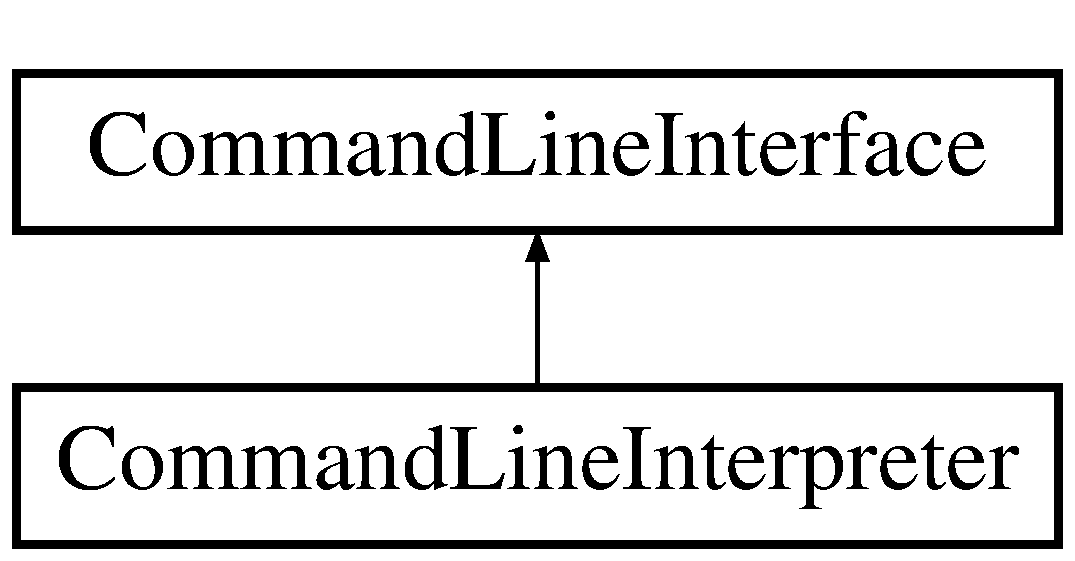
\includegraphics[height=2.000000cm]{classCommandLineInterpreter}
\end{center}
\end{figure}
\subsection*{Public Member Functions}
\begin{DoxyCompactItemize}
\item 
\hyperlink{classCommandLineInterpreter_a01f8bc835f57c535fd20b75d83825067}{Command\-Line\-Interpreter} (int argc, char $\ast$argv\mbox{[}$\,$\mbox{]})
\begin{DoxyCompactList}\small\item\em Create a new Command Line Interpreter. \end{DoxyCompactList}\item 
\hypertarget{classCommandLineInterpreter_ac47f18ba85e0a282c1e4e073aa9681e6}{bool \hyperlink{classCommandLineInterpreter_ac47f18ba85e0a282c1e4e073aa9681e6}{opt\-\_\-exist} (std\-::string key)}\label{classCommandLineInterpreter_ac47f18ba85e0a282c1e4e073aa9681e6}

\begin{DoxyCompactList}\small\item\em Does a key exist? \end{DoxyCompactList}\item 
\hypertarget{classCommandLineInterpreter_a98b3e98a2a9f6bb1df34e7c1ce438738}{std\-::string \hyperlink{classCommandLineInterpreter_a98b3e98a2a9f6bb1df34e7c1ce438738}{get\-\_\-opt} (std\-::string key)}\label{classCommandLineInterpreter_a98b3e98a2a9f6bb1df34e7c1ce438738}

\begin{DoxyCompactList}\small\item\em Get an option by key. \end{DoxyCompactList}\item 
std\-::string \hyperlink{classCommandLineInterpreter_a6d8a4dd860eca967dc27c47d06e92075}{get\-\_\-program\-\_\-name} ()
\begin{DoxyCompactList}\small\item\em Get the program name. \end{DoxyCompactList}\end{DoxyCompactItemize}


\subsection{Constructor \& Destructor Documentation}
\hypertarget{classCommandLineInterpreter_a01f8bc835f57c535fd20b75d83825067}{\index{Command\-Line\-Interpreter@{Command\-Line\-Interpreter}!Command\-Line\-Interpreter@{Command\-Line\-Interpreter}}
\index{Command\-Line\-Interpreter@{Command\-Line\-Interpreter}!CommandLineInterpreter@{Command\-Line\-Interpreter}}
\subsubsection[{Command\-Line\-Interpreter}]{\setlength{\rightskip}{0pt plus 5cm}Command\-Line\-Interpreter\-::\-Command\-Line\-Interpreter (
\begin{DoxyParamCaption}
\item[{int}]{argc, }
\item[{char $\ast$}]{argv\mbox{[}$\,$\mbox{]}}
\end{DoxyParamCaption}
)}}\label{classCommandLineInterpreter_a01f8bc835f57c535fd20b75d83825067}


Create a new Command Line Interpreter. 

Here we create a new interpreter by passing in the two arguments from the main method, int argc \& char$\ast$ argv\mbox{[}\mbox{]}. This parses arguments passed in the form\-: -\/arg\-\_\-key=arg\-\_\-val 

\subsection{Member Function Documentation}
\hypertarget{classCommandLineInterpreter_a6d8a4dd860eca967dc27c47d06e92075}{\index{Command\-Line\-Interpreter@{Command\-Line\-Interpreter}!get\-\_\-program\-\_\-name@{get\-\_\-program\-\_\-name}}
\index{get\-\_\-program\-\_\-name@{get\-\_\-program\-\_\-name}!CommandLineInterpreter@{Command\-Line\-Interpreter}}
\subsubsection[{get\-\_\-program\-\_\-name}]{\setlength{\rightskip}{0pt plus 5cm}std\-::string Command\-Line\-Interpreter\-::get\-\_\-program\-\_\-name (
\begin{DoxyParamCaption}
{}
\end{DoxyParamCaption}
)\hspace{0.3cm}{\ttfamily [inline]}, {\ttfamily [virtual]}}}\label{classCommandLineInterpreter_a6d8a4dd860eca967dc27c47d06e92075}


Get the program name. 

Get the name of the executable currently being run. 

Implements \hyperlink{classCommandLineInterface_a47bd2a11bc8d8f507a7f75dbef36a3c9}{Command\-Line\-Interface}.



The documentation for this class was generated from the following file\-:\begin{DoxyCompactItemize}
\item 
lib/include/cli.\-h\end{DoxyCompactItemize}

\hypertarget{classConsulAdmin}{\section{Consul\-Admin Class Reference}
\label{classConsulAdmin}\index{Consul\-Admin@{Consul\-Admin}}
}


The Consul Administrator, who handles distributed configuration \& service discovery.  




{\ttfamily \#include $<$consul\-\_\-admin.\-h$>$}

\subsection*{Public Member Functions}
\begin{DoxyCompactItemize}
\item 
\hypertarget{classConsulAdmin_aafb2c493da3672acc348fd865036a883}{\hyperlink{classConsulAdmin_aafb2c493da3672acc348fd865036a883}{Consul\-Admin} (std\-::string caddr)}\label{classConsulAdmin_aafb2c493da3672acc348fd865036a883}

\begin{DoxyCompactList}\small\item\em Construct a consul admin, passing in the connection string. \end{DoxyCompactList}\item 
\hypertarget{classConsulAdmin_ac84ff8c80f6bd731329c8acb6d236759}{\hyperlink{classConsulAdmin_ac84ff8c80f6bd731329c8acb6d236759}{$\sim$\-Consul\-Admin} ()}\label{classConsulAdmin_ac84ff8c80f6bd731329c8acb6d236759}

\begin{DoxyCompactList}\small\item\em Delete a consul admin. \end{DoxyCompactList}\item 
\hypertarget{classConsulAdmin_aa83d0567051f66cf014f235586b2780f}{bool \hyperlink{classConsulAdmin_aa83d0567051f66cf014f235586b2780f}{register\-\_\-service} (\hyperlink{classService}{Service} \&s)}\label{classConsulAdmin_aa83d0567051f66cf014f235586b2780f}

\begin{DoxyCompactList}\small\item\em Register the \hyperlink{classService}{Service}. \end{DoxyCompactList}\item 
\hypertarget{classConsulAdmin_ab3772ffad9c8751fd3ba909b67c9af5b}{bool \hyperlink{classConsulAdmin_ab3772ffad9c8751fd3ba909b67c9af5b}{deregister\-\_\-service} (\hyperlink{classService}{Service} \&s)}\label{classConsulAdmin_ab3772ffad9c8751fd3ba909b67c9af5b}

\begin{DoxyCompactList}\small\item\em Deregister the \hyperlink{classService}{Service}. \end{DoxyCompactList}\item 
bool \hyperlink{classConsulAdmin_a152fc37965039733bb53c56e208b4492}{set\-\_\-config\-\_\-value} (std\-::string key, std\-::string val)
\begin{DoxyCompactList}\small\item\em Set a configuration value. \end{DoxyCompactList}\item 
\hypertarget{classConsulAdmin_a42569b08fba671535856c345fa05ef33}{std\-::string \hyperlink{classConsulAdmin_a42569b08fba671535856c345fa05ef33}{get\-\_\-config\-\_\-value} (std\-::string key)}\label{classConsulAdmin_a42569b08fba671535856c345fa05ef33}

\begin{DoxyCompactList}\small\item\em Get a configuration value. \end{DoxyCompactList}\item 
\hypertarget{classConsulAdmin_a177d6d946f41c4efa8ad0746e04b3641}{bool \hyperlink{classConsulAdmin_a177d6d946f41c4efa8ad0746e04b3641}{del\-\_\-config\-\_\-value} (std\-::string key)}\label{classConsulAdmin_a177d6d946f41c4efa8ad0746e04b3641}

\begin{DoxyCompactList}\small\item\em Delete a configuration value. \end{DoxyCompactList}\item 
\hypertarget{classConsulAdmin_a0e06b8914ba53221ad7756b1afe16d00}{std\-::string \hyperlink{classConsulAdmin_a0e06b8914ba53221ad7756b1afe16d00}{services} ()}\label{classConsulAdmin_a0e06b8914ba53221ad7756b1afe16d00}

\begin{DoxyCompactList}\small\item\em Query the local agent for services registered. \end{DoxyCompactList}\item 
\hypertarget{classConsulAdmin_a815abcc0f65f0f20d27e4832d1c08994}{std\-::string \hyperlink{classConsulAdmin_a815abcc0f65f0f20d27e4832d1c08994}{agent\-\_\-info} ()}\label{classConsulAdmin_a815abcc0f65f0f20d27e4832d1c08994}

\begin{DoxyCompactList}\small\item\em Query the local agent for it's info. \end{DoxyCompactList}\item 
\hypertarget{classConsulAdmin_a65391086283846fb4056a8f84105f9bd}{std\-::string \hyperlink{classConsulAdmin_a65391086283846fb4056a8f84105f9bd}{healthy\-\_\-services} ()}\label{classConsulAdmin_a65391086283846fb4056a8f84105f9bd}

\begin{DoxyCompactList}\small\item\em Query for healthy services only. \end{DoxyCompactList}\item 
\hypertarget{classConsulAdmin_a9086263fd0d739607b30706dc86ad047}{std\-::string \hyperlink{classConsulAdmin_a9086263fd0d739607b30706dc86ad047}{datacenters} ()}\label{classConsulAdmin_a9086263fd0d739607b30706dc86ad047}

\begin{DoxyCompactList}\small\item\em Query the catalog for datacenters. \end{DoxyCompactList}\item 
\hypertarget{classConsulAdmin_a20888c98619dc9bed63ecda78085fd4a}{std\-::string \hyperlink{classConsulAdmin_a20888c98619dc9bed63ecda78085fd4a}{nodes\-\_\-dc} (std\-::string data\-\_\-center)}\label{classConsulAdmin_a20888c98619dc9bed63ecda78085fd4a}

\begin{DoxyCompactList}\small\item\em Query the catalog for the nodes in a particular datacenter. \end{DoxyCompactList}\item 
\hypertarget{classConsulAdmin_aaac11b600131ef18b5d88d51102a8007}{std\-::string \hyperlink{classConsulAdmin_aaac11b600131ef18b5d88d51102a8007}{services\-\_\-dc} (std\-::string data\-\_\-center)}\label{classConsulAdmin_aaac11b600131ef18b5d88d51102a8007}

\begin{DoxyCompactList}\small\item\em Query the catalog for the services in a particular datacenter. \end{DoxyCompactList}\item 
\hypertarget{classConsulAdmin_ad667e4ff5102614a50a0e719eccd1ea4}{std\-::string \hyperlink{classConsulAdmin_ad667e4ff5102614a50a0e719eccd1ea4}{nodes\-\_\-service} (std\-::string service)}\label{classConsulAdmin_ad667e4ff5102614a50a0e719eccd1ea4}

\begin{DoxyCompactList}\small\item\em Query the catalog for the nodes running a particular service. \end{DoxyCompactList}\item 
\hypertarget{classConsulAdmin_a42bf71278508f190a7eeb345c9c692e1}{std\-::string \hyperlink{classConsulAdmin_a42bf71278508f190a7eeb345c9c692e1}{services\-\_\-node} (std\-::string node, std\-::string data\-\_\-center)}\label{classConsulAdmin_a42bf71278508f190a7eeb345c9c692e1}

\begin{DoxyCompactList}\small\item\em Query the catalog for the services provided by a particular node. \end{DoxyCompactList}\end{DoxyCompactItemize}


\subsection{Detailed Description}
The Consul Administrator, who handles distributed configuration \& service discovery. 

This relies on the H\-T\-T\-P Administrator, and takes in a \hyperlink{classService}{Service} object in order to register. It's responses are J\-S\-O\-N strings that are recieved from Consul. Note that the values returned from the Key-\/\-Value store will be stored in base64 format 

\subsection{Member Function Documentation}
\hypertarget{classConsulAdmin_a152fc37965039733bb53c56e208b4492}{\index{Consul\-Admin@{Consul\-Admin}!set\-\_\-config\-\_\-value@{set\-\_\-config\-\_\-value}}
\index{set\-\_\-config\-\_\-value@{set\-\_\-config\-\_\-value}!ConsulAdmin@{Consul\-Admin}}
\subsubsection[{set\-\_\-config\-\_\-value}]{\setlength{\rightskip}{0pt plus 5cm}bool Consul\-Admin\-::set\-\_\-config\-\_\-value (
\begin{DoxyParamCaption}
\item[{std\-::string}]{key, }
\item[{std\-::string}]{val}
\end{DoxyParamCaption}
)}}\label{classConsulAdmin_a152fc37965039733bb53c56e208b4492}


Set a configuration value. 

If the key does not exist, then this will add it. Otherwise, it will update the existing key. 

The documentation for this class was generated from the following files\-:\begin{DoxyCompactItemize}
\item 
lib/include/consul\-\_\-admin.\-h\item 
lib/consul\-\_\-admin.\-cpp\end{DoxyCompactItemize}

\hypertarget{classConsulInterface}{}\section{Consul\+Interface Class Reference}
\label{classConsulInterface}\index{Consul\+Interface@{Consul\+Interface}}


The Consul Administrator, who handles distributed configuration \& service discovery.  




{\ttfamily \#include $<$consul\+\_\+interface.\+h$>$}

\subsection*{Public Member Functions}
\begin{DoxyCompactItemize}
\item 
virtual std\+::string \hyperlink{classConsulInterface_a636b134672f2c150f6b38fc821fb2348}{base64\+\_\+decode} (std\+::string const \&encoded\+\_\+string)=0
\begin{DoxyCompactList}\small\item\em Convinience Method for base64 decoding. \end{DoxyCompactList}\item 
virtual bool \hyperlink{classConsulInterface_ad1d3a241b2fc31e4b13789a49a0d010a}{register\+\_\+service} (\hyperlink{classServiceInterface}{Service\+Interface} \&s)=0\hypertarget{classConsulInterface_ad1d3a241b2fc31e4b13789a49a0d010a}{}\label{classConsulInterface_ad1d3a241b2fc31e4b13789a49a0d010a}

\begin{DoxyCompactList}\small\item\em Register the Service. \end{DoxyCompactList}\item 
virtual bool \hyperlink{classConsulInterface_ac97f7a426f3de5023edc637ab984b4c4}{deregister\+\_\+service} (\hyperlink{classServiceInterface}{Service\+Interface} \&s)=0\hypertarget{classConsulInterface_ac97f7a426f3de5023edc637ab984b4c4}{}\label{classConsulInterface_ac97f7a426f3de5023edc637ab984b4c4}

\begin{DoxyCompactList}\small\item\em Deregister the Service. \end{DoxyCompactList}\item 
virtual bool \hyperlink{classConsulInterface_a98ce2623db59b3f8804691a4039957a8}{set\+\_\+config\+\_\+value} (std\+::string key, std\+::string val)=0
\begin{DoxyCompactList}\small\item\em Set a configuration value. \end{DoxyCompactList}\item 
virtual std\+::string \hyperlink{classConsulInterface_a1cc4bdfe75f86f69626e109847aba6af}{get\+\_\+config\+\_\+value} (std\+::string key)=0\hypertarget{classConsulInterface_a1cc4bdfe75f86f69626e109847aba6af}{}\label{classConsulInterface_a1cc4bdfe75f86f69626e109847aba6af}

\begin{DoxyCompactList}\small\item\em Get a configuration value. \end{DoxyCompactList}\item 
virtual bool \hyperlink{classConsulInterface_a3a6e57ac45cf284e92def6136b0e23d9}{del\+\_\+config\+\_\+value} (std\+::string key)=0\hypertarget{classConsulInterface_a3a6e57ac45cf284e92def6136b0e23d9}{}\label{classConsulInterface_a3a6e57ac45cf284e92def6136b0e23d9}

\begin{DoxyCompactList}\small\item\em Delete a configuration value. \end{DoxyCompactList}\item 
virtual std\+::string \hyperlink{classConsulInterface_ad130a602282f9854a2eae856bb60a745}{services} ()=0\hypertarget{classConsulInterface_ad130a602282f9854a2eae856bb60a745}{}\label{classConsulInterface_ad130a602282f9854a2eae856bb60a745}

\begin{DoxyCompactList}\small\item\em Query the local agent for services registered. \end{DoxyCompactList}\item 
virtual std\+::string \hyperlink{classConsulInterface_a6fb0bda867b267614b44328fd044859e}{agent\+\_\+info} ()=0\hypertarget{classConsulInterface_a6fb0bda867b267614b44328fd044859e}{}\label{classConsulInterface_a6fb0bda867b267614b44328fd044859e}

\begin{DoxyCompactList}\small\item\em Query the local agent for it\textquotesingle{}s info. \end{DoxyCompactList}\item 
virtual std\+::string \hyperlink{classConsulInterface_a229eaac89811b9e1f5f3c9ec70ea68aa}{healthy\+\_\+services} ()=0\hypertarget{classConsulInterface_a229eaac89811b9e1f5f3c9ec70ea68aa}{}\label{classConsulInterface_a229eaac89811b9e1f5f3c9ec70ea68aa}

\begin{DoxyCompactList}\small\item\em Query for healthy services only. \end{DoxyCompactList}\item 
virtual std\+::string \hyperlink{classConsulInterface_a16848fcc856afae488c55e4f4febf268}{datacenters} ()=0\hypertarget{classConsulInterface_a16848fcc856afae488c55e4f4febf268}{}\label{classConsulInterface_a16848fcc856afae488c55e4f4febf268}

\begin{DoxyCompactList}\small\item\em Query the catalog for datacenters. \end{DoxyCompactList}\item 
virtual std\+::string \hyperlink{classConsulInterface_a0831246af1b80ce5bbe074a47333c615}{nodes\+\_\+dc} (std\+::string data\+\_\+center)=0\hypertarget{classConsulInterface_a0831246af1b80ce5bbe074a47333c615}{}\label{classConsulInterface_a0831246af1b80ce5bbe074a47333c615}

\begin{DoxyCompactList}\small\item\em Query the catalog for the nodes in a particular datacenter. \end{DoxyCompactList}\item 
virtual std\+::string \hyperlink{classConsulInterface_ab1c3f2169a8aebdb5a66cfe8211330dc}{services\+\_\+dc} (std\+::string data\+\_\+center)=0\hypertarget{classConsulInterface_ab1c3f2169a8aebdb5a66cfe8211330dc}{}\label{classConsulInterface_ab1c3f2169a8aebdb5a66cfe8211330dc}

\begin{DoxyCompactList}\small\item\em Query the catalog for the services in a particular datacenter. \end{DoxyCompactList}\item 
virtual std\+::string \hyperlink{classConsulInterface_a7490a960b2e10855c7d7ff09d87942b8}{nodes\+\_\+service} (std\+::string service)=0\hypertarget{classConsulInterface_a7490a960b2e10855c7d7ff09d87942b8}{}\label{classConsulInterface_a7490a960b2e10855c7d7ff09d87942b8}

\begin{DoxyCompactList}\small\item\em Query the catalog for the nodes running a particular service. \end{DoxyCompactList}\item 
virtual std\+::string \hyperlink{classConsulInterface_abbd5b2839d3548d48e93074a53844f40}{services\+\_\+node} (std\+::string node, std\+::string data\+\_\+center)=0\hypertarget{classConsulInterface_abbd5b2839d3548d48e93074a53844f40}{}\label{classConsulInterface_abbd5b2839d3548d48e93074a53844f40}

\begin{DoxyCompactList}\small\item\em Query the catalog for the services provided by a particular node. \end{DoxyCompactList}\end{DoxyCompactItemize}


\subsection{Detailed Description}
The Consul Administrator, who handles distributed configuration \& service discovery. 

This relies on the H\+T\+TP Administrator, and takes in a Service object in order to register. It\textquotesingle{}s responses are J\+S\+ON strings that are recieved from Consul. Note that the values returned from the Key-\/\+Value store will be stored in base64 format 

\subsection{Member Function Documentation}
\index{Consul\+Interface@{Consul\+Interface}!base64\+\_\+decode@{base64\+\_\+decode}}
\index{base64\+\_\+decode@{base64\+\_\+decode}!Consul\+Interface@{Consul\+Interface}}
\subsubsection[{\texorpdfstring{base64\+\_\+decode(std\+::string const \&encoded\+\_\+string)=0}{base64_decode(std::string const &encoded_string)=0}}]{\setlength{\rightskip}{0pt plus 5cm}virtual std\+::string Consul\+Interface\+::base64\+\_\+decode (
\begin{DoxyParamCaption}
\item[{std\+::string const \&}]{encoded\+\_\+string}
\end{DoxyParamCaption}
)\hspace{0.3cm}{\ttfamily [pure virtual]}}\hypertarget{classConsulInterface_a636b134672f2c150f6b38fc821fb2348}{}\label{classConsulInterface_a636b134672f2c150f6b38fc821fb2348}


Convinience Method for base64 decoding. 

This is needed as all configuration values are returned from Consul in base64, and need to be decoded after the json is parsed. \index{Consul\+Interface@{Consul\+Interface}!set\+\_\+config\+\_\+value@{set\+\_\+config\+\_\+value}}
\index{set\+\_\+config\+\_\+value@{set\+\_\+config\+\_\+value}!Consul\+Interface@{Consul\+Interface}}
\subsubsection[{\texorpdfstring{set\+\_\+config\+\_\+value(std\+::string key, std\+::string val)=0}{set_config_value(std::string key, std::string val)=0}}]{\setlength{\rightskip}{0pt plus 5cm}virtual bool Consul\+Interface\+::set\+\_\+config\+\_\+value (
\begin{DoxyParamCaption}
\item[{std\+::string}]{key, }
\item[{std\+::string}]{val}
\end{DoxyParamCaption}
)\hspace{0.3cm}{\ttfamily [pure virtual]}}\hypertarget{classConsulInterface_a98ce2623db59b3f8804691a4039957a8}{}\label{classConsulInterface_a98ce2623db59b3f8804691a4039957a8}


Set a configuration value. 

If the key does not exist, then this will add it. Otherwise, it will update the existing key. 

The documentation for this class was generated from the following file\+:\begin{DoxyCompactItemize}
\item 
aossl/consul/include/consul\+\_\+interface.\+h\end{DoxyCompactItemize}

\hypertarget{classCouchbaseAdmin}{\section{Couchbase\-Admin Class Reference}
\label{classCouchbaseAdmin}\index{Couchbase\-Admin@{Couchbase\-Admin}}
}


The Couchbase Administrator handles interactions with the Couchbase D\-B.  




{\ttfamily \#include $<$couchbase\-\_\-admin.\-h$>$}

Inheritance diagram for Couchbase\-Admin\-:\begin{figure}[H]
\begin{center}
\leavevmode
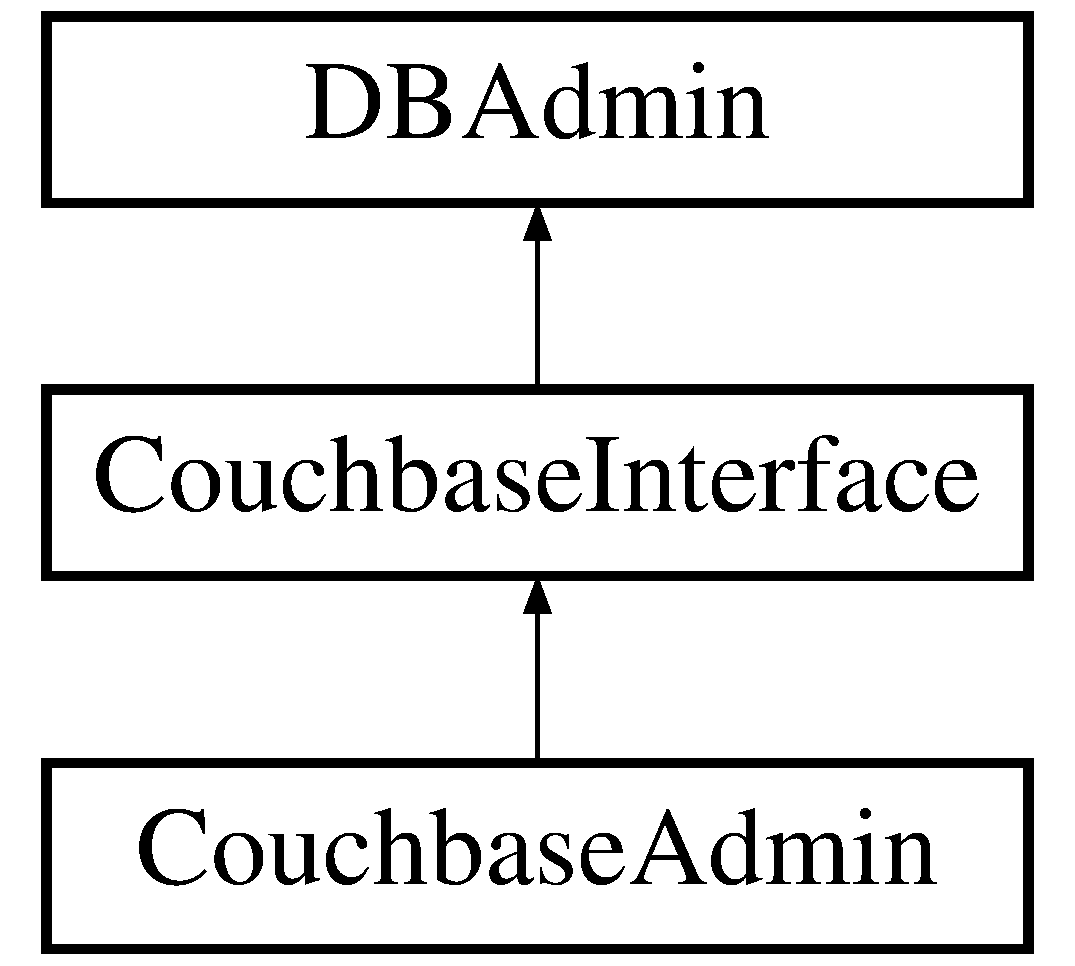
\includegraphics[height=2.000000cm]{classCouchbaseAdmin}
\end{center}
\end{figure}
\subsection*{Public Member Functions}
\begin{DoxyCompactItemize}
\item 
\hypertarget{classCouchbaseAdmin_a4a92b5209d65af9c9166b2fcb7aa6f07}{\hyperlink{classCouchbaseAdmin_a4a92b5209d65af9c9166b2fcb7aa6f07}{Couchbase\-Admin} (const char $\ast$conn)}\label{classCouchbaseAdmin_a4a92b5209d65af9c9166b2fcb7aa6f07}

\begin{DoxyCompactList}\small\item\em Create a new Couchbase Admin, without a password. \end{DoxyCompactList}\item 
\hypertarget{classCouchbaseAdmin_ab0ef48f5376cb28ddbd1a23f139ecb04}{\hyperlink{classCouchbaseAdmin_ab0ef48f5376cb28ddbd1a23f139ecb04}{Couchbase\-Admin} (const char $\ast$conn, const char $\ast$pswd)}\label{classCouchbaseAdmin_ab0ef48f5376cb28ddbd1a23f139ecb04}

\begin{DoxyCompactList}\small\item\em Create a new Couchbase Admin, with a password. \end{DoxyCompactList}\item 
\hypertarget{classCouchbaseAdmin_a1e762f3c30cf9e855258911d2f642a07}{\hyperlink{classCouchbaseAdmin_a1e762f3c30cf9e855258911d2f642a07}{$\sim$\-Couchbase\-Admin} ()}\label{classCouchbaseAdmin_a1e762f3c30cf9e855258911d2f642a07}

\begin{DoxyCompactList}\small\item\em Delete the Couchbase Admin. \end{DoxyCompactList}\item 
void \hyperlink{classCouchbaseAdmin_afc05e9ffcd5fa9dd557cbd452b1d91db}{load\-\_\-object} (const char $\ast$key)
\begin{DoxyCompactList}\small\item\em Load a J\-S\-O\-N Object from the Couchbase D\-B. \end{DoxyCompactList}\item 
void \hyperlink{classCouchbaseAdmin_a88a4592398aba43761a3a43873f012db}{save\-\_\-object} (\hyperlink{classWriteable}{Writeable} $\ast$obj)
\begin{DoxyCompactList}\small\item\em Save a J\-S\-O\-N Object to the Couchbase D\-B. \end{DoxyCompactList}\item 
void \hyperlink{classCouchbaseAdmin_af2a2f49b4085db2493c6c72db9143060}{create\-\_\-object} (\hyperlink{classWriteable}{Writeable} $\ast$obj)
\begin{DoxyCompactList}\small\item\em Create a J\-S\-O\-N Object in the Couchbase D\-B. \end{DoxyCompactList}\item 
void \hyperlink{classCouchbaseAdmin_a7304d9e45d68415042e8f097a90d39f1}{delete\-\_\-object} (const char $\ast$key)
\begin{DoxyCompactList}\small\item\em Delete a J\-S\-O\-N Object from the Couchbase D\-B. \end{DoxyCompactList}\item 
void \hyperlink{classCouchbaseAdmin_a5ee5a510733d51a72df3d3e64419e35a}{bind\-\_\-get\-\_\-callback} (Get\-Callback)
\begin{DoxyCompactList}\small\item\em Bind the Retrieval Callback. \end{DoxyCompactList}\item 
void \hyperlink{classCouchbaseAdmin_a38ab8dcaa03d56c822705560e39bf199}{bind\-\_\-storage\-\_\-callback} (Storage\-Callback)
\begin{DoxyCompactList}\small\item\em Bind the Storage Callback. \end{DoxyCompactList}\item 
void \hyperlink{classCouchbaseAdmin_a4effd1e925f32d2a1bb08401ab14ad07}{bind\-\_\-delete\-\_\-callback} (Del\-Callback)
\begin{DoxyCompactList}\small\item\em Bind the Removal Callback. \end{DoxyCompactList}\item 
\hypertarget{classCouchbaseAdmin_ad5f13695bc2ff678699a7afc9122d043}{lcb\-\_\-t \hyperlink{classCouchbaseAdmin_ad5f13695bc2ff678699a7afc9122d043}{get\-\_\-instance} ()}\label{classCouchbaseAdmin_ad5f13695bc2ff678699a7afc9122d043}

\begin{DoxyCompactList}\small\item\em Get the instance, for advanced operations if necessary. Not advised. \end{DoxyCompactList}\item 
\hypertarget{classCouchbaseAdmin_a8a59b17e86597f311103a26d4b0fef61}{void \hyperlink{classCouchbaseAdmin_a8a59b17e86597f311103a26d4b0fef61}{wait} ()}\label{classCouchbaseAdmin_a8a59b17e86597f311103a26d4b0fef61}

\begin{DoxyCompactList}\small\item\em Blocking call until the transaction stack is empty. \end{DoxyCompactList}\end{DoxyCompactItemize}


\subsection{Detailed Description}
The Couchbase Administrator handles interactions with the Couchbase D\-B. 

This binds a number of callbacks for major operations, and supports full C\-R\-U\-D operations on J\-S\-O\-N documents stored in the Couchbase D\-B 

\subsection{Member Function Documentation}
\hypertarget{classCouchbaseAdmin_a4effd1e925f32d2a1bb08401ab14ad07}{\index{Couchbase\-Admin@{Couchbase\-Admin}!bind\-\_\-delete\-\_\-callback@{bind\-\_\-delete\-\_\-callback}}
\index{bind\-\_\-delete\-\_\-callback@{bind\-\_\-delete\-\_\-callback}!CouchbaseAdmin@{Couchbase\-Admin}}
\subsubsection[{bind\-\_\-delete\-\_\-callback}]{\setlength{\rightskip}{0pt plus 5cm}void Couchbase\-Admin\-::bind\-\_\-delete\-\_\-callback (
\begin{DoxyParamCaption}
\item[{Del\-Callback}]{dc}
\end{DoxyParamCaption}
)}}\label{classCouchbaseAdmin_a4effd1e925f32d2a1bb08401ab14ad07}


Bind the Removal Callback. 

When the requested object is deleted, the method bound with bind\-\_\-delete\-\_\-callback will be executed \hypertarget{classCouchbaseAdmin_a5ee5a510733d51a72df3d3e64419e35a}{\index{Couchbase\-Admin@{Couchbase\-Admin}!bind\-\_\-get\-\_\-callback@{bind\-\_\-get\-\_\-callback}}
\index{bind\-\_\-get\-\_\-callback@{bind\-\_\-get\-\_\-callback}!CouchbaseAdmin@{Couchbase\-Admin}}
\subsubsection[{bind\-\_\-get\-\_\-callback}]{\setlength{\rightskip}{0pt plus 5cm}void Couchbase\-Admin\-::bind\-\_\-get\-\_\-callback (
\begin{DoxyParamCaption}
\item[{Get\-Callback}]{gc}
\end{DoxyParamCaption}
)}}\label{classCouchbaseAdmin_a5ee5a510733d51a72df3d3e64419e35a}


Bind the Retrieval Callback. 

When the requested object is loaded, the method bound with bind\-\_\-get\-\_\-callback will be executed \hypertarget{classCouchbaseAdmin_a38ab8dcaa03d56c822705560e39bf199}{\index{Couchbase\-Admin@{Couchbase\-Admin}!bind\-\_\-storage\-\_\-callback@{bind\-\_\-storage\-\_\-callback}}
\index{bind\-\_\-storage\-\_\-callback@{bind\-\_\-storage\-\_\-callback}!CouchbaseAdmin@{Couchbase\-Admin}}
\subsubsection[{bind\-\_\-storage\-\_\-callback}]{\setlength{\rightskip}{0pt plus 5cm}void Couchbase\-Admin\-::bind\-\_\-storage\-\_\-callback (
\begin{DoxyParamCaption}
\item[{Storage\-Callback}]{sc}
\end{DoxyParamCaption}
)}}\label{classCouchbaseAdmin_a38ab8dcaa03d56c822705560e39bf199}


Bind the Storage Callback. 

When the requested object is saved or created, the method bound with bind\-\_\-storage\-\_\-callback will be executed \hypertarget{classCouchbaseAdmin_af2a2f49b4085db2493c6c72db9143060}{\index{Couchbase\-Admin@{Couchbase\-Admin}!create\-\_\-object@{create\-\_\-object}}
\index{create\-\_\-object@{create\-\_\-object}!CouchbaseAdmin@{Couchbase\-Admin}}
\subsubsection[{create\-\_\-object}]{\setlength{\rightskip}{0pt plus 5cm}void Couchbase\-Admin\-::create\-\_\-object (
\begin{DoxyParamCaption}
\item[{{\bf Writeable} $\ast$}]{obj}
\end{DoxyParamCaption}
)\hspace{0.3cm}{\ttfamily [virtual]}}}\label{classCouchbaseAdmin_af2a2f49b4085db2493c6c72db9143060}


Create a J\-S\-O\-N Object in the Couchbase D\-B. 

The requested object is saved and, when complete, the method bound with bind\-\_\-storage\-\_\-callback will be executed 

Implements \hyperlink{classDBAdmin_aa8915761b88c5ef2df51171ff425c963}{D\-B\-Admin}.

\hypertarget{classCouchbaseAdmin_a7304d9e45d68415042e8f097a90d39f1}{\index{Couchbase\-Admin@{Couchbase\-Admin}!delete\-\_\-object@{delete\-\_\-object}}
\index{delete\-\_\-object@{delete\-\_\-object}!CouchbaseAdmin@{Couchbase\-Admin}}
\subsubsection[{delete\-\_\-object}]{\setlength{\rightskip}{0pt plus 5cm}void Couchbase\-Admin\-::delete\-\_\-object (
\begin{DoxyParamCaption}
\item[{const char $\ast$}]{key}
\end{DoxyParamCaption}
)\hspace{0.3cm}{\ttfamily [virtual]}}}\label{classCouchbaseAdmin_a7304d9e45d68415042e8f097a90d39f1}


Delete a J\-S\-O\-N Object from the Couchbase D\-B. 

The requested object is deleted and, when complete, the method bound with bind\-\_\-delete\-\_\-callback will be executed 

Implements \hyperlink{classDBAdmin_a6fffd56ad4f9db9cd951a91ecb41373b}{D\-B\-Admin}.

\hypertarget{classCouchbaseAdmin_afc05e9ffcd5fa9dd557cbd452b1d91db}{\index{Couchbase\-Admin@{Couchbase\-Admin}!load\-\_\-object@{load\-\_\-object}}
\index{load\-\_\-object@{load\-\_\-object}!CouchbaseAdmin@{Couchbase\-Admin}}
\subsubsection[{load\-\_\-object}]{\setlength{\rightskip}{0pt plus 5cm}void Couchbase\-Admin\-::load\-\_\-object (
\begin{DoxyParamCaption}
\item[{const char $\ast$}]{key}
\end{DoxyParamCaption}
)\hspace{0.3cm}{\ttfamily [virtual]}}}\label{classCouchbaseAdmin_afc05e9ffcd5fa9dd557cbd452b1d91db}


Load a J\-S\-O\-N Object from the Couchbase D\-B. 

The requested object is loaded and, when ready, the method bound with bind\-\_\-get\-\_\-callback will be executed 

Implements \hyperlink{classDBAdmin_a48ebd30b2e5bb44d23359baa86fe42b9}{D\-B\-Admin}.

\hypertarget{classCouchbaseAdmin_a88a4592398aba43761a3a43873f012db}{\index{Couchbase\-Admin@{Couchbase\-Admin}!save\-\_\-object@{save\-\_\-object}}
\index{save\-\_\-object@{save\-\_\-object}!CouchbaseAdmin@{Couchbase\-Admin}}
\subsubsection[{save\-\_\-object}]{\setlength{\rightskip}{0pt plus 5cm}void Couchbase\-Admin\-::save\-\_\-object (
\begin{DoxyParamCaption}
\item[{{\bf Writeable} $\ast$}]{obj}
\end{DoxyParamCaption}
)\hspace{0.3cm}{\ttfamily [virtual]}}}\label{classCouchbaseAdmin_a88a4592398aba43761a3a43873f012db}


Save a J\-S\-O\-N Object to the Couchbase D\-B. 

The requested object is saved and, when complete, the method bound with bind\-\_\-storage\-\_\-callback will be executed 

Implements \hyperlink{classDBAdmin_a29372700a0be4c34ef7ffb956927d9cd}{D\-B\-Admin}.



The documentation for this class was generated from the following files\-:\begin{DoxyCompactItemize}
\item 
lib/include/couchbase\-\_\-admin.\-h\item 
lib/couchbase\-\_\-admin.\-cpp\end{DoxyCompactItemize}

\hypertarget{classCouchbaseInterface}{\section{Couchbase\-Interface Class Reference}
\label{classCouchbaseInterface}\index{Couchbase\-Interface@{Couchbase\-Interface}}
}


The Couchbase Administrator handles interactions with the Couchbase D\-B.  




{\ttfamily \#include $<$couchbase\-\_\-interface.\-h$>$}

Inheritance diagram for Couchbase\-Interface\-:\begin{figure}[H]
\begin{center}
\leavevmode
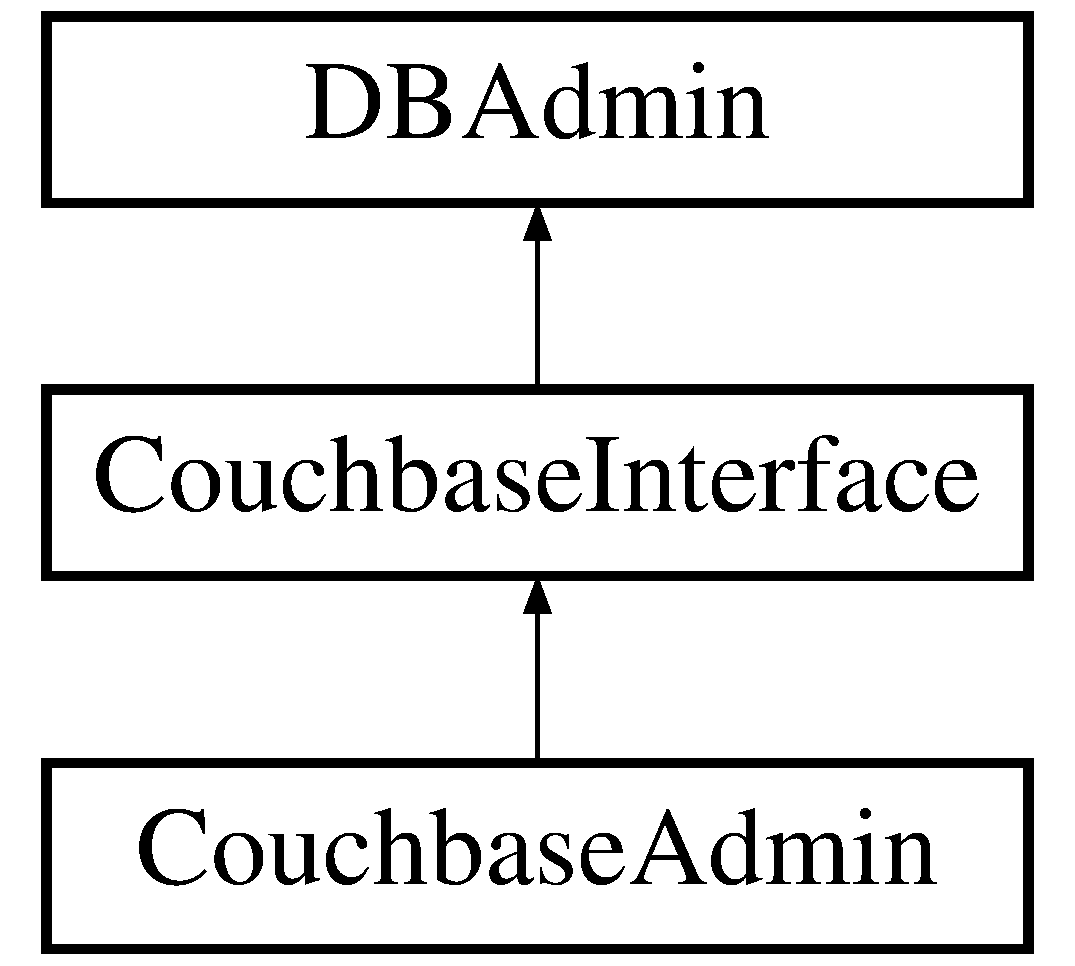
\includegraphics[height=2.000000cm]{classCouchbaseInterface}
\end{center}
\end{figure}
\subsection*{Public Member Functions}
\begin{DoxyCompactItemize}
\item 
virtual void \hyperlink{classCouchbaseInterface_a62a765de48bfc92d748df829ca960ff2}{load\-\_\-object} (const char $\ast$key)=0
\begin{DoxyCompactList}\small\item\em Load a J\-S\-O\-N Object from the Couchbase D\-B. \end{DoxyCompactList}\item 
virtual void \hyperlink{classCouchbaseInterface_ab4ea907f469d14323e451ffdccb213c2}{save\-\_\-object} (\hyperlink{classWriteable}{Writeable} $\ast$obj)=0
\begin{DoxyCompactList}\small\item\em Save a J\-S\-O\-N Object to the Couchbase D\-B. \end{DoxyCompactList}\item 
virtual void \hyperlink{classCouchbaseInterface_a7ac9545e6f7a45d24e8e41ccae1f6112}{create\-\_\-object} (\hyperlink{classWriteable}{Writeable} $\ast$obj)=0
\begin{DoxyCompactList}\small\item\em Create a J\-S\-O\-N Object in the Couchbase D\-B. \end{DoxyCompactList}\item 
virtual void \hyperlink{classCouchbaseInterface_a99ec66952f649bb84c80b20487e82839}{delete\-\_\-object} (const char $\ast$key)=0
\begin{DoxyCompactList}\small\item\em Delete a J\-S\-O\-N Object from the Couchbase D\-B. \end{DoxyCompactList}\item 
virtual void \hyperlink{classCouchbaseInterface_aea02cefeae5b210318471696bd6580c9}{bind\-\_\-get\-\_\-callback} (Get\-Callback)=0
\begin{DoxyCompactList}\small\item\em Bind the Retrieval Callback. \end{DoxyCompactList}\item 
virtual void \hyperlink{classCouchbaseInterface_a229805a21e8dec6d5a4636644b420996}{bind\-\_\-storage\-\_\-callback} (Storage\-Callback)=0
\begin{DoxyCompactList}\small\item\em Bind the Storage Callback. \end{DoxyCompactList}\item 
virtual void \hyperlink{classCouchbaseInterface_a58fc6806bf33bc98c25d943fa1809505}{bind\-\_\-delete\-\_\-callback} (Del\-Callback)=0
\begin{DoxyCompactList}\small\item\em Bind the Removal Callback. \end{DoxyCompactList}\item 
\hypertarget{classCouchbaseInterface_ae901a3e383a82044679d0b77702c7e2c}{virtual void \hyperlink{classCouchbaseInterface_ae901a3e383a82044679d0b77702c7e2c}{wait} ()=0}\label{classCouchbaseInterface_ae901a3e383a82044679d0b77702c7e2c}

\begin{DoxyCompactList}\small\item\em Blocking call until the transaction stack is empty. \end{DoxyCompactList}\end{DoxyCompactItemize}


\subsection{Detailed Description}
The Couchbase Administrator handles interactions with the Couchbase D\-B. 

This binds a number of callbacks for major operations, and supports full C\-R\-U\-D operations on J\-S\-O\-N documents stored in the Couchbase D\-B 

\subsection{Member Function Documentation}
\hypertarget{classCouchbaseInterface_a58fc6806bf33bc98c25d943fa1809505}{\index{Couchbase\-Interface@{Couchbase\-Interface}!bind\-\_\-delete\-\_\-callback@{bind\-\_\-delete\-\_\-callback}}
\index{bind\-\_\-delete\-\_\-callback@{bind\-\_\-delete\-\_\-callback}!CouchbaseInterface@{Couchbase\-Interface}}
\subsubsection[{bind\-\_\-delete\-\_\-callback}]{\setlength{\rightskip}{0pt plus 5cm}virtual void Couchbase\-Interface\-::bind\-\_\-delete\-\_\-callback (
\begin{DoxyParamCaption}
\item[{Del\-Callback}]{}
\end{DoxyParamCaption}
)\hspace{0.3cm}{\ttfamily [pure virtual]}}}\label{classCouchbaseInterface_a58fc6806bf33bc98c25d943fa1809505}


Bind the Removal Callback. 

When the requested object is deleted, the method bound with bind\-\_\-delete\-\_\-callback will be executed \hypertarget{classCouchbaseInterface_aea02cefeae5b210318471696bd6580c9}{\index{Couchbase\-Interface@{Couchbase\-Interface}!bind\-\_\-get\-\_\-callback@{bind\-\_\-get\-\_\-callback}}
\index{bind\-\_\-get\-\_\-callback@{bind\-\_\-get\-\_\-callback}!CouchbaseInterface@{Couchbase\-Interface}}
\subsubsection[{bind\-\_\-get\-\_\-callback}]{\setlength{\rightskip}{0pt plus 5cm}virtual void Couchbase\-Interface\-::bind\-\_\-get\-\_\-callback (
\begin{DoxyParamCaption}
\item[{Get\-Callback}]{}
\end{DoxyParamCaption}
)\hspace{0.3cm}{\ttfamily [pure virtual]}}}\label{classCouchbaseInterface_aea02cefeae5b210318471696bd6580c9}


Bind the Retrieval Callback. 

When the requested object is loaded, the method bound with bind\-\_\-get\-\_\-callback will be executed \hypertarget{classCouchbaseInterface_a229805a21e8dec6d5a4636644b420996}{\index{Couchbase\-Interface@{Couchbase\-Interface}!bind\-\_\-storage\-\_\-callback@{bind\-\_\-storage\-\_\-callback}}
\index{bind\-\_\-storage\-\_\-callback@{bind\-\_\-storage\-\_\-callback}!CouchbaseInterface@{Couchbase\-Interface}}
\subsubsection[{bind\-\_\-storage\-\_\-callback}]{\setlength{\rightskip}{0pt plus 5cm}virtual void Couchbase\-Interface\-::bind\-\_\-storage\-\_\-callback (
\begin{DoxyParamCaption}
\item[{Storage\-Callback}]{}
\end{DoxyParamCaption}
)\hspace{0.3cm}{\ttfamily [pure virtual]}}}\label{classCouchbaseInterface_a229805a21e8dec6d5a4636644b420996}


Bind the Storage Callback. 

When the requested object is saved or created, the method bound with bind\-\_\-storage\-\_\-callback will be executed \hypertarget{classCouchbaseInterface_a7ac9545e6f7a45d24e8e41ccae1f6112}{\index{Couchbase\-Interface@{Couchbase\-Interface}!create\-\_\-object@{create\-\_\-object}}
\index{create\-\_\-object@{create\-\_\-object}!CouchbaseInterface@{Couchbase\-Interface}}
\subsubsection[{create\-\_\-object}]{\setlength{\rightskip}{0pt plus 5cm}virtual void Couchbase\-Interface\-::create\-\_\-object (
\begin{DoxyParamCaption}
\item[{{\bf Writeable} $\ast$}]{obj}
\end{DoxyParamCaption}
)\hspace{0.3cm}{\ttfamily [pure virtual]}}}\label{classCouchbaseInterface_a7ac9545e6f7a45d24e8e41ccae1f6112}


Create a J\-S\-O\-N Object in the Couchbase D\-B. 

The requested object is saved and, when complete, the method bound with bind\-\_\-storage\-\_\-callback will be executed 

Implements \hyperlink{classDBAdmin_aa8915761b88c5ef2df51171ff425c963}{D\-B\-Admin}.

\hypertarget{classCouchbaseInterface_a99ec66952f649bb84c80b20487e82839}{\index{Couchbase\-Interface@{Couchbase\-Interface}!delete\-\_\-object@{delete\-\_\-object}}
\index{delete\-\_\-object@{delete\-\_\-object}!CouchbaseInterface@{Couchbase\-Interface}}
\subsubsection[{delete\-\_\-object}]{\setlength{\rightskip}{0pt plus 5cm}virtual void Couchbase\-Interface\-::delete\-\_\-object (
\begin{DoxyParamCaption}
\item[{const char $\ast$}]{key}
\end{DoxyParamCaption}
)\hspace{0.3cm}{\ttfamily [pure virtual]}}}\label{classCouchbaseInterface_a99ec66952f649bb84c80b20487e82839}


Delete a J\-S\-O\-N Object from the Couchbase D\-B. 

The requested object is deleted and, when complete, the method bound with bind\-\_\-delete\-\_\-callback will be executed 

Implements \hyperlink{classDBAdmin_a6fffd56ad4f9db9cd951a91ecb41373b}{D\-B\-Admin}.

\hypertarget{classCouchbaseInterface_a62a765de48bfc92d748df829ca960ff2}{\index{Couchbase\-Interface@{Couchbase\-Interface}!load\-\_\-object@{load\-\_\-object}}
\index{load\-\_\-object@{load\-\_\-object}!CouchbaseInterface@{Couchbase\-Interface}}
\subsubsection[{load\-\_\-object}]{\setlength{\rightskip}{0pt plus 5cm}virtual void Couchbase\-Interface\-::load\-\_\-object (
\begin{DoxyParamCaption}
\item[{const char $\ast$}]{key}
\end{DoxyParamCaption}
)\hspace{0.3cm}{\ttfamily [pure virtual]}}}\label{classCouchbaseInterface_a62a765de48bfc92d748df829ca960ff2}


Load a J\-S\-O\-N Object from the Couchbase D\-B. 

The requested object is loaded and, when ready, the method bound with bind\-\_\-get\-\_\-callback will be executed 

Implements \hyperlink{classDBAdmin_a48ebd30b2e5bb44d23359baa86fe42b9}{D\-B\-Admin}.

\hypertarget{classCouchbaseInterface_ab4ea907f469d14323e451ffdccb213c2}{\index{Couchbase\-Interface@{Couchbase\-Interface}!save\-\_\-object@{save\-\_\-object}}
\index{save\-\_\-object@{save\-\_\-object}!CouchbaseInterface@{Couchbase\-Interface}}
\subsubsection[{save\-\_\-object}]{\setlength{\rightskip}{0pt plus 5cm}virtual void Couchbase\-Interface\-::save\-\_\-object (
\begin{DoxyParamCaption}
\item[{{\bf Writeable} $\ast$}]{obj}
\end{DoxyParamCaption}
)\hspace{0.3cm}{\ttfamily [pure virtual]}}}\label{classCouchbaseInterface_ab4ea907f469d14323e451ffdccb213c2}


Save a J\-S\-O\-N Object to the Couchbase D\-B. 

The requested object is saved and, when complete, the method bound with bind\-\_\-storage\-\_\-callback will be executed 

Implements \hyperlink{classDBAdmin_a29372700a0be4c34ef7ffb956927d9cd}{D\-B\-Admin}.



The documentation for this class was generated from the following file\-:\begin{DoxyCompactItemize}
\item 
lib/include/factory/couchbase\-\_\-interface.\-h\end{DoxyCompactItemize}

\hypertarget{classDBAdmin}{\section{D\-B\-Admin Class Reference}
\label{classDBAdmin}\index{D\-B\-Admin@{D\-B\-Admin}}
}


Database Administrator Interface.  




{\ttfamily \#include $<$db\-\_\-admin.\-h$>$}

Inheritance diagram for D\-B\-Admin\-:\begin{figure}[H]
\begin{center}
\leavevmode
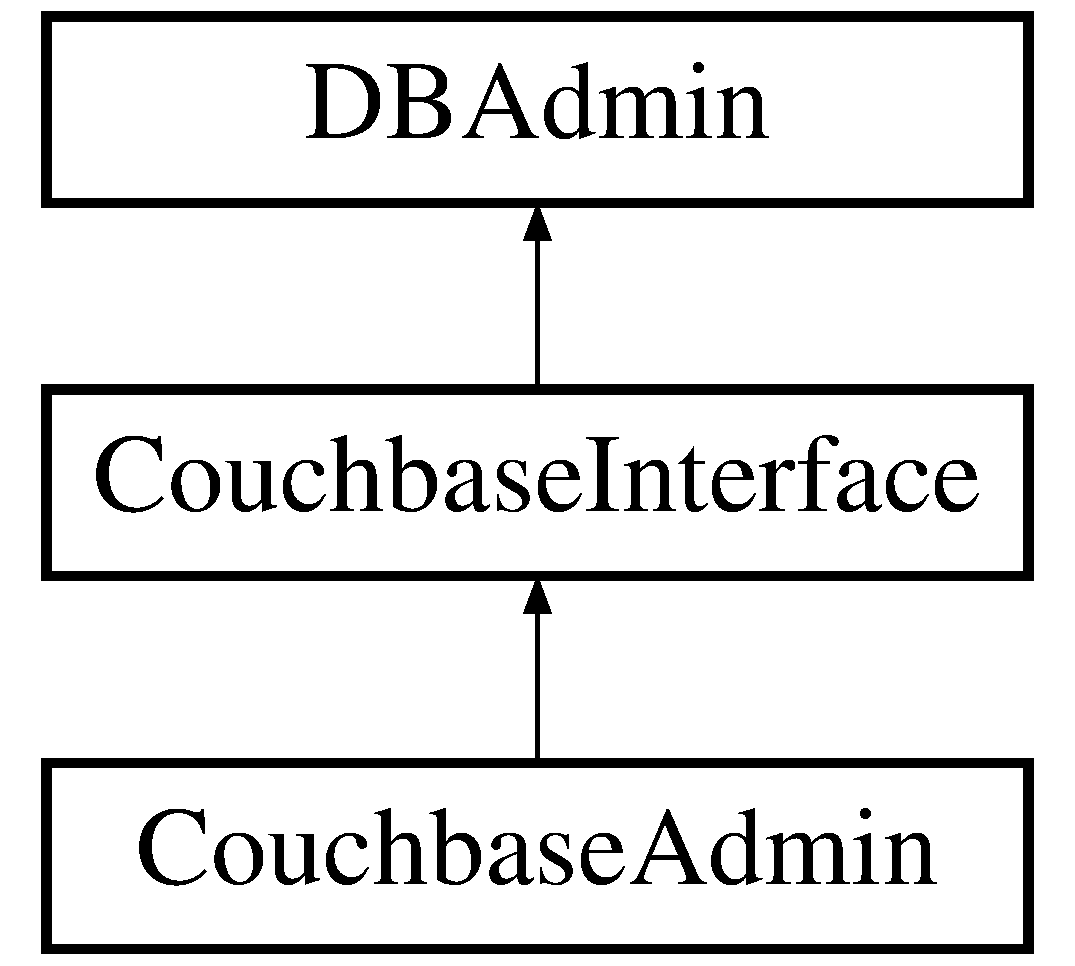
\includegraphics[height=2.000000cm]{classDBAdmin}
\end{center}
\end{figure}
\subsection*{Public Member Functions}
\begin{DoxyCompactItemize}
\item 
\hypertarget{classDBAdmin_a48ebd30b2e5bb44d23359baa86fe42b9}{virtual void \hyperlink{classDBAdmin_a48ebd30b2e5bb44d23359baa86fe42b9}{load\-\_\-object} (const char $\ast$key)=0}\label{classDBAdmin_a48ebd30b2e5bb44d23359baa86fe42b9}

\begin{DoxyCompactList}\small\item\em Load a J\-S\-O\-N Object from the D\-B. \end{DoxyCompactList}\item 
\hypertarget{classDBAdmin_a29372700a0be4c34ef7ffb956927d9cd}{virtual void \hyperlink{classDBAdmin_a29372700a0be4c34ef7ffb956927d9cd}{save\-\_\-object} (\hyperlink{classWriteable}{Writeable} $\ast$obj)=0}\label{classDBAdmin_a29372700a0be4c34ef7ffb956927d9cd}

\begin{DoxyCompactList}\small\item\em Save a J\-S\-O\-N Object to the D\-B. \end{DoxyCompactList}\item 
\hypertarget{classDBAdmin_aa8915761b88c5ef2df51171ff425c963}{virtual void \hyperlink{classDBAdmin_aa8915761b88c5ef2df51171ff425c963}{create\-\_\-object} (\hyperlink{classWriteable}{Writeable} $\ast$obj)=0}\label{classDBAdmin_aa8915761b88c5ef2df51171ff425c963}

\begin{DoxyCompactList}\small\item\em Create a J\-S\-O\-N Object in the D\-B. \end{DoxyCompactList}\item 
\hypertarget{classDBAdmin_a6fffd56ad4f9db9cd951a91ecb41373b}{virtual void \hyperlink{classDBAdmin_a6fffd56ad4f9db9cd951a91ecb41373b}{delete\-\_\-object} (const char $\ast$key)=0}\label{classDBAdmin_a6fffd56ad4f9db9cd951a91ecb41373b}

\begin{DoxyCompactList}\small\item\em Delete a J\-S\-O\-N Object from the D\-B. \end{DoxyCompactList}\item 
virtual void \hyperlink{classDBAdmin_a9a3ac4ee0b0c6453120fca46e126efe2}{wait} ()=0
\end{DoxyCompactItemize}


\subsection{Detailed Description}
Database Administrator Interface. 

An Interface defining the behavior of different Document-\/based Data Base Administrators 

\subsection{Member Function Documentation}
\hypertarget{classDBAdmin_a9a3ac4ee0b0c6453120fca46e126efe2}{\index{D\-B\-Admin@{D\-B\-Admin}!wait@{wait}}
\index{wait@{wait}!DBAdmin@{D\-B\-Admin}}
\subsubsection[{wait}]{\setlength{\rightskip}{0pt plus 5cm}virtual void D\-B\-Admin\-::wait (
\begin{DoxyParamCaption}
{}
\end{DoxyParamCaption}
)\hspace{0.3cm}{\ttfamily [pure virtual]}}}\label{classDBAdmin_a9a3ac4ee0b0c6453120fca46e126efe2}
If the engine is asynchronous, wait for the active threads to complete. Otherwise, do nothing 

Implemented in \hyperlink{classCouchbaseInterface_ae901a3e383a82044679d0b77702c7e2c}{Couchbase\-Interface}.



The documentation for this class was generated from the following file\-:\begin{DoxyCompactItemize}
\item 
lib/include/factory/db\-\_\-admin.\-h\end{DoxyCompactItemize}

\hypertarget{structHealthCheck}{}\section{Health\+Check Struct Reference}
\label{structHealthCheck}\index{Health\+Check@{Health\+Check}}


A struct to hold health check information which can be added to a service.  




{\ttfamily \#include $<$consul\+\_\+interface.\+h$>$}

\subsection*{Public Attributes}
\begin{DoxyCompactItemize}
\item 
std\+::string \hyperlink{structHealthCheck_af2cf9613abcc567941f8a21cd8c15bff}{script}\hypertarget{structHealthCheck_af2cf9613abcc567941f8a21cd8c15bff}{}\label{structHealthCheck_af2cf9613abcc567941f8a21cd8c15bff}

\begin{DoxyCompactList}\small\item\em The script to run for the health check. \end{DoxyCompactList}\item 
std\+::string \hyperlink{structHealthCheck_af8e93405495e1733ba69a7e3f73a139a}{interval}\hypertarget{structHealthCheck_af8e93405495e1733ba69a7e3f73a139a}{}\label{structHealthCheck_af8e93405495e1733ba69a7e3f73a139a}

\begin{DoxyCompactList}\small\item\em The interval for the health check. \end{DoxyCompactList}\end{DoxyCompactItemize}


\subsection{Detailed Description}
A struct to hold health check information which can be added to a service. 

The documentation for this struct was generated from the following file\+:\begin{DoxyCompactItemize}
\item 
aossl/consul/include/consul\+\_\+interface.\+h\end{DoxyCompactItemize}

\hypertarget{classHttpAdmin}{\section{Http\-Admin Class Reference}
\label{classHttpAdmin}\index{Http\-Admin@{Http\-Admin}}
}


The H\-T\-T\-P Requests Administrators.  




{\ttfamily \#include $<$http\-\_\-admin.\-h$>$}

\subsection*{Public Member Functions}
\begin{DoxyCompactItemize}
\item 
\hypertarget{classHttpAdmin_ad5821eb1e159cfad6e9e0676b8d1bd8d}{\hyperlink{classHttpAdmin_ad5821eb1e159cfad6e9e0676b8d1bd8d}{Http\-Admin} ()}\label{classHttpAdmin_ad5821eb1e159cfad6e9e0676b8d1bd8d}

\begin{DoxyCompactList}\small\item\em Start a new H\-T\-T\-P Requests Admin. \end{DoxyCompactList}\item 
\hypertarget{classHttpAdmin_acebe3cde5a43db8dd67fa47b71c37996}{void \hyperlink{classHttpAdmin_acebe3cde5a43db8dd67fa47b71c37996}{shutdown} ()}\label{classHttpAdmin_acebe3cde5a43db8dd67fa47b71c37996}

\begin{DoxyCompactList}\small\item\em Shutdown the admin. \end{DoxyCompactList}\item 
\hypertarget{classHttpAdmin_a8342985fecdaffdf72ee3a6f767236a7}{void \hyperlink{classHttpAdmin_a8342985fecdaffdf72ee3a6f767236a7}{bind\-\_\-get\-\_\-callback} (Write\-Callback)}\label{classHttpAdmin_a8342985fecdaffdf72ee3a6f767236a7}

\begin{DoxyCompactList}\small\item\em Bind Callback. \end{DoxyCompactList}\item 
\hypertarget{classHttpAdmin_abb47ebccfb59e2f11dac994d5c44fe7e}{C\-U\-R\-L $\ast$ \hyperlink{classHttpAdmin_abb47ebccfb59e2f11dac994d5c44fe7e}{get\-\_\-instance} ()}\label{classHttpAdmin_abb47ebccfb59e2f11dac994d5c44fe7e}

\begin{DoxyCompactList}\small\item\em Return the instance to bind callbacks against. Not advised. \end{DoxyCompactList}\item 
bool \hyperlink{classHttpAdmin_a671cbab4092d7602813722185560c6c4}{put} (char $\ast$url, char $\ast$data, int timeout)
\begin{DoxyCompactList}\small\item\em Put. \end{DoxyCompactList}\item 
bool \hyperlink{classHttpAdmin_a70b93e959d2cef3fe2526d78203d5b19}{get} (char $\ast$url, int timeout)
\begin{DoxyCompactList}\small\item\em Get. \end{DoxyCompactList}\item 
bool \hyperlink{classHttpAdmin_a1e323e24e18a80d635450fa218bd0025}{post} (char $\ast$url, char $\ast$data, int timeout)
\begin{DoxyCompactList}\small\item\em Post. \end{DoxyCompactList}\item 
bool \hyperlink{classHttpAdmin_ac503bfdb6ddbcb197390b57029411f8a}{del} (char $\ast$url, int timeout)
\begin{DoxyCompactList}\small\item\em Delete. \end{DoxyCompactList}\end{DoxyCompactItemize}


\subsection{Detailed Description}
The H\-T\-T\-P Requests Administrators. 

This class is in charge of making H\-T\-T\-P Requests Support for put, get post, and delete 

\subsection{Member Function Documentation}
\hypertarget{classHttpAdmin_ac503bfdb6ddbcb197390b57029411f8a}{\index{Http\-Admin@{Http\-Admin}!del@{del}}
\index{del@{del}!HttpAdmin@{Http\-Admin}}
\subsubsection[{del}]{\setlength{\rightskip}{0pt plus 5cm}bool Http\-Admin\-::del (
\begin{DoxyParamCaption}
\item[{char $\ast$}]{url, }
\item[{int}]{timeout}
\end{DoxyParamCaption}
)}}\label{classHttpAdmin_ac503bfdb6ddbcb197390b57029411f8a}


Delete. 

Delete from the given U\-R\-L with the specified timeout \hypertarget{classHttpAdmin_a70b93e959d2cef3fe2526d78203d5b19}{\index{Http\-Admin@{Http\-Admin}!get@{get}}
\index{get@{get}!HttpAdmin@{Http\-Admin}}
\subsubsection[{get}]{\setlength{\rightskip}{0pt plus 5cm}bool Http\-Admin\-::get (
\begin{DoxyParamCaption}
\item[{char $\ast$}]{url, }
\item[{int}]{timeout}
\end{DoxyParamCaption}
)}}\label{classHttpAdmin_a70b93e959d2cef3fe2526d78203d5b19}


Get. 

Get from the given U\-R\-L with the specified timeout \hypertarget{classHttpAdmin_a1e323e24e18a80d635450fa218bd0025}{\index{Http\-Admin@{Http\-Admin}!post@{post}}
\index{post@{post}!HttpAdmin@{Http\-Admin}}
\subsubsection[{post}]{\setlength{\rightskip}{0pt plus 5cm}bool Http\-Admin\-::post (
\begin{DoxyParamCaption}
\item[{char $\ast$}]{url, }
\item[{char $\ast$}]{data, }
\item[{int}]{timeout}
\end{DoxyParamCaption}
)}}\label{classHttpAdmin_a1e323e24e18a80d635450fa218bd0025}


Post. 

Post to the given U\-R\-L the supplied data with the specified timeout \hypertarget{classHttpAdmin_a671cbab4092d7602813722185560c6c4}{\index{Http\-Admin@{Http\-Admin}!put@{put}}
\index{put@{put}!HttpAdmin@{Http\-Admin}}
\subsubsection[{put}]{\setlength{\rightskip}{0pt plus 5cm}bool Http\-Admin\-::put (
\begin{DoxyParamCaption}
\item[{char $\ast$}]{url, }
\item[{char $\ast$}]{data, }
\item[{int}]{timeout}
\end{DoxyParamCaption}
)}}\label{classHttpAdmin_a671cbab4092d7602813722185560c6c4}


Put. 

Put to the given U\-R\-L the supplied data with the specified timeout 

The documentation for this class was generated from the following files\-:\begin{DoxyCompactItemize}
\item 
lib/include/http\-\_\-admin.\-h\item 
lib/http\-\_\-admin.\-cpp\end{DoxyCompactItemize}

\hypertarget{classHttpInterface}{\section{Http\-Interface Class Reference}
\label{classHttpInterface}\index{Http\-Interface@{Http\-Interface}}
}


The H\-T\-T\-P Requests Administrators.  




{\ttfamily \#include $<$http\-\_\-interface.\-h$>$}

\subsection*{Public Member Functions}
\begin{DoxyCompactItemize}
\item 
\hypertarget{classHttpInterface_a3ac819dcec45535bf3c0fa614c5bdfce}{virtual void \hyperlink{classHttpInterface_a3ac819dcec45535bf3c0fa614c5bdfce}{shutdown} ()=0}\label{classHttpInterface_a3ac819dcec45535bf3c0fa614c5bdfce}

\begin{DoxyCompactList}\small\item\em Shutdown the admin. \end{DoxyCompactList}\item 
virtual bool \hyperlink{classHttpInterface_a57d393f0886723f1e1efadd56faa2b80}{put} (std\-::string url, std\-::string data, int timeout)=0
\begin{DoxyCompactList}\small\item\em Put. \end{DoxyCompactList}\item 
virtual std\-::string \hyperlink{classHttpInterface_a1304fcad3f7376da136288d280f658d9}{get} (std\-::string url, int timeout)=0
\begin{DoxyCompactList}\small\item\em Get. \end{DoxyCompactList}\item 
virtual bool \hyperlink{classHttpInterface_a089efdf4a6e47e7a13b028e75991439b}{post} (std\-::string url, std\-::string data, int timeout)=0
\begin{DoxyCompactList}\small\item\em Post. \end{DoxyCompactList}\item 
virtual bool \hyperlink{classHttpInterface_acc7539a13d663ba17604acdad6e83bf4}{del} (std\-::string url, int timeout)=0
\begin{DoxyCompactList}\small\item\em Delete. \end{DoxyCompactList}\end{DoxyCompactItemize}


\subsection{Detailed Description}
The H\-T\-T\-P Requests Administrators. 

This class is in charge of making H\-T\-T\-P Requests Support for put, get post, and delete 

\subsection{Member Function Documentation}
\hypertarget{classHttpInterface_acc7539a13d663ba17604acdad6e83bf4}{\index{Http\-Interface@{Http\-Interface}!del@{del}}
\index{del@{del}!HttpInterface@{Http\-Interface}}
\subsubsection[{del}]{\setlength{\rightskip}{0pt plus 5cm}virtual bool Http\-Interface\-::del (
\begin{DoxyParamCaption}
\item[{std\-::string}]{url, }
\item[{int}]{timeout}
\end{DoxyParamCaption}
)\hspace{0.3cm}{\ttfamily [pure virtual]}}}\label{classHttpInterface_acc7539a13d663ba17604acdad6e83bf4}


Delete. 

Delete from the given U\-R\-L with the specified timeout \hypertarget{classHttpInterface_a1304fcad3f7376da136288d280f658d9}{\index{Http\-Interface@{Http\-Interface}!get@{get}}
\index{get@{get}!HttpInterface@{Http\-Interface}}
\subsubsection[{get}]{\setlength{\rightskip}{0pt plus 5cm}virtual std\-::string Http\-Interface\-::get (
\begin{DoxyParamCaption}
\item[{std\-::string}]{url, }
\item[{int}]{timeout}
\end{DoxyParamCaption}
)\hspace{0.3cm}{\ttfamily [pure virtual]}}}\label{classHttpInterface_a1304fcad3f7376da136288d280f658d9}


Get. 

Get from the given U\-R\-L with the specified timeout \hypertarget{classHttpInterface_a089efdf4a6e47e7a13b028e75991439b}{\index{Http\-Interface@{Http\-Interface}!post@{post}}
\index{post@{post}!HttpInterface@{Http\-Interface}}
\subsubsection[{post}]{\setlength{\rightskip}{0pt plus 5cm}virtual bool Http\-Interface\-::post (
\begin{DoxyParamCaption}
\item[{std\-::string}]{url, }
\item[{std\-::string}]{data, }
\item[{int}]{timeout}
\end{DoxyParamCaption}
)\hspace{0.3cm}{\ttfamily [pure virtual]}}}\label{classHttpInterface_a089efdf4a6e47e7a13b028e75991439b}


Post. 

Post to the given U\-R\-L the supplied data with the specified timeout \hypertarget{classHttpInterface_a57d393f0886723f1e1efadd56faa2b80}{\index{Http\-Interface@{Http\-Interface}!put@{put}}
\index{put@{put}!HttpInterface@{Http\-Interface}}
\subsubsection[{put}]{\setlength{\rightskip}{0pt plus 5cm}virtual bool Http\-Interface\-::put (
\begin{DoxyParamCaption}
\item[{std\-::string}]{url, }
\item[{std\-::string}]{data, }
\item[{int}]{timeout}
\end{DoxyParamCaption}
)\hspace{0.3cm}{\ttfamily [pure virtual]}}}\label{classHttpInterface_a57d393f0886723f1e1efadd56faa2b80}


Put. 

Put to the given U\-R\-L the supplied data with the specified timeout 

The documentation for this class was generated from the following file\-:\begin{DoxyCompactItemize}
\item 
lib/include/factory/http\-\_\-interface.\-h\end{DoxyCompactItemize}

\hypertarget{classLogger}{\section{Logger Class Reference}
\label{classLogger}\index{Logger@{Logger}}
}
\subsection*{Public Member Functions}
\begin{DoxyCompactItemize}
\item 
\hypertarget{classLogger_adb1272641185c60ded6e973d7271c960}{\hyperlink{classLogger_adb1272641185c60ded6e973d7271c960}{Logger} (std\-::string init\-File\-Name)}\label{classLogger_adb1272641185c60ded6e973d7271c960}

\begin{DoxyCompactList}\small\item\em Build a new \hyperlink{classLogger}{Logger} from the given configuration file. \end{DoxyCompactList}\item 
\hypertarget{classLogger_acb668a9e186a25fbaad2e4af6d1ed00a}{\hyperlink{classLogger_acb668a9e186a25fbaad2e4af6d1ed00a}{$\sim$\-Logger} ()}\label{classLogger_acb668a9e186a25fbaad2e4af6d1ed00a}

\begin{DoxyCompactList}\small\item\em Delete the \hyperlink{classLogger}{Logger}. \end{DoxyCompactList}\item 
\hypertarget{classLogger_af1bdbe3c7f0afa9004071e870cf59db3}{void \hyperlink{classLogger_af1bdbe3c7f0afa9004071e870cf59db3}{debug} (std\-::string msg)}\label{classLogger_af1bdbe3c7f0afa9004071e870cf59db3}

\begin{DoxyCompactList}\small\item\em Log at a debug level to the root category. \end{DoxyCompactList}\item 
\hypertarget{classLogger_a5a5ae8bd2e452e9c844939fcaf5af790}{void \hyperlink{classLogger_a5a5ae8bd2e452e9c844939fcaf5af790}{error} (std\-::string msg)}\label{classLogger_a5a5ae8bd2e452e9c844939fcaf5af790}

\begin{DoxyCompactList}\small\item\em Log at an error level to the root category. \end{DoxyCompactList}\item 
\hypertarget{classLogger_aba0bf8a3ebff47c016a5732eda9fa5e6}{void \hyperlink{classLogger_aba0bf8a3ebff47c016a5732eda9fa5e6}{info} (std\-::string msg)}\label{classLogger_aba0bf8a3ebff47c016a5732eda9fa5e6}

\begin{DoxyCompactList}\small\item\em Log at an info level to the root category. \end{DoxyCompactList}\item 
\hypertarget{classLogger_a8e5bf8bea9490c70a1eebb28c042bdb2}{void \hyperlink{classLogger_a8e5bf8bea9490c70a1eebb28c042bdb2}{debug} (const char $\ast$msg)}\label{classLogger_a8e5bf8bea9490c70a1eebb28c042bdb2}

\begin{DoxyCompactList}\small\item\em Log at an debug level to the root category. \end{DoxyCompactList}\item 
\hypertarget{classLogger_ac1d4d3c78b25175e64481f6191f2faee}{void \hyperlink{classLogger_ac1d4d3c78b25175e64481f6191f2faee}{error} (const char $\ast$msg)}\label{classLogger_ac1d4d3c78b25175e64481f6191f2faee}

\begin{DoxyCompactList}\small\item\em Log at an error level to the root category. \end{DoxyCompactList}\item 
\hypertarget{classLogger_ab0a890754ae7bb8bf0431ad52dc4c36c}{void \hyperlink{classLogger_ab0a890754ae7bb8bf0431ad52dc4c36c}{info} (const char $\ast$msg)}\label{classLogger_ab0a890754ae7bb8bf0431ad52dc4c36c}

\begin{DoxyCompactList}\small\item\em Log at an info level to the root category. \end{DoxyCompactList}\item 
\hypertarget{classLogger_a1106b59845fab5f77051dec41a90eb13}{log4cpp\-::\-Category \& \hyperlink{classLogger_a1106b59845fab5f77051dec41a90eb13}{get\-\_\-category} (std\-::string name)}\label{classLogger_a1106b59845fab5f77051dec41a90eb13}

\begin{DoxyCompactList}\small\item\em Pull down different categories by name. \end{DoxyCompactList}\item 
\hypertarget{classLogger_a6dfddca7dd30a19ae61494ff63b5a725}{log4cpp\-::\-Category $\ast$ \hyperlink{classLogger_a6dfddca7dd30a19ae61494ff63b5a725}{get\-\_\-root} ()}\label{classLogger_a6dfddca7dd30a19ae61494ff63b5a725}

\begin{DoxyCompactList}\small\item\em Pull down the root category directly. \end{DoxyCompactList}\end{DoxyCompactItemize}


The documentation for this class was generated from the following files\-:\begin{DoxyCompactItemize}
\item 
lib/include/logging.\-h\item 
lib/logging.\-cpp\end{DoxyCompactItemize}

\hypertarget{classLoggingInterface}{}\section{Logging\+Interface Class Reference}
\label{classLoggingInterface}\index{Logging\+Interface@{Logging\+Interface}}


An overall logging interface, which can generate logging categories.  




{\ttfamily \#include $<$logging\+\_\+interface.\+h$>$}

\subsection*{Public Member Functions}
\begin{DoxyCompactItemize}
\item 
virtual void \hyperlink{classLoggingInterface_a94e666bf17b42a65c03aff86cbe04978}{debug} (std\+::string msg)=0\hypertarget{classLoggingInterface_a94e666bf17b42a65c03aff86cbe04978}{}\label{classLoggingInterface_a94e666bf17b42a65c03aff86cbe04978}

\begin{DoxyCompactList}\small\item\em Log at a debug level to the root category. \end{DoxyCompactList}\item 
virtual void \hyperlink{classLoggingInterface_a86ba6616c2163d8cb49bed70def8b862}{error} (std\+::string msg)=0\hypertarget{classLoggingInterface_a86ba6616c2163d8cb49bed70def8b862}{}\label{classLoggingInterface_a86ba6616c2163d8cb49bed70def8b862}

\begin{DoxyCompactList}\small\item\em Log at an error level to the root category. \end{DoxyCompactList}\item 
virtual void \hyperlink{classLoggingInterface_a5d994f7cfafe81171954409df64d77ce}{info} (std\+::string msg)=0\hypertarget{classLoggingInterface_a5d994f7cfafe81171954409df64d77ce}{}\label{classLoggingInterface_a5d994f7cfafe81171954409df64d77ce}

\begin{DoxyCompactList}\small\item\em Log at an info level to the root category. \end{DoxyCompactList}\item 
virtual void \hyperlink{classLoggingInterface_a82c2727fb66531d5eec19e39bed79671}{debug} (const char $\ast$msg)=0\hypertarget{classLoggingInterface_a82c2727fb66531d5eec19e39bed79671}{}\label{classLoggingInterface_a82c2727fb66531d5eec19e39bed79671}

\begin{DoxyCompactList}\small\item\em Log at an debug level to the root category. \end{DoxyCompactList}\item 
virtual void \hyperlink{classLoggingInterface_a1cea9e37dae316f39e171654e5e0dc0f}{error} (const char $\ast$msg)=0\hypertarget{classLoggingInterface_a1cea9e37dae316f39e171654e5e0dc0f}{}\label{classLoggingInterface_a1cea9e37dae316f39e171654e5e0dc0f}

\begin{DoxyCompactList}\small\item\em Log at an error level to the root category. \end{DoxyCompactList}\item 
virtual void \hyperlink{classLoggingInterface_a7aed25910dd1cdebe3906b4b33d75a80}{info} (const char $\ast$msg)=0\hypertarget{classLoggingInterface_a7aed25910dd1cdebe3906b4b33d75a80}{}\label{classLoggingInterface_a7aed25910dd1cdebe3906b4b33d75a80}

\begin{DoxyCompactList}\small\item\em Log at an info level to the root category. \end{DoxyCompactList}\item 
virtual void \hyperlink{classLoggingInterface_a66b4e3f845501917df8975e95157f436}{debug} (int msg)=0\hypertarget{classLoggingInterface_a66b4e3f845501917df8975e95157f436}{}\label{classLoggingInterface_a66b4e3f845501917df8975e95157f436}

\begin{DoxyCompactList}\small\item\em Log at an debug level to the root category. \end{DoxyCompactList}\item 
virtual void \hyperlink{classLoggingInterface_a85fa61f75508d25d846f7ac39790c457}{error} (int msg)=0\hypertarget{classLoggingInterface_a85fa61f75508d25d846f7ac39790c457}{}\label{classLoggingInterface_a85fa61f75508d25d846f7ac39790c457}

\begin{DoxyCompactList}\small\item\em Log at an error level to the root category. \end{DoxyCompactList}\item 
virtual void \hyperlink{classLoggingInterface_a724cb769b7233a783956e9fa41ff7291}{info} (int msg)=0\hypertarget{classLoggingInterface_a724cb769b7233a783956e9fa41ff7291}{}\label{classLoggingInterface_a724cb769b7233a783956e9fa41ff7291}

\begin{DoxyCompactList}\small\item\em Log at an info level to the root category. \end{DoxyCompactList}\item 
virtual void \hyperlink{classLoggingInterface_a301a0e53971f7fabd6f296722738aeff}{debug} (float msg)=0\hypertarget{classLoggingInterface_a301a0e53971f7fabd6f296722738aeff}{}\label{classLoggingInterface_a301a0e53971f7fabd6f296722738aeff}

\begin{DoxyCompactList}\small\item\em Log at an debug level to the root category. \end{DoxyCompactList}\item 
virtual void \hyperlink{classLoggingInterface_adab4f9849012eca577d04981e185d08c}{error} (float msg)=0\hypertarget{classLoggingInterface_adab4f9849012eca577d04981e185d08c}{}\label{classLoggingInterface_adab4f9849012eca577d04981e185d08c}

\begin{DoxyCompactList}\small\item\em Log at an error level to the root category. \end{DoxyCompactList}\item 
virtual void \hyperlink{classLoggingInterface_aebe8b51717ca65efb39cea955aa24e73}{info} (float msg)=0\hypertarget{classLoggingInterface_aebe8b51717ca65efb39cea955aa24e73}{}\label{classLoggingInterface_aebe8b51717ca65efb39cea955aa24e73}

\begin{DoxyCompactList}\small\item\em Log at an info level to the root category. \end{DoxyCompactList}\item 
virtual void \hyperlink{classLoggingInterface_afbb073b280b346f52b1b26be9aad9c9c}{debug} (double msg)=0\hypertarget{classLoggingInterface_afbb073b280b346f52b1b26be9aad9c9c}{}\label{classLoggingInterface_afbb073b280b346f52b1b26be9aad9c9c}

\begin{DoxyCompactList}\small\item\em Log at an debug level to the root category. \end{DoxyCompactList}\item 
virtual void \hyperlink{classLoggingInterface_ad7e7ef57f8aba34cb9df9788b52faae7}{error} (double msg)=0\hypertarget{classLoggingInterface_ad7e7ef57f8aba34cb9df9788b52faae7}{}\label{classLoggingInterface_ad7e7ef57f8aba34cb9df9788b52faae7}

\begin{DoxyCompactList}\small\item\em Log at an error level to the root category. \end{DoxyCompactList}\item 
virtual void \hyperlink{classLoggingInterface_a6e196d311e2b078071a3a4a8337a6264}{info} (double msg)=0\hypertarget{classLoggingInterface_a6e196d311e2b078071a3a4a8337a6264}{}\label{classLoggingInterface_a6e196d311e2b078071a3a4a8337a6264}

\begin{DoxyCompactList}\small\item\em Log at an info level to the root category. \end{DoxyCompactList}\item 
virtual \hyperlink{classLoggingCategoryInterface}{Logging\+Category\+Interface} $\ast$ \hyperlink{classLoggingInterface_add380ece858220c46aeb38ce1531a6c7}{get\+\_\+category} (std\+::string name)=0\hypertarget{classLoggingInterface_add380ece858220c46aeb38ce1531a6c7}{}\label{classLoggingInterface_add380ece858220c46aeb38ce1531a6c7}

\begin{DoxyCompactList}\small\item\em Pull down different categories by name. \end{DoxyCompactList}\end{DoxyCompactItemize}


\subsection{Detailed Description}
An overall logging interface, which can generate logging categories. 

The documentation for this class was generated from the following file\+:\begin{DoxyCompactItemize}
\item 
aossl/logging/include/logging\+\_\+interface.\+h\end{DoxyCompactItemize}

\hypertarget{structRedisConnChain}{\section{Redis\-Conn\-Chain Struct Reference}
\label{structRedisConnChain}\index{Redis\-Conn\-Chain@{Redis\-Conn\-Chain}}
}


A Structure for storing Redis Connection Information.  




{\ttfamily \#include $<$redis\-\_\-interface.\-h$>$}

\subsection*{Public Attributes}
\begin{DoxyCompactItemize}
\item 
\hypertarget{structRedisConnChain_a4694dc63aa9ea1864ddd3bd32324a517}{std\-::string {\bfseries ip}}\label{structRedisConnChain_a4694dc63aa9ea1864ddd3bd32324a517}

\item 
\hypertarget{structRedisConnChain_a5cc9c60a354a6519ab6738a97a30acf9}{int {\bfseries port}}\label{structRedisConnChain_a5cc9c60a354a6519ab6738a97a30acf9}

\item 
\hypertarget{structRedisConnChain_a8bbae840be9aab68e4c98f813915b44c}{std\-::string {\bfseries password}}\label{structRedisConnChain_a8bbae840be9aab68e4c98f813915b44c}

\item 
\hypertarget{structRedisConnChain_a9d8d3258596c3de62a7a71207df2617f}{int {\bfseries pool\-\_\-size}}\label{structRedisConnChain_a9d8d3258596c3de62a7a71207df2617f}

\item 
\hypertarget{structRedisConnChain_aa8503e6bf1350950dda24ad76cd48e24}{int {\bfseries timeout}}\label{structRedisConnChain_aa8503e6bf1350950dda24ad76cd48e24}

\item 
\hypertarget{structRedisConnChain_a92766bf2d64183f8e56515302215b4be}{int {\bfseries role}}\label{structRedisConnChain_a92766bf2d64183f8e56515302215b4be}

\end{DoxyCompactItemize}


\subsection{Detailed Description}
A Structure for storing Redis Connection Information. 

The documentation for this struct was generated from the following file\-:\begin{DoxyCompactItemize}
\item 
lib/include/factory/redis\-\_\-interface.\-h\end{DoxyCompactItemize}

\hypertarget{classRedisInterface}{\section{Redis\-Interface Class Reference}
\label{classRedisInterface}\index{Redis\-Interface@{Redis\-Interface}}
}


The X\-Redis Admin.  




{\ttfamily \#include $<$redis\-\_\-interface.\-h$>$}

Inheritance diagram for Redis\-Interface\-:\begin{figure}[H]
\begin{center}
\leavevmode
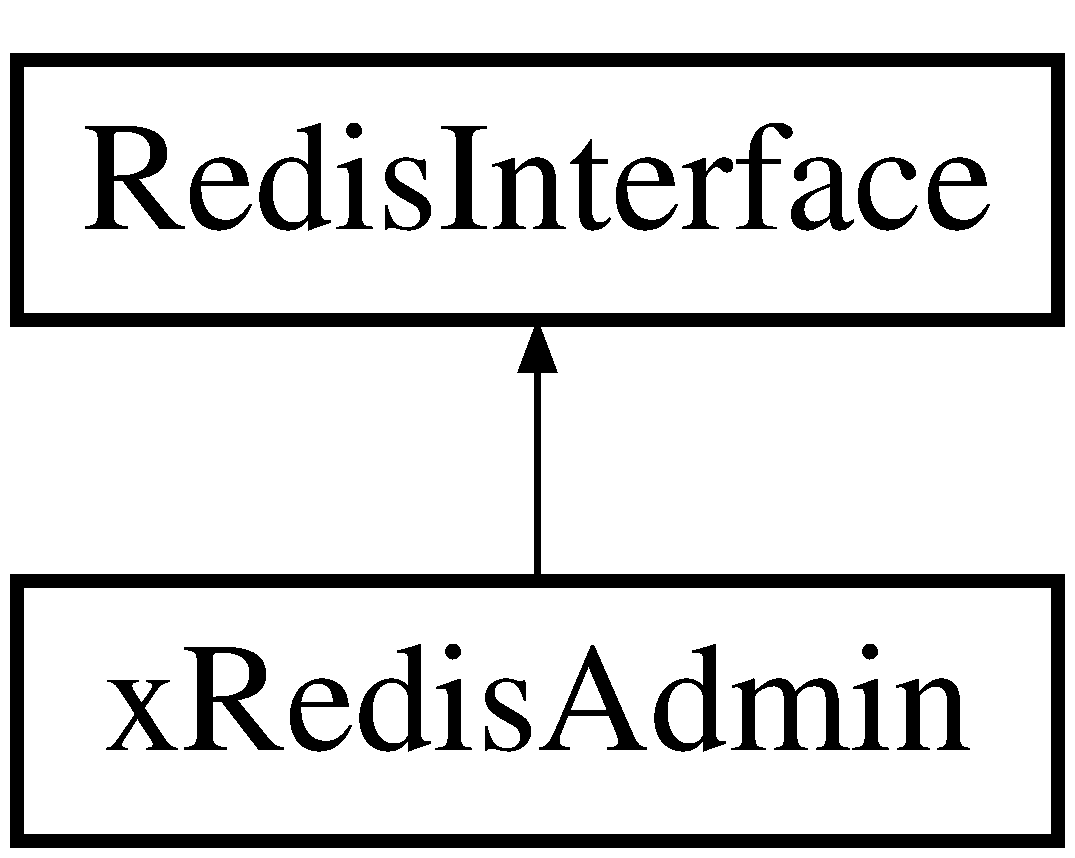
\includegraphics[height=2.000000cm]{classRedisInterface}
\end{center}
\end{figure}
\subsection*{Public Member Functions}
\begin{DoxyCompactItemize}
\item 
\hypertarget{classRedisInterface_afd325866fd98ca6e002b2702e5566ee5}{virtual std\-::string \hyperlink{classRedisInterface_afd325866fd98ca6e002b2702e5566ee5}{load} (const char $\ast$key)=0}\label{classRedisInterface_afd325866fd98ca6e002b2702e5566ee5}

\begin{DoxyCompactList}\small\item\em Load a value from Redis. \end{DoxyCompactList}\item 
\hypertarget{classRedisInterface_adb0d6e3f8a0848cbb6b346e57aeb3ad5}{virtual bool \hyperlink{classRedisInterface_adb0d6e3f8a0848cbb6b346e57aeb3ad5}{save} (const char $\ast$key, std\-::string msg)=0}\label{classRedisInterface_adb0d6e3f8a0848cbb6b346e57aeb3ad5}

\begin{DoxyCompactList}\small\item\em Save a value to Redis. \end{DoxyCompactList}\item 
\hypertarget{classRedisInterface_a3881f54b919852b7aaa231015775544e}{virtual bool \hyperlink{classRedisInterface_a3881f54b919852b7aaa231015775544e}{exists} (const char $\ast$key)=0}\label{classRedisInterface_a3881f54b919852b7aaa231015775544e}

\begin{DoxyCompactList}\small\item\em Does a key exist in Redis? \end{DoxyCompactList}\item 
\hypertarget{classRedisInterface_abb9b1fe2c11911648d62d431968fa04e}{virtual bool \hyperlink{classRedisInterface_abb9b1fe2c11911648d62d431968fa04e}{del} (const char $\ast$key)=0}\label{classRedisInterface_abb9b1fe2c11911648d62d431968fa04e}

\begin{DoxyCompactList}\small\item\em Delete a value from Redis. \end{DoxyCompactList}\item 
\hypertarget{classRedisInterface_ac327841b5c3d227be88f164495e32dd0}{virtual bool \hyperlink{classRedisInterface_ac327841b5c3d227be88f164495e32dd0}{expire} (const char $\ast$key, unsigned int second)=0}\label{classRedisInterface_ac327841b5c3d227be88f164495e32dd0}

\begin{DoxyCompactList}\small\item\em Expire a value in Redis after a specified number of seconds. \end{DoxyCompactList}\end{DoxyCompactItemize}


\subsection{Detailed Description}
The X\-Redis Admin. 

The X\-Redis Admin is responsible for all interactions with the Redis Key-\/\-Value Store. This is capable of connecting to single Redis instances or Clusters 

The documentation for this class was generated from the following file\-:\begin{DoxyCompactItemize}
\item 
lib/include/factory/redis\-\_\-interface.\-h\end{DoxyCompactItemize}

\hypertarget{classService}{\section{Service Class Reference}
\label{classService}\index{Service@{Service}}
}


A \hyperlink{classService}{Service} class which can be registered with Consul for each instance of a particular service.  




{\ttfamily \#include $<$service.\-h$>$}

Inheritance diagram for Service\-:\begin{figure}[H]
\begin{center}
\leavevmode
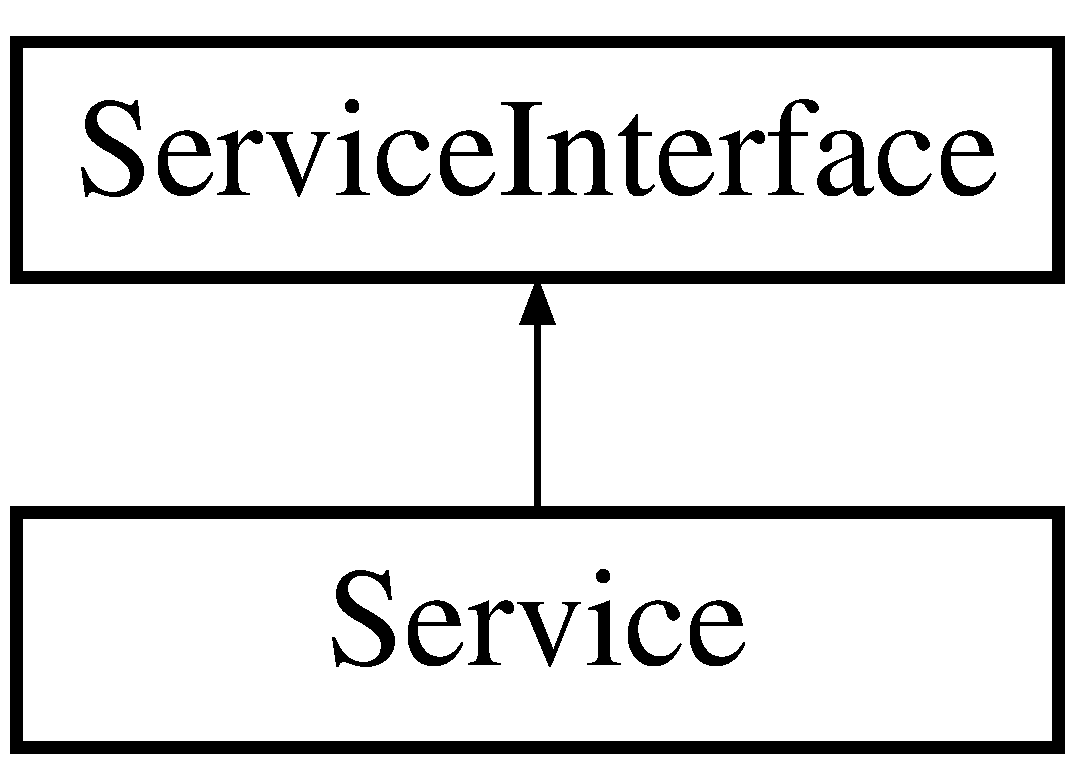
\includegraphics[height=2.000000cm]{classService}
\end{center}
\end{figure}
\subsection*{Public Member Functions}
\begin{DoxyCompactItemize}
\item 
\hypertarget{classService_acc246c9f7ed3c51e2d91d10fe257513f}{\hyperlink{classService_acc246c9f7ed3c51e2d91d10fe257513f}{Service} ()}\label{classService_acc246c9f7ed3c51e2d91d10fe257513f}

\begin{DoxyCompactList}\small\item\em Construct a \hyperlink{classService}{Service}. \end{DoxyCompactList}\item 
\hypertarget{classService_a5a2c138cda796995fd96f4d72961627e}{\hyperlink{classService_a5a2c138cda796995fd96f4d72961627e}{Service} (std\-::string new\-\_\-id, std\-::string new\-\_\-name)}\label{classService_a5a2c138cda796995fd96f4d72961627e}

\begin{DoxyCompactList}\small\item\em Construct a \hyperlink{classService}{Service}. \end{DoxyCompactList}\item 
\hypertarget{classService_a7fcbb48bac14e340ae490120dff8bc98}{\hyperlink{classService_a7fcbb48bac14e340ae490120dff8bc98}{Service} (std\-::string new\-\_\-id, std\-::string new\-\_\-name, std\-::string new\-\_\-address, std\-::string new\-\_\-port)}\label{classService_a7fcbb48bac14e340ae490120dff8bc98}

\begin{DoxyCompactList}\small\item\em Construct a \hyperlink{classService}{Service}. \end{DoxyCompactList}\item 
\hypertarget{classService_a3f17f6c4a5f8fd51034379e9dcae6d2c}{\hyperlink{classService_a3f17f6c4a5f8fd51034379e9dcae6d2c}{Service} (std\-::string new\-\_\-id, std\-::string new\-\_\-name, std\-::string new\-\_\-address, std\-::string new\-\_\-port, std\-::vector$<$ std\-::string $>$ new\-\_\-tags)}\label{classService_a3f17f6c4a5f8fd51034379e9dcae6d2c}

\begin{DoxyCompactList}\small\item\em Construct a \hyperlink{classService}{Service}. \end{DoxyCompactList}\item 
std\-::string \hyperlink{classService_a4a9e3ab8b1e7c82a7f624022906410f4}{to\-\_\-json} ()
\begin{DoxyCompactList}\small\item\em Convert the \hyperlink{classService}{Service} into a J\-S\-O\-N Message. \end{DoxyCompactList}\item 
\hypertarget{classService_adefcc615297a9cd243767f699468edb7}{std\-::string \hyperlink{classService_adefcc615297a9cd243767f699468edb7}{get\-\_\-id} ()}\label{classService_adefcc615297a9cd243767f699468edb7}

\begin{DoxyCompactList}\small\item\em Get the \hyperlink{classService}{Service} I\-D. \end{DoxyCompactList}\item 
\hypertarget{classService_a8b492e0a62e0457a8c5395fbcaa86c15}{std\-::string \hyperlink{classService_a8b492e0a62e0457a8c5395fbcaa86c15}{get\-\_\-name} ()}\label{classService_a8b492e0a62e0457a8c5395fbcaa86c15}

\begin{DoxyCompactList}\small\item\em Get the \hyperlink{classService}{Service} Name. \end{DoxyCompactList}\item 
\hypertarget{classService_acf3e71a82be6a4ba3915ad2039099da6}{std\-::string \hyperlink{classService_acf3e71a82be6a4ba3915ad2039099da6}{get\-\_\-address} ()}\label{classService_acf3e71a82be6a4ba3915ad2039099da6}

\begin{DoxyCompactList}\small\item\em Get the \hyperlink{classService}{Service} Address. \end{DoxyCompactList}\item 
\hypertarget{classService_acca3fc5199b3e85ce7a0cc875e515b72}{std\-::string \hyperlink{classService_acca3fc5199b3e85ce7a0cc875e515b72}{get\-\_\-port} ()}\label{classService_acca3fc5199b3e85ce7a0cc875e515b72}

\begin{DoxyCompactList}\small\item\em Get the \hyperlink{classService}{Service} Port. \end{DoxyCompactList}\item 
\hypertarget{classService_a2ea702a686d8561b43f6283647e18109}{void \hyperlink{classService_a2ea702a686d8561b43f6283647e18109}{set\-\_\-id} (std\-::string new\-\_\-id)}\label{classService_a2ea702a686d8561b43f6283647e18109}

\begin{DoxyCompactList}\small\item\em Set the \hyperlink{classService}{Service} I\-D. \end{DoxyCompactList}\item 
\hypertarget{classService_a8131d07e27a83148512ab82d70948dfc}{void \hyperlink{classService_a8131d07e27a83148512ab82d70948dfc}{set\-\_\-name} (std\-::string new\-\_\-name)}\label{classService_a8131d07e27a83148512ab82d70948dfc}

\begin{DoxyCompactList}\small\item\em Set the \hyperlink{classService}{Service} Name. \end{DoxyCompactList}\item 
\hypertarget{classService_a5f7aecf124823ad22e0c5265eb895cdc}{void \hyperlink{classService_a5f7aecf124823ad22e0c5265eb895cdc}{set\-\_\-address} (std\-::string new\-\_\-address)}\label{classService_a5f7aecf124823ad22e0c5265eb895cdc}

\begin{DoxyCompactList}\small\item\em Set the \hyperlink{classService}{Service} Address. \end{DoxyCompactList}\item 
\hypertarget{classService_a7bacad58f3bfb9f8d0bd757c89c0e4c4}{void \hyperlink{classService_a7bacad58f3bfb9f8d0bd757c89c0e4c4}{set\-\_\-port} (std\-::string new\-\_\-port)}\label{classService_a7bacad58f3bfb9f8d0bd757c89c0e4c4}

\begin{DoxyCompactList}\small\item\em Set the \hyperlink{classService}{Service} Port. \end{DoxyCompactList}\item 
\hypertarget{classService_ab3decdaff5d89934fe6b190c5bd74d57}{std\-::vector$<$ std\-::string $>$ {\bfseries get\-\_\-tags} ()}\label{classService_ab3decdaff5d89934fe6b190c5bd74d57}

\item 
\hypertarget{classService_ac700081515b84a002e4f9953c931727a}{void {\bfseries add\-\_\-tag} (std\-::string new\-\_\-tag)}\label{classService_ac700081515b84a002e4f9953c931727a}

\item 
\hypertarget{classService_a0bb490a55ed7bb2d82a760f980539bb0}{void {\bfseries clear\-\_\-tags} ()}\label{classService_a0bb490a55ed7bb2d82a760f980539bb0}

\item 
\hypertarget{classService_a7585975846335020ffe5b238bdb238f1}{int {\bfseries num\-\_\-tags} () const }\label{classService_a7585975846335020ffe5b238bdb238f1}

\item 
\hypertarget{classService_a5e8054b562abad283350834a5224f661}{\hyperlink{structHealthCheck}{Health\-Check} {\bfseries get\-\_\-check} ()}\label{classService_a5e8054b562abad283350834a5224f661}

\item 
\hypertarget{classService_a410b149173c0a01d4703f4f9312ff6ef}{void {\bfseries set\-\_\-check} (std\-::string scr, int interval\-\_\-seconds)}\label{classService_a410b149173c0a01d4703f4f9312ff6ef}

\end{DoxyCompactItemize}


\subsection{Detailed Description}
A \hyperlink{classService}{Service} class which can be registered with Consul for each instance of a particular service. 

An instance of this class can be instantiated by a service and is passed to the consul admin to register and de-\/register 

\subsection{Member Function Documentation}
\hypertarget{classService_a4a9e3ab8b1e7c82a7f624022906410f4}{\index{Service@{Service}!to\-\_\-json@{to\-\_\-json}}
\index{to\-\_\-json@{to\-\_\-json}!Service@{Service}}
\subsubsection[{to\-\_\-json}]{\setlength{\rightskip}{0pt plus 5cm}std\-::string Service\-::to\-\_\-json (
\begin{DoxyParamCaption}
{}
\end{DoxyParamCaption}
)\hspace{0.3cm}{\ttfamily [virtual]}}}\label{classService_a4a9e3ab8b1e7c82a7f624022906410f4}


Convert the \hyperlink{classService}{Service} into a J\-S\-O\-N Message. 

Method that allows the service to be transformed into a json message that can be sent via H\-T\-T\-P to a Consul instance 

Implements \hyperlink{classServiceInterface_a2c041d65d3e725f1cf8e2379f4620d58}{Service\-Interface}.



The documentation for this class was generated from the following file\-:\begin{DoxyCompactItemize}
\item 
lib/include/service.\-h\end{DoxyCompactItemize}

\hypertarget{classServiceComponentFactory}{\section{Service\-Component\-Factory Class Reference}
\label{classServiceComponentFactory}\index{Service\-Component\-Factory@{Service\-Component\-Factory}}
}


The Service Component Factory.  




{\ttfamily \#include $<$factory.\-h$>$}

\subsection*{Public Member Functions}
\begin{DoxyCompactItemize}
\item 
\hypertarget{classServiceComponentFactory_a0d91931c88bb8df41ee4f58b54c3cc8f}{\hyperlink{classServiceComponentFactory_a0d91931c88bb8df41ee4f58b54c3cc8f}{Service\-Component\-Factory} ()}\label{classServiceComponentFactory_a0d91931c88bb8df41ee4f58b54c3cc8f}

\begin{DoxyCompactList}\small\item\em Create a new Service Component Factory. \end{DoxyCompactList}\item 
\hypertarget{classServiceComponentFactory_a377472acb3040b7e06749ff48239ebd4}{\hyperlink{classServiceComponentFactory_a377472acb3040b7e06749ff48239ebd4}{$\sim$\-Service\-Component\-Factory} ()}\label{classServiceComponentFactory_a377472acb3040b7e06749ff48239ebd4}

\begin{DoxyCompactList}\small\item\em Delete a Service Component Factory. \end{DoxyCompactList}\item 
\hypertarget{classServiceComponentFactory_a7783b94ad65b0be4de8e4658f5b0ab4f}{\hyperlink{classCommandLineInterface}{Command\-Line\-Interface} $\ast$ \hyperlink{classServiceComponentFactory_a7783b94ad65b0be4de8e4658f5b0ab4f}{get\-\_\-command\-\_\-line\-\_\-interface} (int argc, char $\ast$argv\mbox{[}$\,$\mbox{]})}\label{classServiceComponentFactory_a7783b94ad65b0be4de8e4658f5b0ab4f}

\begin{DoxyCompactList}\small\item\em Get the Command Line Interface instance. \end{DoxyCompactList}\item 
\hypertarget{classServiceComponentFactory_a3c7d8ab1a2a2a88eac293d5a10610829}{\hyperlink{classuuidInterface}{uuid\-Interface} $\ast$ \hyperlink{classServiceComponentFactory_a3c7d8ab1a2a2a88eac293d5a10610829}{get\-\_\-uuid\-\_\-interface} ()}\label{classServiceComponentFactory_a3c7d8ab1a2a2a88eac293d5a10610829}

\begin{DoxyCompactList}\small\item\em Get the U\-U\-I\-D Interface instance. \end{DoxyCompactList}\item 
\hypertarget{classServiceComponentFactory_a231204b51354b045ea3d5fff7b07ec94}{\hyperlink{classHttpInterface}{Http\-Interface} $\ast$ \hyperlink{classServiceComponentFactory_a231204b51354b045ea3d5fff7b07ec94}{get\-\_\-http\-\_\-interface} ()}\label{classServiceComponentFactory_a231204b51354b045ea3d5fff7b07ec94}

\begin{DoxyCompactList}\small\item\em Get the H\-T\-T\-P Interface instance. \end{DoxyCompactList}\item 
\hypertarget{classServiceComponentFactory_a8f1a67c4158e2e9fc844563b7c35dc15}{\hyperlink{classConsulInterface}{Consul\-Interface} $\ast$ \hyperlink{classServiceComponentFactory_a8f1a67c4158e2e9fc844563b7c35dc15}{get\-\_\-consul\-\_\-interface} (std\-::string caddr)}\label{classServiceComponentFactory_a8f1a67c4158e2e9fc844563b7c35dc15}

\begin{DoxyCompactList}\small\item\em Get a Consul Interface instance. \end{DoxyCompactList}\item 
\hypertarget{classServiceComponentFactory_a18fc7b189a89281312ae594db57bf9f3}{\hyperlink{classServiceInterface}{Service\-Interface} $\ast$ \hyperlink{classServiceComponentFactory_a18fc7b189a89281312ae594db57bf9f3}{get\-\_\-service\-\_\-interface} ()}\label{classServiceComponentFactory_a18fc7b189a89281312ae594db57bf9f3}

\begin{DoxyCompactList}\small\item\em Get a Service Interface instance. \end{DoxyCompactList}\item 
\hypertarget{classServiceComponentFactory_ae0f4ffe321b3ef4f0677a319a29bb7ac}{\hyperlink{classServiceInterface}{Service\-Interface} $\ast$ \hyperlink{classServiceComponentFactory_ae0f4ffe321b3ef4f0677a319a29bb7ac}{get\-\_\-service\-\_\-interface} (std\-::string new\-\_\-id, std\-::string new\-\_\-name)}\label{classServiceComponentFactory_ae0f4ffe321b3ef4f0677a319a29bb7ac}

\begin{DoxyCompactList}\small\item\em Get a Service Interface instance. \end{DoxyCompactList}\item 
\hypertarget{classServiceComponentFactory_a00f71ee92a14c3d850d8dd7e808d4b19}{\hyperlink{classServiceInterface}{Service\-Interface} $\ast$ \hyperlink{classServiceComponentFactory_a00f71ee92a14c3d850d8dd7e808d4b19}{get\-\_\-service\-\_\-interface} (std\-::string new\-\_\-id, std\-::string new\-\_\-name, std\-::string new\-\_\-address, std\-::string new\-\_\-port)}\label{classServiceComponentFactory_a00f71ee92a14c3d850d8dd7e808d4b19}

\begin{DoxyCompactList}\small\item\em Get a Service Interface instance. \end{DoxyCompactList}\item 
\hypertarget{classServiceComponentFactory_a3461ba8dac008cf74b117b626a1851b2}{\hyperlink{classServiceInterface}{Service\-Interface} $\ast$ \hyperlink{classServiceComponentFactory_a3461ba8dac008cf74b117b626a1851b2}{get\-\_\-service\-\_\-interface} (std\-::string new\-\_\-id, std\-::string new\-\_\-name, std\-::string new\-\_\-address, std\-::string new\-\_\-port, std\-::vector$<$ std\-::string $>$ new\-\_\-tags)}\label{classServiceComponentFactory_a3461ba8dac008cf74b117b626a1851b2}

\begin{DoxyCompactList}\small\item\em Get a Service Interface instance. \end{DoxyCompactList}\item 
\hypertarget{classServiceComponentFactory_ab0054b867f4ceb06217a035a8909ca65}{\hyperlink{classCouchbaseInterface}{Couchbase\-Interface} $\ast$ \hyperlink{classServiceComponentFactory_ab0054b867f4ceb06217a035a8909ca65}{get\-\_\-couchbase\-\_\-interface} (const char $\ast$conn)}\label{classServiceComponentFactory_ab0054b867f4ceb06217a035a8909ca65}

\begin{DoxyCompactList}\small\item\em Get a Couchbase Interface instance. \end{DoxyCompactList}\item 
\hypertarget{classServiceComponentFactory_ae0c38d94599bcf148704d3436a529d13}{\hyperlink{classCouchbaseInterface}{Couchbase\-Interface} $\ast$ \hyperlink{classServiceComponentFactory_ae0c38d94599bcf148704d3436a529d13}{get\-\_\-couchbase\-\_\-interface} (const char $\ast$conn, const char $\ast$pswd)}\label{classServiceComponentFactory_ae0c38d94599bcf148704d3436a529d13}

\begin{DoxyCompactList}\small\item\em Get a Couchbase Interface instance for a password protected D\-B. \end{DoxyCompactList}\item 
\hypertarget{classServiceComponentFactory_a960660c5cb312c1cdb6b20bd87c2e2d5}{\hyperlink{classRedisInterface}{Redis\-Interface} $\ast$ \hyperlink{classServiceComponentFactory_a960660c5cb312c1cdb6b20bd87c2e2d5}{get\-\_\-redis\-\_\-cluster\-\_\-interface} (std\-::vector$<$ \hyperlink{structRedisConnChain}{Redis\-Conn\-Chain} $>$ Redis\-Connection\-List)}\label{classServiceComponentFactory_a960660c5cb312c1cdb6b20bd87c2e2d5}

\begin{DoxyCompactList}\small\item\em Get a Redis Cluster Interface instance. \end{DoxyCompactList}\item 
\hypertarget{classServiceComponentFactory_aa0bd65f6cb0e588ab97d51ba15733d31}{\hyperlink{classLoggingInterface}{Logging\-Interface} $\ast$ \hyperlink{classServiceComponentFactory_aa0bd65f6cb0e588ab97d51ba15733d31}{get\-\_\-logging\-\_\-interface} (std\-::string init\-File\-Name)}\label{classServiceComponentFactory_aa0bd65f6cb0e588ab97d51ba15733d31}

\begin{DoxyCompactList}\small\item\em Get a Logging Interface instance. \end{DoxyCompactList}\item 
\hypertarget{classServiceComponentFactory_a1d20e28c7b7c88d458598278245ae499}{\hyperlink{classZmqio}{Zmqio} $\ast$ \hyperlink{classServiceComponentFactory_a1d20e28c7b7c88d458598278245ae499}{get\-\_\-zmq\-\_\-outbound\-\_\-interface} (std\-::string conn\-\_\-str)}\label{classServiceComponentFactory_a1d20e28c7b7c88d458598278245ae499}

\begin{DoxyCompactList}\small\item\em Get a Z\-M\-Q Outbound Interface instance. \end{DoxyCompactList}\item 
\hypertarget{classServiceComponentFactory_a01ba58fc37d73d758774635d723dc7f9}{\hyperlink{classZmqio}{Zmqio} $\ast$ \hyperlink{classServiceComponentFactory_a01ba58fc37d73d758774635d723dc7f9}{get\-\_\-zmq\-\_\-inbound\-\_\-interface} (std\-::string conn\-\_\-str)}\label{classServiceComponentFactory_a01ba58fc37d73d758774635d723dc7f9}

\begin{DoxyCompactList}\small\item\em Get a Z\-M\-Q Inbound Interface instance. \end{DoxyCompactList}\end{DoxyCompactItemize}


\subsection{Detailed Description}
The Service Component Factory. 

The Service Component Factory tracks the various objects exposed by the framework and passes back instances of interfaces. This allows for the publicly exposed methods to be independent of the implementations. 

The documentation for this class was generated from the following file\-:\begin{DoxyCompactItemize}
\item 
lib/include/factory.\-h\end{DoxyCompactItemize}

\hypertarget{classServiceInterface}{}\section{Service\+Interface Class Reference}
\label{classServiceInterface}\index{Service\+Interface@{Service\+Interface}}


A Service class which can be registered with Consul for each instance of a particular service.  




{\ttfamily \#include $<$consul\+\_\+interface.\+h$>$}

\subsection*{Public Member Functions}
\begin{DoxyCompactItemize}
\item 
virtual std\+::string \hyperlink{classServiceInterface_a2c041d65d3e725f1cf8e2379f4620d58}{to\+\_\+json} ()=0
\begin{DoxyCompactList}\small\item\em Convert the Service into a J\+S\+ON Message. \end{DoxyCompactList}\item 
virtual std\+::string \hyperlink{classServiceInterface_a0ba731e4d379cbeddc852304b470c617}{get\+\_\+id} ()=0\hypertarget{classServiceInterface_a0ba731e4d379cbeddc852304b470c617}{}\label{classServiceInterface_a0ba731e4d379cbeddc852304b470c617}

\begin{DoxyCompactList}\small\item\em Get the Service ID. \end{DoxyCompactList}\item 
virtual std\+::string \hyperlink{classServiceInterface_aed2140959e23f98cd0cca1a101646384}{get\+\_\+name} ()=0\hypertarget{classServiceInterface_aed2140959e23f98cd0cca1a101646384}{}\label{classServiceInterface_aed2140959e23f98cd0cca1a101646384}

\begin{DoxyCompactList}\small\item\em Get the Service Name. \end{DoxyCompactList}\item 
virtual std\+::string \hyperlink{classServiceInterface_a6c4fd6eff9e1c8eed5dfed301d2f8047}{get\+\_\+address} ()=0\hypertarget{classServiceInterface_a6c4fd6eff9e1c8eed5dfed301d2f8047}{}\label{classServiceInterface_a6c4fd6eff9e1c8eed5dfed301d2f8047}

\begin{DoxyCompactList}\small\item\em Get the Service Address. \end{DoxyCompactList}\item 
virtual std\+::string \hyperlink{classServiceInterface_a7c8a328711f7fb019a9f7dadcb897cb0}{get\+\_\+port} ()=0\hypertarget{classServiceInterface_a7c8a328711f7fb019a9f7dadcb897cb0}{}\label{classServiceInterface_a7c8a328711f7fb019a9f7dadcb897cb0}

\begin{DoxyCompactList}\small\item\em Get the Service Port. \end{DoxyCompactList}\item 
virtual void \hyperlink{classServiceInterface_aade793bb679fa00cd34194a3623c554a}{set\+\_\+id} (std\+::string new\+\_\+id)=0\hypertarget{classServiceInterface_aade793bb679fa00cd34194a3623c554a}{}\label{classServiceInterface_aade793bb679fa00cd34194a3623c554a}

\begin{DoxyCompactList}\small\item\em Set the Service ID. \end{DoxyCompactList}\item 
virtual void \hyperlink{classServiceInterface_ac9b2d1a785b665ef3c575f5877148511}{set\+\_\+name} (std\+::string new\+\_\+name)=0\hypertarget{classServiceInterface_ac9b2d1a785b665ef3c575f5877148511}{}\label{classServiceInterface_ac9b2d1a785b665ef3c575f5877148511}

\begin{DoxyCompactList}\small\item\em Set the Service Name. \end{DoxyCompactList}\item 
virtual void \hyperlink{classServiceInterface_a619fb75631f816d547d2ad3efeae2bf5}{set\+\_\+address} (std\+::string new\+\_\+address)=0\hypertarget{classServiceInterface_a619fb75631f816d547d2ad3efeae2bf5}{}\label{classServiceInterface_a619fb75631f816d547d2ad3efeae2bf5}

\begin{DoxyCompactList}\small\item\em Set the Service Address. \end{DoxyCompactList}\item 
virtual void \hyperlink{classServiceInterface_a2c9385fbc567949560dc7972e6a7059e}{set\+\_\+port} (std\+::string new\+\_\+port)=0\hypertarget{classServiceInterface_a2c9385fbc567949560dc7972e6a7059e}{}\label{classServiceInterface_a2c9385fbc567949560dc7972e6a7059e}

\begin{DoxyCompactList}\small\item\em Set the Service Port. \end{DoxyCompactList}\item 
virtual std\+::vector$<$ std\+::string $>$ \hyperlink{classServiceInterface_afdc1ce12ef5ff09cf82e3d0f8ea7724a}{get\+\_\+tags} ()=0\hypertarget{classServiceInterface_afdc1ce12ef5ff09cf82e3d0f8ea7724a}{}\label{classServiceInterface_afdc1ce12ef5ff09cf82e3d0f8ea7724a}

\begin{DoxyCompactList}\small\item\em Get the tags. \end{DoxyCompactList}\item 
virtual void \hyperlink{classServiceInterface_ac8b80c9301fa04ea295acecd88b9cc42}{add\+\_\+tag} (std\+::string new\+\_\+tag)=0\hypertarget{classServiceInterface_ac8b80c9301fa04ea295acecd88b9cc42}{}\label{classServiceInterface_ac8b80c9301fa04ea295acecd88b9cc42}

\begin{DoxyCompactList}\small\item\em Add a tag. \end{DoxyCompactList}\item 
virtual void \hyperlink{classServiceInterface_a3e27c216421be0e92984b07a095f1279}{clear\+\_\+tags} ()=0\hypertarget{classServiceInterface_a3e27c216421be0e92984b07a095f1279}{}\label{classServiceInterface_a3e27c216421be0e92984b07a095f1279}

\begin{DoxyCompactList}\small\item\em Clear the tags. \end{DoxyCompactList}\item 
virtual int \hyperlink{classServiceInterface_aad0434e39242a47048659a1243fab46e}{num\+\_\+tags} () const =0\hypertarget{classServiceInterface_aad0434e39242a47048659a1243fab46e}{}\label{classServiceInterface_aad0434e39242a47048659a1243fab46e}

\begin{DoxyCompactList}\small\item\em How many tags are there? \end{DoxyCompactList}\item 
virtual \hyperlink{structHealthCheck}{Health\+Check} \hyperlink{classServiceInterface_afa5e0a43120dcd89dfcf7ae8aa086217}{get\+\_\+check} ()=0\hypertarget{classServiceInterface_afa5e0a43120dcd89dfcf7ae8aa086217}{}\label{classServiceInterface_afa5e0a43120dcd89dfcf7ae8aa086217}

\begin{DoxyCompactList}\small\item\em Get the health checks. \end{DoxyCompactList}\item 
virtual void \hyperlink{classServiceInterface_a32065df2094fa5a53708f5ff3944195b}{set\+\_\+check} (std\+::string scr, int interval\+\_\+seconds)=0\hypertarget{classServiceInterface_a32065df2094fa5a53708f5ff3944195b}{}\label{classServiceInterface_a32065df2094fa5a53708f5ff3944195b}

\begin{DoxyCompactList}\small\item\em Add a check. \end{DoxyCompactList}\end{DoxyCompactItemize}


\subsection{Detailed Description}
A Service class which can be registered with Consul for each instance of a particular service. 

An instance of this class can be instantiated by a service and is passed to the consul admin to register and de-\/register 

\subsection{Member Function Documentation}
\index{Service\+Interface@{Service\+Interface}!to\+\_\+json@{to\+\_\+json}}
\index{to\+\_\+json@{to\+\_\+json}!Service\+Interface@{Service\+Interface}}
\subsubsection[{\texorpdfstring{to\+\_\+json()=0}{to_json()=0}}]{\setlength{\rightskip}{0pt plus 5cm}virtual std\+::string Service\+Interface\+::to\+\_\+json (
\begin{DoxyParamCaption}
{}
\end{DoxyParamCaption}
)\hspace{0.3cm}{\ttfamily [pure virtual]}}\hypertarget{classServiceInterface_a2c041d65d3e725f1cf8e2379f4620d58}{}\label{classServiceInterface_a2c041d65d3e725f1cf8e2379f4620d58}


Convert the Service into a J\+S\+ON Message. 

Method that allows the service to be transformed into a json message that can be sent via H\+T\+TP to a Consul instance 

The documentation for this class was generated from the following file\+:\begin{DoxyCompactItemize}
\item 
aossl/consul/include/consul\+\_\+interface.\+h\end{DoxyCompactItemize}

\hypertarget{classuuidAdmin}{\section{uuid\-Admin Class Reference}
\label{classuuidAdmin}\index{uuid\-Admin@{uuid\-Admin}}
}


U\-U\-I\-D Admin.  




{\ttfamily \#include $<$uuid\-\_\-admin.\-h$>$}

Inheritance diagram for uuid\-Admin\-:\begin{figure}[H]
\begin{center}
\leavevmode
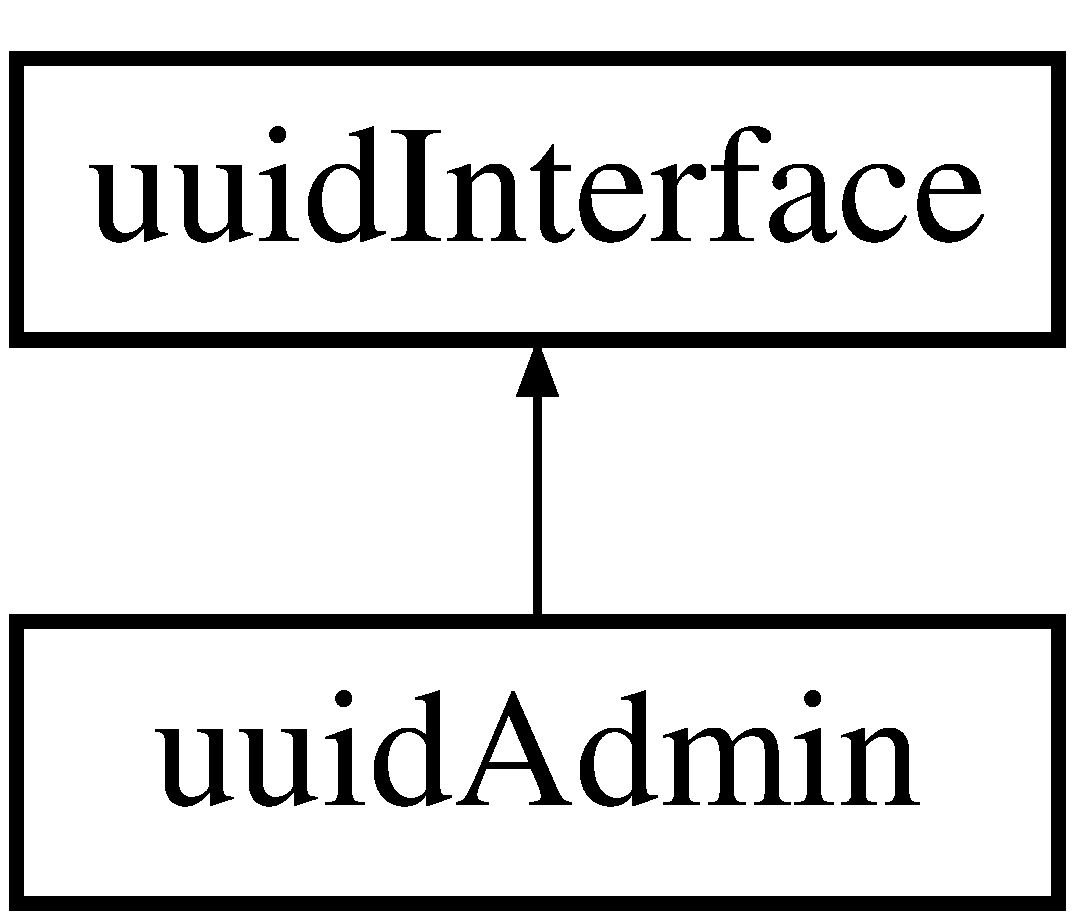
\includegraphics[height=2.000000cm]{classuuidAdmin}
\end{center}
\end{figure}
\subsection*{Public Member Functions}
\begin{DoxyCompactItemize}
\item 
std\-::string \hyperlink{classuuidAdmin_a344f39f4c1e15cf72e64b3544312d7ed}{generate} ()
\begin{DoxyCompactList}\small\item\em Generate a new U\-U\-I\-D. \end{DoxyCompactList}\end{DoxyCompactItemize}


\subsection{Detailed Description}
U\-U\-I\-D Admin. 

The U\-U\-I\-D Admin is in charge of generating any Universally Unique I\-D's that are required throughout program execution 

\subsection{Member Function Documentation}
\hypertarget{classuuidAdmin_a344f39f4c1e15cf72e64b3544312d7ed}{\index{uuid\-Admin@{uuid\-Admin}!generate@{generate}}
\index{generate@{generate}!uuidAdmin@{uuid\-Admin}}
\subsubsection[{generate}]{\setlength{\rightskip}{0pt plus 5cm}std\-::string uuid\-Admin\-::generate (
\begin{DoxyParamCaption}
{}
\end{DoxyParamCaption}
)\hspace{0.3cm}{\ttfamily [virtual]}}}\label{classuuidAdmin_a344f39f4c1e15cf72e64b3544312d7ed}


Generate a new U\-U\-I\-D. 

The method will generate on the means of generation present on your system In some cases, this may result in U\-U\-I\-D's being generated that pose a security risk. In this case, that fact will be clearly called out in the logs, and it is recommended that production systems are tested to ensure that U\-U\-I\-D's are generated in a safe manner 

Implements \hyperlink{classuuidInterface_ae1696692de5b139246154c8d32d44797}{uuid\-Interface}.



The documentation for this class was generated from the following file\-:\begin{DoxyCompactItemize}
\item 
lib/include/uuid\-\_\-admin.\-h\end{DoxyCompactItemize}

\hypertarget{classuuidInterface}{\section{uuid\-Interface Class Reference}
\label{classuuidInterface}\index{uuid\-Interface@{uuid\-Interface}}
}


U\-U\-I\-D Admin.  




{\ttfamily \#include $<$uuid\-\_\-interface.\-h$>$}

Inheritance diagram for uuid\-Interface\-:\begin{figure}[H]
\begin{center}
\leavevmode
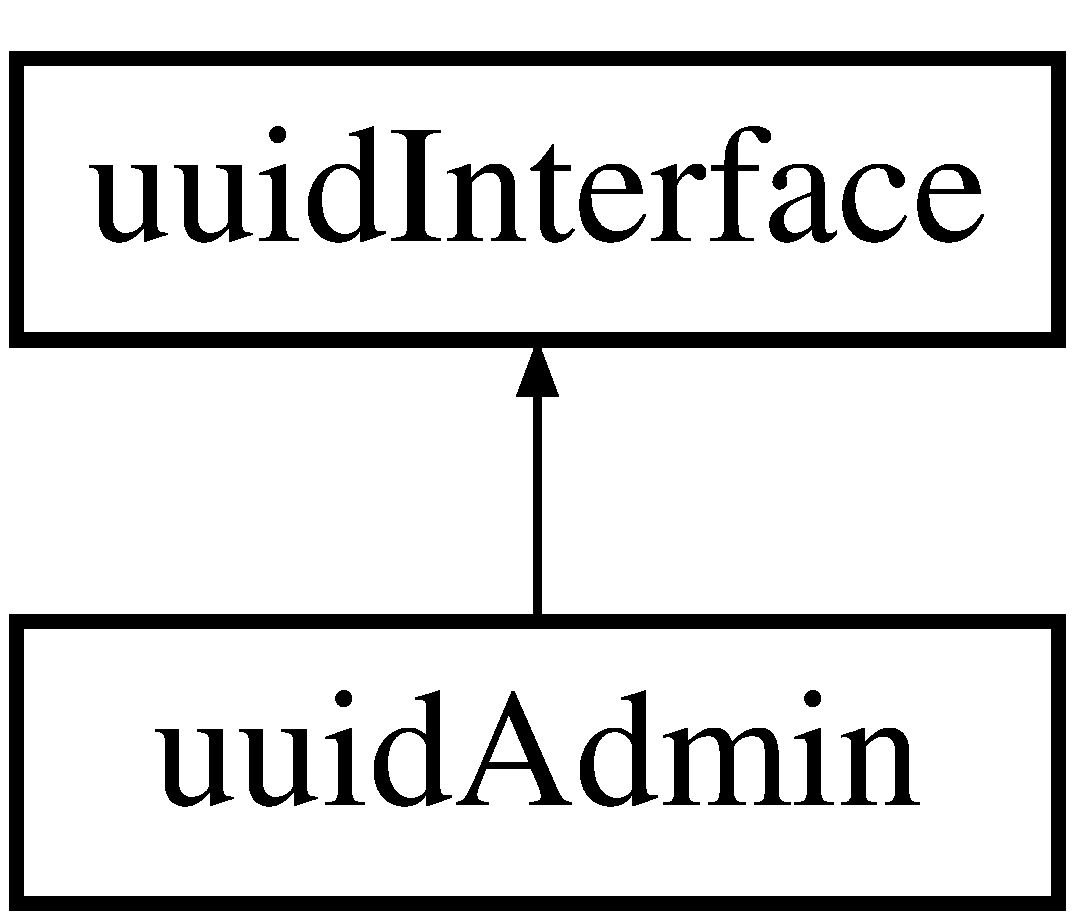
\includegraphics[height=2.000000cm]{classuuidInterface}
\end{center}
\end{figure}
\subsection*{Public Member Functions}
\begin{DoxyCompactItemize}
\item 
virtual std\-::string \hyperlink{classuuidInterface_ae1696692de5b139246154c8d32d44797}{generate} ()=0
\begin{DoxyCompactList}\small\item\em Generate a new U\-U\-I\-D. \end{DoxyCompactList}\end{DoxyCompactItemize}


\subsection{Detailed Description}
U\-U\-I\-D Admin. 

The U\-U\-I\-D Admin is in charge of generating any Universally Unique I\-D's that are required throughout program execution 

\subsection{Member Function Documentation}
\hypertarget{classuuidInterface_ae1696692de5b139246154c8d32d44797}{\index{uuid\-Interface@{uuid\-Interface}!generate@{generate}}
\index{generate@{generate}!uuidInterface@{uuid\-Interface}}
\subsubsection[{generate}]{\setlength{\rightskip}{0pt plus 5cm}virtual std\-::string uuid\-Interface\-::generate (
\begin{DoxyParamCaption}
{}
\end{DoxyParamCaption}
)\hspace{0.3cm}{\ttfamily [pure virtual]}}}\label{classuuidInterface_ae1696692de5b139246154c8d32d44797}


Generate a new U\-U\-I\-D. 

The method will generate on the means of generation present on your system In some cases, this may result in U\-U\-I\-D's being generated that pose a security risk. In this case, that fact will be clearly called out in the logs, and it is recommended that production systems are tested to ensure that U\-U\-I\-D's are generated in a safe manner 

Implemented in \hyperlink{classuuidAdmin_a344f39f4c1e15cf72e64b3544312d7ed}{uuid\-Admin}.



The documentation for this class was generated from the following file\-:\begin{DoxyCompactItemize}
\item 
lib/include/factory/uuid\-\_\-interface.\-h\end{DoxyCompactItemize}

\hypertarget{classWriteable}{\section{Writeable Class Reference}
\label{classWriteable}\index{Writeable@{Writeable}}
}


The \hyperlink{classWriteable}{Writeable} Interface.  




{\ttfamily \#include $<$writeable.\-h$>$}

\subsection*{Public Member Functions}
\begin{DoxyCompactItemize}
\item 
\hypertarget{classWriteable_ac546538ca16d6448efa54701d4ff8e73}{virtual std\-::string \hyperlink{classWriteable_ac546538ca16d6448efa54701d4ff8e73}{get\-\_\-key} ()=0}\label{classWriteable_ac546538ca16d6448efa54701d4ff8e73}

\begin{DoxyCompactList}\small\item\em Get the Object Key. \end{DoxyCompactList}\item 
\hypertarget{classWriteable_a9332d6b96c8930605ebab49faee06c2f}{virtual bool \hyperlink{classWriteable_a9332d6b96c8930605ebab49faee06c2f}{set\-\_\-key} (std\-::string new\-\_\-key)=0}\label{classWriteable_a9332d6b96c8930605ebab49faee06c2f}

\begin{DoxyCompactList}\small\item\em Set the Object Key. \end{DoxyCompactList}\item 
\hypertarget{classWriteable_a3439d4a6364404cea695b393da1b6d93}{virtual std\-::string \hyperlink{classWriteable_a3439d4a6364404cea695b393da1b6d93}{to\-\_\-json} ()=0}\label{classWriteable_a3439d4a6364404cea695b393da1b6d93}

\begin{DoxyCompactList}\small\item\em Convert the object to J\-S\-O\-N. \end{DoxyCompactList}\end{DoxyCompactItemize}


\subsection{Detailed Description}
The \hyperlink{classWriteable}{Writeable} Interface. 

The \hyperlink{classWriteable}{Writeable} interface is used by the D\-B Administrators In order to define a class of objects that can be written to a J\-S\-O\-N Document, and therefore sent to a Document-\/based Database 

The documentation for this class was generated from the following file\-:\begin{DoxyCompactItemize}
\item 
lib/include/factory/writeable.\-h\end{DoxyCompactItemize}

\hypertarget{classxRedisAdmin}{\section{x\-Redis\-Admin Class Reference}
\label{classxRedisAdmin}\index{x\-Redis\-Admin@{x\-Redis\-Admin}}
}


The X\-Redis Admin.  




{\ttfamily \#include $<$xredis\-\_\-admin.\-h$>$}

\subsection*{Public Member Functions}
\begin{DoxyCompactItemize}
\item 
\hypertarget{classxRedisAdmin_ae59b7611ff2d0cd4549794e4622d1251}{\hyperlink{classxRedisAdmin_ae59b7611ff2d0cd4549794e4622d1251}{x\-Redis\-Admin} (Redis\-Node conn\-\_\-list\mbox{[}$\,$\mbox{]}, int conn\-\_\-list\-\_\-size)}\label{classxRedisAdmin_ae59b7611ff2d0cd4549794e4622d1251}

\begin{DoxyCompactList}\small\item\em Construct a new X\-Redis Admin with a given list of Redis Connections. \end{DoxyCompactList}\item 
\hypertarget{classxRedisAdmin_a06d156c9ba252cbd5bd48d1f199a7e97}{\hyperlink{classxRedisAdmin_a06d156c9ba252cbd5bd48d1f199a7e97}{$\sim$x\-Redis\-Admin} ()}\label{classxRedisAdmin_a06d156c9ba252cbd5bd48d1f199a7e97}

\begin{DoxyCompactList}\small\item\em Delete the X\-Redis Admin. \end{DoxyCompactList}\item 
\hypertarget{classxRedisAdmin_aa19abdf1562f23acd7193756bfbf1c2a}{std\-::string \hyperlink{classxRedisAdmin_aa19abdf1562f23acd7193756bfbf1c2a}{load} (const char $\ast$key)}\label{classxRedisAdmin_aa19abdf1562f23acd7193756bfbf1c2a}

\begin{DoxyCompactList}\small\item\em Load a value from Redis. \end{DoxyCompactList}\item 
\hypertarget{classxRedisAdmin_ab5a36717fae762eeb88213a7fb349c14}{bool \hyperlink{classxRedisAdmin_ab5a36717fae762eeb88213a7fb349c14}{save} (const char $\ast$key, std\-::string msg)}\label{classxRedisAdmin_ab5a36717fae762eeb88213a7fb349c14}

\begin{DoxyCompactList}\small\item\em Save a value to Redis. \end{DoxyCompactList}\item 
\hypertarget{classxRedisAdmin_afe27654a8ff1783b03f5dc403d2c82e6}{bool \hyperlink{classxRedisAdmin_afe27654a8ff1783b03f5dc403d2c82e6}{exists} (const char $\ast$key)}\label{classxRedisAdmin_afe27654a8ff1783b03f5dc403d2c82e6}

\begin{DoxyCompactList}\small\item\em Does a key exist in Redis? \end{DoxyCompactList}\item 
\hypertarget{classxRedisAdmin_aec6bb15ec6d7764423e6abddac9a7c3c}{bool \hyperlink{classxRedisAdmin_aec6bb15ec6d7764423e6abddac9a7c3c}{del} (const char $\ast$key)}\label{classxRedisAdmin_aec6bb15ec6d7764423e6abddac9a7c3c}

\begin{DoxyCompactList}\small\item\em Delete a value from Redis. \end{DoxyCompactList}\item 
\hypertarget{classxRedisAdmin_a97cac4467038a8b4309029ed13563ff2}{bool \hyperlink{classxRedisAdmin_a97cac4467038a8b4309029ed13563ff2}{expire} (const char $\ast$key, unsigned int second)}\label{classxRedisAdmin_a97cac4467038a8b4309029ed13563ff2}

\begin{DoxyCompactList}\small\item\em Expire a value in Redis after a specified number of seconds. \end{DoxyCompactList}\end{DoxyCompactItemize}


\subsection{Detailed Description}
The X\-Redis Admin. 

The X\-Redis Admin is responsible for all interactions with the Redis Key-\/\-Value Store. This is capable of connecting to single Redis instances or Clusters 

The documentation for this class was generated from the following files\-:\begin{DoxyCompactItemize}
\item 
lib/include/xredis\-\_\-admin.\-h\item 
lib/xredis\-\_\-admin.\-cpp\end{DoxyCompactItemize}

\hypertarget{classZmqi}{\section{Zmqi Class Reference}
\label{classZmqi}\index{Zmqi@{Zmqi}}
}


An Inbound Z\-M\-Q Manager.  




{\ttfamily \#include $<$zmqio.\-h$>$}

Inheritance diagram for Zmqi\-:\begin{figure}[H]
\begin{center}
\leavevmode
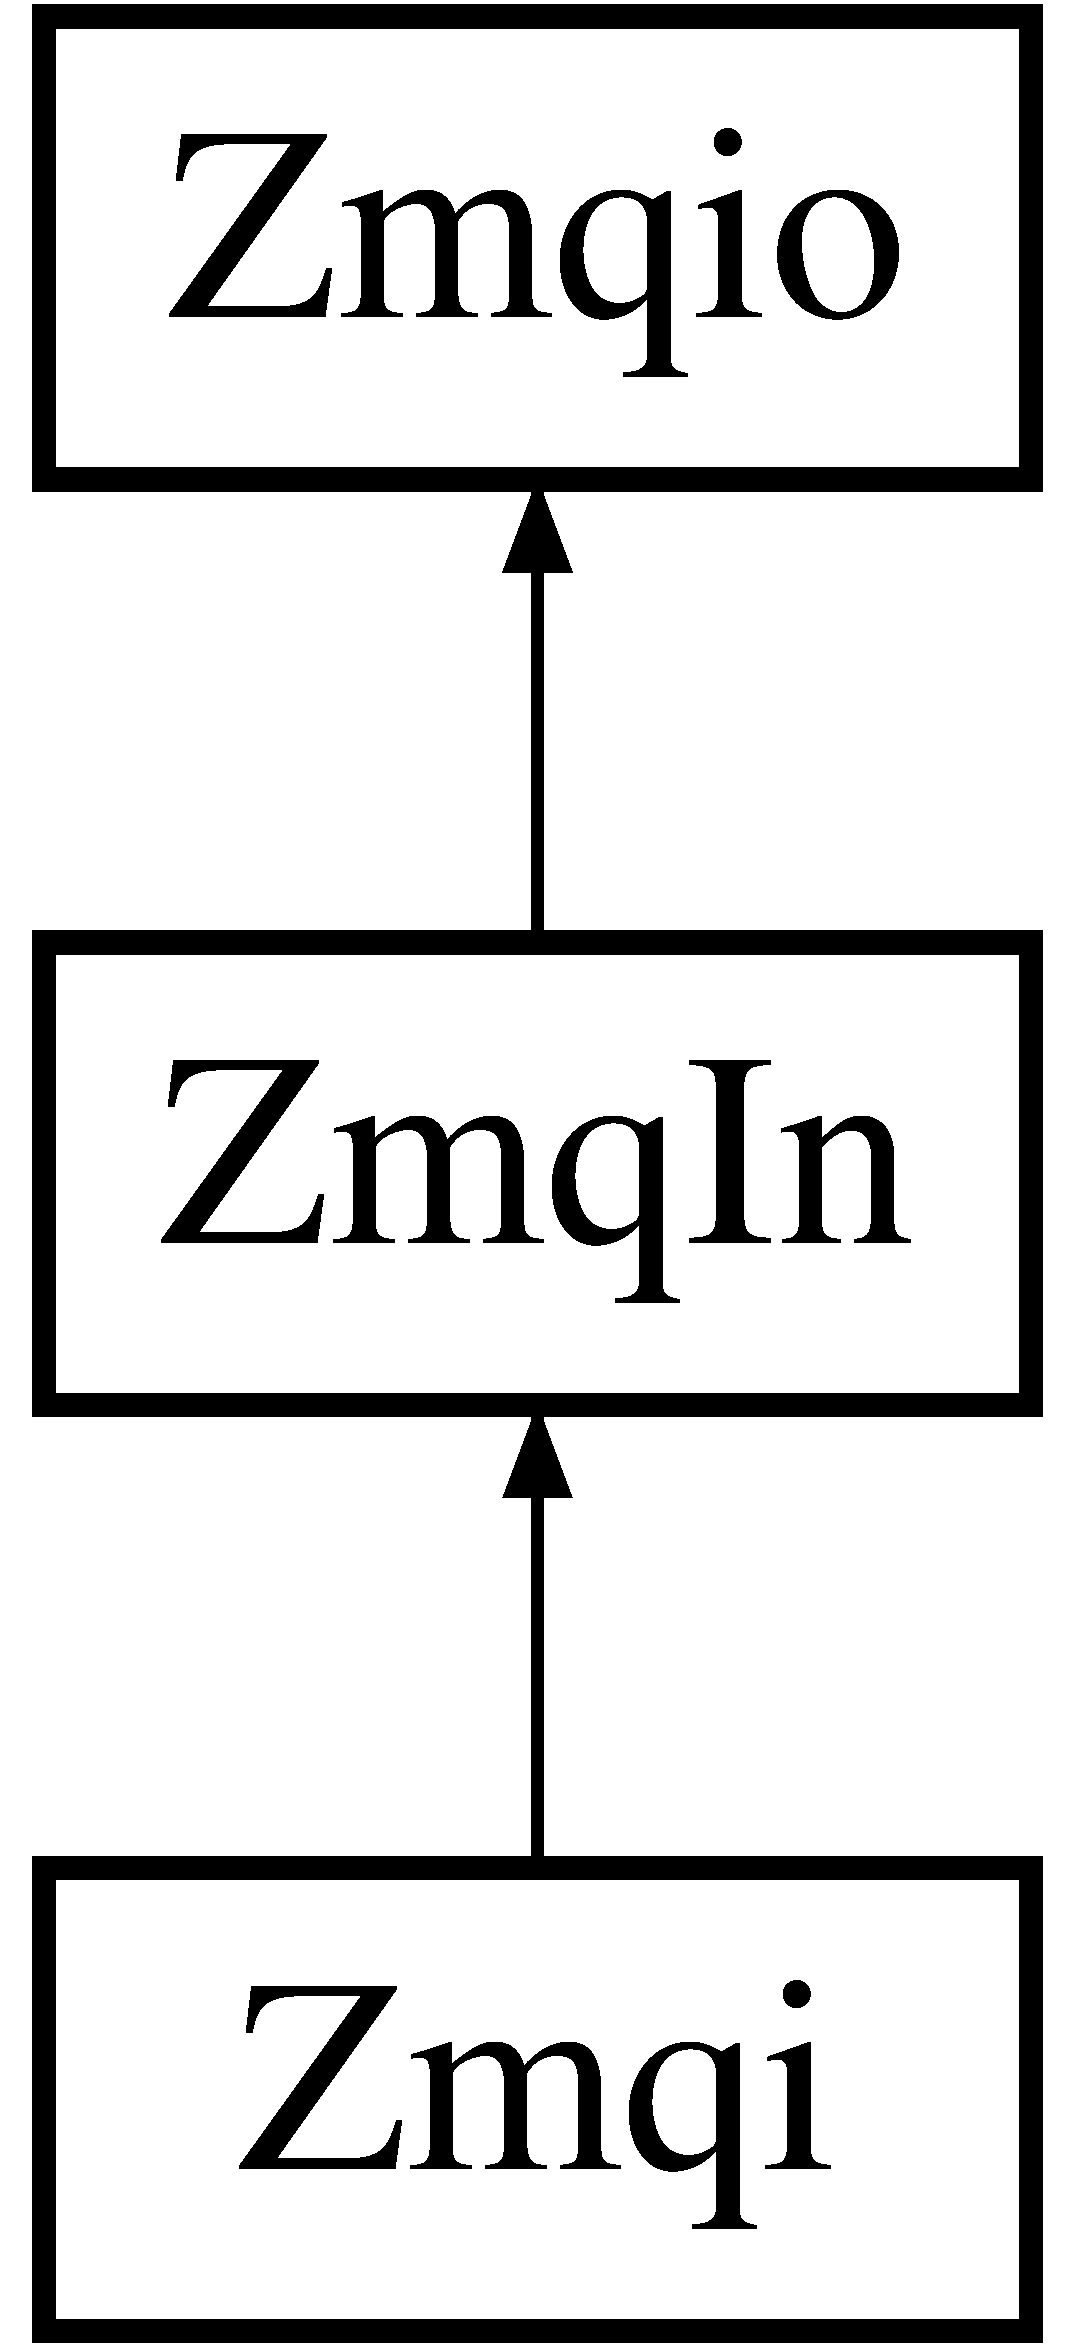
\includegraphics[height=2.000000cm]{classZmqi}
\end{center}
\end{figure}
\subsection*{Public Member Functions}
\begin{DoxyCompactItemize}
\item 
\hypertarget{classZmqi_aa83e723dca3ad4734a5482019a156a4e}{\hyperlink{classZmqi_aa83e723dca3ad4734a5482019a156a4e}{Zmqi} (zmq\-::context\-\_\-t \&context)}\label{classZmqi_aa83e723dca3ad4734a5482019a156a4e}

\begin{DoxyCompactList}\small\item\em Build a new Inbound Z\-M\-Q Manager. \end{DoxyCompactList}\item 
\hypertarget{classZmqi_aa90b541fb0bc12f79d65e04f4a58b9fb}{\hyperlink{classZmqi_aa90b541fb0bc12f79d65e04f4a58b9fb}{$\sim$\-Zmqi} ()}\label{classZmqi_aa90b541fb0bc12f79d65e04f4a58b9fb}

\begin{DoxyCompactList}\small\item\em Destroy the Z\-M\-Q\-I Manager. \end{DoxyCompactList}\item 
\hypertarget{classZmqi_ad54a77411f2149c346298512966b13cb}{void \hyperlink{classZmqi_ad54a77411f2149c346298512966b13cb}{bind} (std\-::string conn\-\_\-str)}\label{classZmqi_ad54a77411f2149c346298512966b13cb}

\begin{DoxyCompactList}\small\item\em Bind on the given conn\-\_\-str. \end{DoxyCompactList}\item 
\hypertarget{classZmqi_acdc3a5addbd2236f0dc25d120edf05af}{std\-::string \hyperlink{classZmqi_acdc3a5addbd2236f0dc25d120edf05af}{recv} ()}\label{classZmqi_acdc3a5addbd2236f0dc25d120edf05af}

\begin{DoxyCompactList}\small\item\em Recieve a message on the port. \end{DoxyCompactList}\item 
\hypertarget{classZmqi_a6543637f6b8dd0c01ef0aa773a40fdce}{void \hyperlink{classZmqi_a6543637f6b8dd0c01ef0aa773a40fdce}{send} (const char $\ast$msg, int msg\-\_\-size)}\label{classZmqi_a6543637f6b8dd0c01ef0aa773a40fdce}

\begin{DoxyCompactList}\small\item\em Send a message on the port. \end{DoxyCompactList}\item 
\hypertarget{classZmqi_a3bf1017f5893fb138c0c776e6b8e050f}{void \hyperlink{classZmqi_a3bf1017f5893fb138c0c776e6b8e050f}{send} (std\-::string msg)}\label{classZmqi_a3bf1017f5893fb138c0c776e6b8e050f}

\begin{DoxyCompactList}\small\item\em Send a string on the port. \end{DoxyCompactList}\end{DoxyCompactItemize}


\subsection{Detailed Description}
An Inbound Z\-M\-Q Manager. 

Acts as the Responder (Server) in the Z\-M\-Q Sockets Recieve, then Send 

The documentation for this class was generated from the following files\-:\begin{DoxyCompactItemize}
\item 
lib/include/zmqio.\-h\item 
lib/zmqio.\-cpp\end{DoxyCompactItemize}

\hypertarget{classZmqIn}{\section{Zmq\-In Class Reference}
\label{classZmqIn}\index{Zmq\-In@{Zmq\-In}}
}


An Inbound Z\-M\-Q Manager.  




{\ttfamily \#include $<$zmq\-\_\-interface.\-h$>$}

Inheritance diagram for Zmq\-In\-:\begin{figure}[H]
\begin{center}
\leavevmode
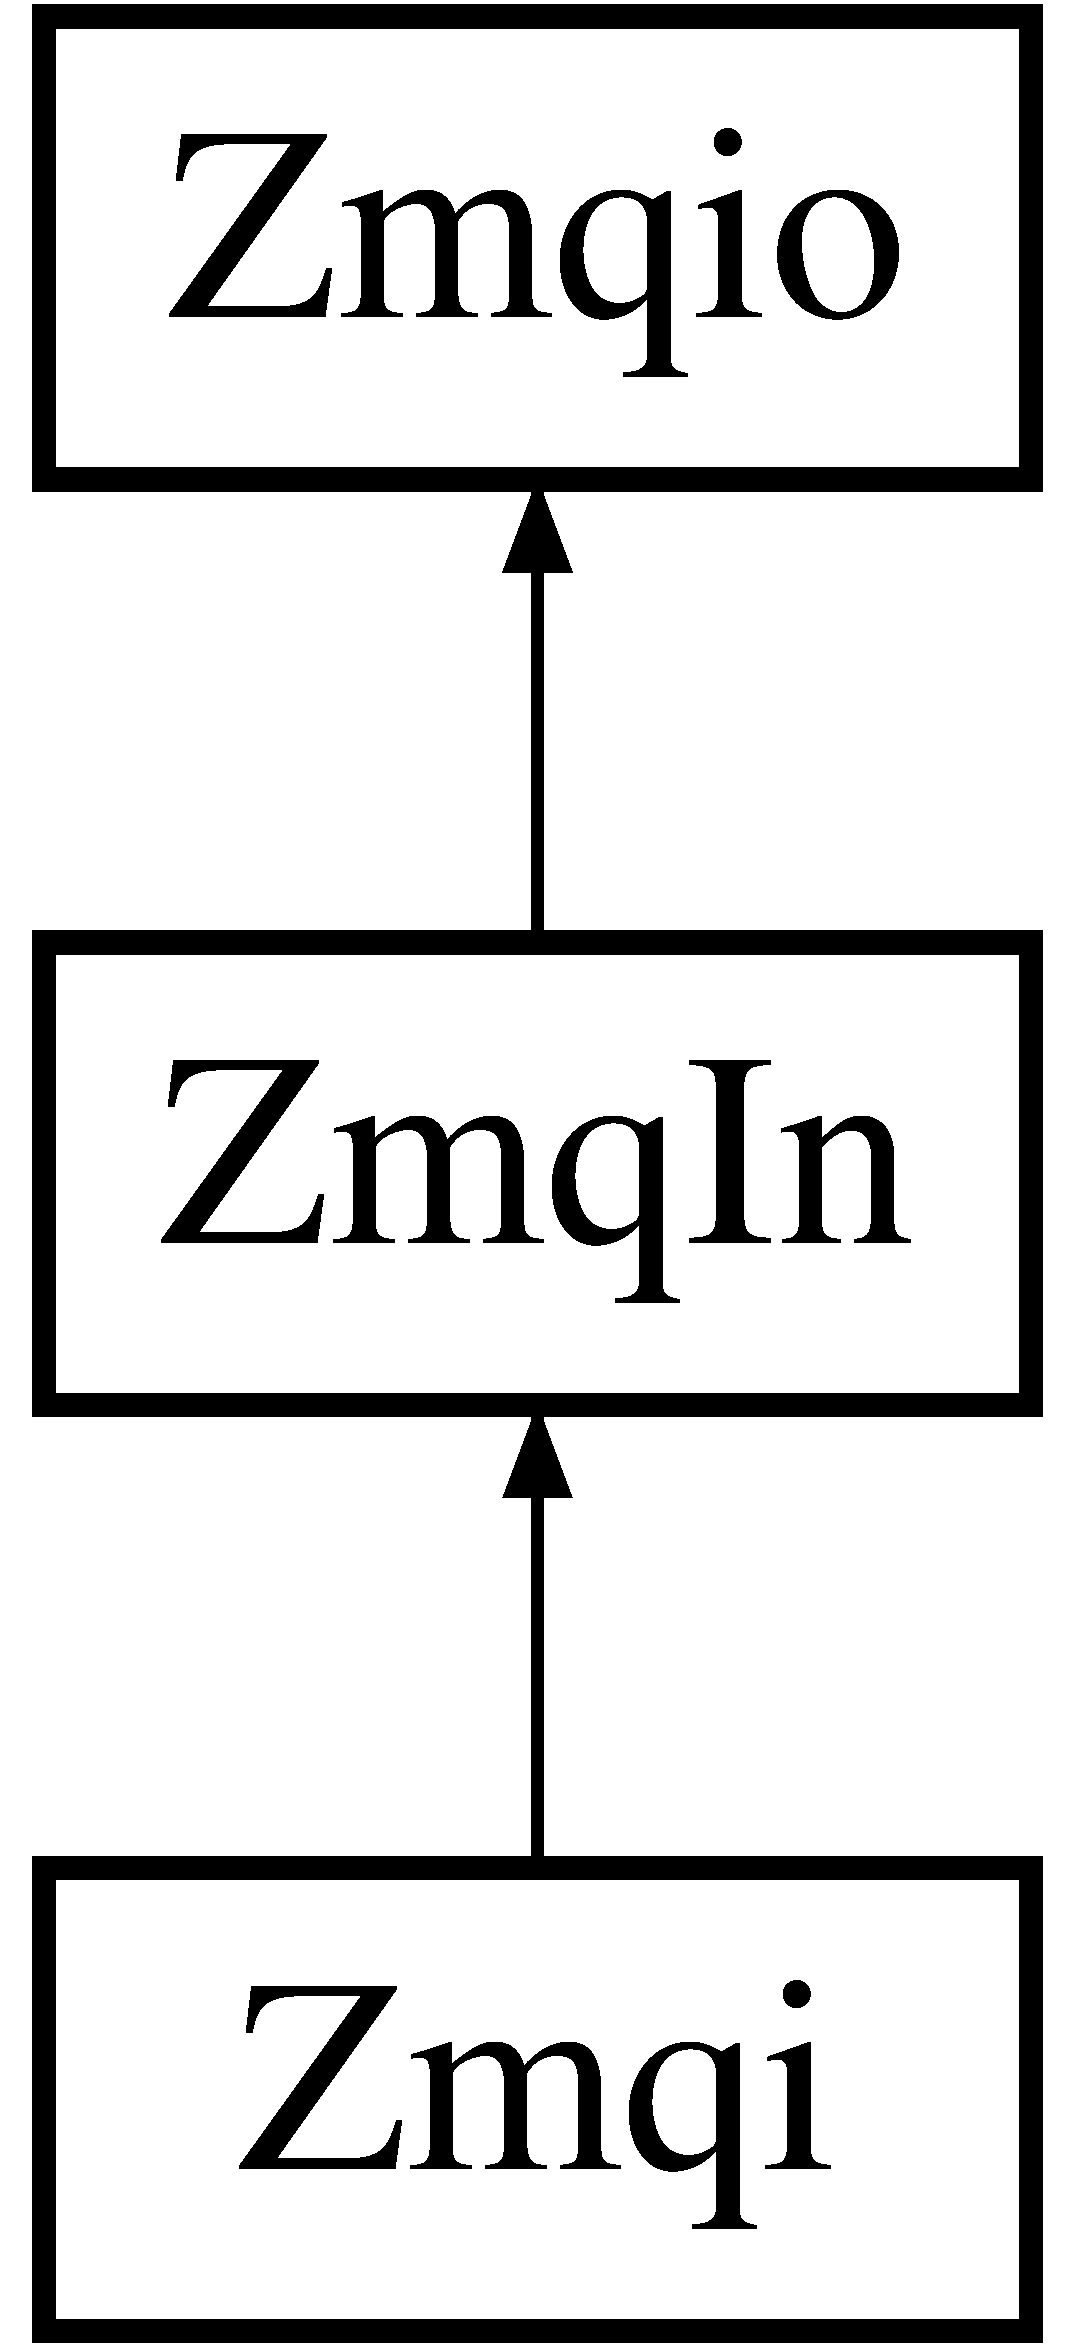
\includegraphics[height=2.000000cm]{classZmqIn}
\end{center}
\end{figure}
\subsection*{Public Member Functions}
\begin{DoxyCompactItemize}
\item 
\hypertarget{classZmqIn_ad6037a187635f7d46bab5da961156751}{virtual void \hyperlink{classZmqIn_ad6037a187635f7d46bab5da961156751}{bind} (std\-::string conn\-\_\-str)=0}\label{classZmqIn_ad6037a187635f7d46bab5da961156751}

\begin{DoxyCompactList}\small\item\em Bind on the given conn\-\_\-str. \end{DoxyCompactList}\item 
\hypertarget{classZmqIn_a375de593defd4c2cf3adebad063950fe}{virtual std\-::string \hyperlink{classZmqIn_a375de593defd4c2cf3adebad063950fe}{recv} ()=0}\label{classZmqIn_a375de593defd4c2cf3adebad063950fe}

\begin{DoxyCompactList}\small\item\em Recieve a message on the port. \end{DoxyCompactList}\item 
\hypertarget{classZmqIn_ad2a35cc76a5b0b2412fda5418f708e60}{virtual void \hyperlink{classZmqIn_ad2a35cc76a5b0b2412fda5418f708e60}{send} (const char $\ast$msg, int msg\-\_\-size)=0}\label{classZmqIn_ad2a35cc76a5b0b2412fda5418f708e60}

\begin{DoxyCompactList}\small\item\em Send a message on the port. \end{DoxyCompactList}\item 
\hypertarget{classZmqIn_adf4165c263ddc5b68099b93b9f37f592}{virtual void \hyperlink{classZmqIn_adf4165c263ddc5b68099b93b9f37f592}{send} (std\-::string msg)=0}\label{classZmqIn_adf4165c263ddc5b68099b93b9f37f592}

\begin{DoxyCompactList}\small\item\em Send a string on the port. \end{DoxyCompactList}\item 
\hypertarget{classZmqIn_a1b7ed3f43e1796a5a0cdd090f69ae932}{virtual void \hyperlink{classZmqIn_a1b7ed3f43e1796a5a0cdd090f69ae932}{subscribe} (std\-::string filter)=0}\label{classZmqIn_a1b7ed3f43e1796a5a0cdd090f69ae932}

\begin{DoxyCompactList}\small\item\em Subscribe on a particular filter (only effective for Pub/\-Sub) \end{DoxyCompactList}\end{DoxyCompactItemize}


\subsection{Detailed Description}
An Inbound Z\-M\-Q Manager. 

Acts as the Responder (Server) in the Z\-M\-Q Sockets Recieve, then Send 

The documentation for this class was generated from the following file\-:\begin{DoxyCompactItemize}
\item 
lib/include/factory/zmq\-\_\-interface.\-h\end{DoxyCompactItemize}

\hypertarget{classZmqio}{\section{Zmqio Class Reference}
\label{classZmqio}\index{Zmqio@{Zmqio}}
}


An Interface for Z\-M\-Q\-I\-O.  




{\ttfamily \#include $<$zmq\-\_\-interface.\-h$>$}

Inheritance diagram for Zmqio\-:\begin{figure}[H]
\begin{center}
\leavevmode
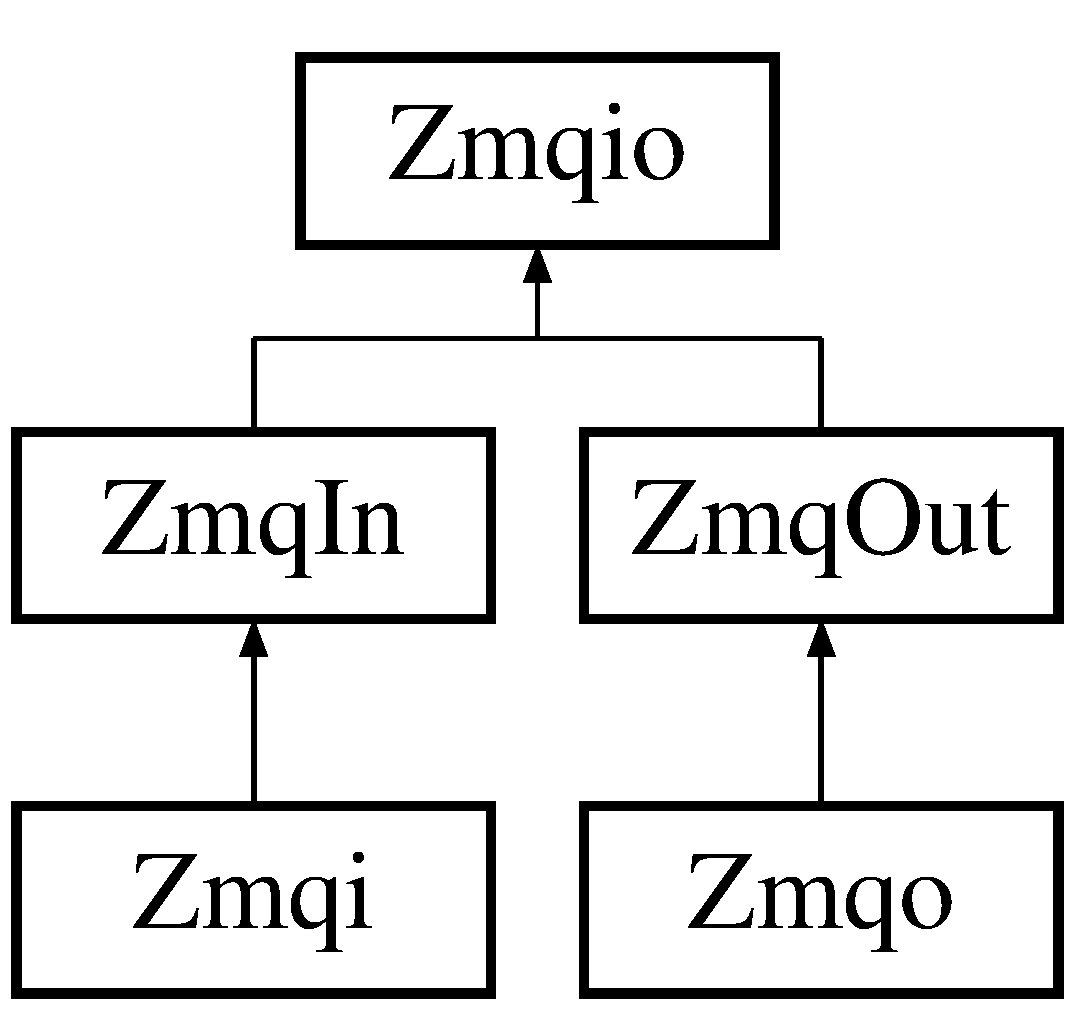
\includegraphics[height=2.000000cm]{classZmqio}
\end{center}
\end{figure}
\subsection*{Public Member Functions}
\begin{DoxyCompactItemize}
\item 
\hypertarget{classZmqio_a9365ac0ed42905898502e16857997acc}{virtual std\-::string \hyperlink{classZmqio_a9365ac0ed42905898502e16857997acc}{recv} ()=0}\label{classZmqio_a9365ac0ed42905898502e16857997acc}

\begin{DoxyCompactList}\small\item\em Recieve a message on the port. \end{DoxyCompactList}\item 
\hypertarget{classZmqio_a858e00e8ac5c4d1d60c665fa7c0716f0}{virtual void \hyperlink{classZmqio_a858e00e8ac5c4d1d60c665fa7c0716f0}{send} (const char $\ast$msg, int msg\-\_\-size)=0}\label{classZmqio_a858e00e8ac5c4d1d60c665fa7c0716f0}

\begin{DoxyCompactList}\small\item\em Send a message on the port. \end{DoxyCompactList}\item 
\hypertarget{classZmqio_a079f5752b553ddb2e5a2da565bcf162c}{virtual void \hyperlink{classZmqio_a079f5752b553ddb2e5a2da565bcf162c}{send} (std\-::string msg)=0}\label{classZmqio_a079f5752b553ddb2e5a2da565bcf162c}

\begin{DoxyCompactList}\small\item\em Send a string on the port. \end{DoxyCompactList}\item 
\hypertarget{classZmqio_aa315934401c5a3ba2eb502c16a3a6aca}{virtual void \hyperlink{classZmqio_aa315934401c5a3ba2eb502c16a3a6aca}{subscribe} (std\-::string filter)=0}\label{classZmqio_aa315934401c5a3ba2eb502c16a3a6aca}

\begin{DoxyCompactList}\small\item\em Subscribe on a particular filter (only effective for Pub/\-Sub) \end{DoxyCompactList}\end{DoxyCompactItemize}


\subsection{Detailed Description}
An Interface for Z\-M\-Q\-I\-O. 

Defines the methods that the Z\-M\-Q Managers must implement send \& recv, as well as subscribe 

The documentation for this class was generated from the following file\-:\begin{DoxyCompactItemize}
\item 
lib/include/factory/zmq\-\_\-interface.\-h\end{DoxyCompactItemize}

\hypertarget{classZmqo}{\section{Zmqo Class Reference}
\label{classZmqo}\index{Zmqo@{Zmqo}}
}


An Outbound Z\-M\-Q Manager.  




{\ttfamily \#include $<$zmqio.\-h$>$}

Inheritance diagram for Zmqo\-:\begin{figure}[H]
\begin{center}
\leavevmode
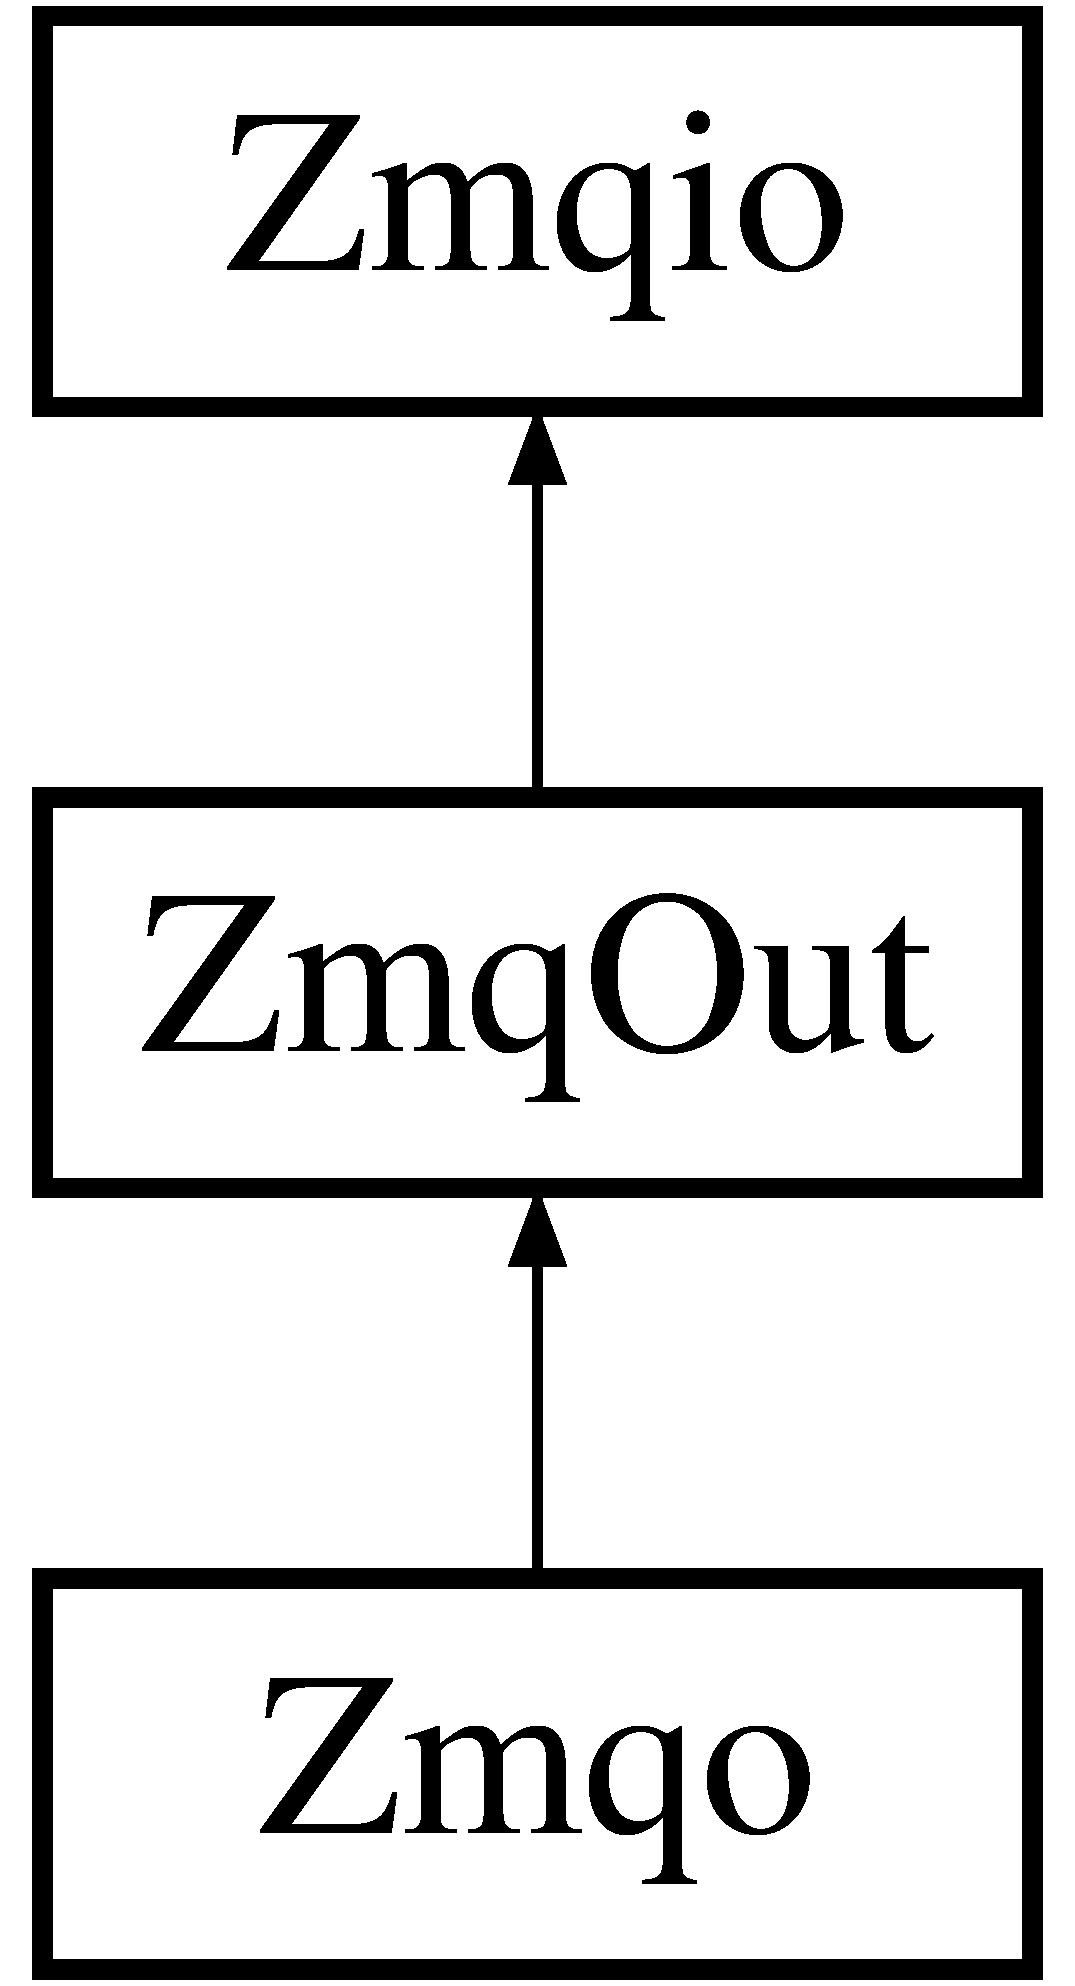
\includegraphics[height=2.000000cm]{classZmqo}
\end{center}
\end{figure}
\subsection*{Public Member Functions}
\begin{DoxyCompactItemize}
\item 
\hypertarget{classZmqo_a1572f05607e0ec993e3409dbce857f4f}{\hyperlink{classZmqo_a1572f05607e0ec993e3409dbce857f4f}{Zmqo} (zmq\-::context\-\_\-t \&context)}\label{classZmqo_a1572f05607e0ec993e3409dbce857f4f}

\begin{DoxyCompactList}\small\item\em Build a new Outbound Z\-M\-Q Manager. \end{DoxyCompactList}\item 
\hypertarget{classZmqo_a72472d8a881f468c06da8c0f23e80494}{\hyperlink{classZmqo_a72472d8a881f468c06da8c0f23e80494}{$\sim$\-Zmqo} ()}\label{classZmqo_a72472d8a881f468c06da8c0f23e80494}

\begin{DoxyCompactList}\small\item\em Destroy the Z\-M\-Q\-O Manager. \end{DoxyCompactList}\item 
\hypertarget{classZmqo_aa81909a34c542dd66d0079400ad3f3e9}{void \hyperlink{classZmqo_aa81909a34c542dd66d0079400ad3f3e9}{connect} (std\-::string conn\-\_\-str)}\label{classZmqo_aa81909a34c542dd66d0079400ad3f3e9}

\begin{DoxyCompactList}\small\item\em Connect to the given conn\-\_\-str. \end{DoxyCompactList}\item 
\hypertarget{classZmqo_a8142cd31df8cc0d75a617dc9ae84ff37}{void \hyperlink{classZmqo_a8142cd31df8cc0d75a617dc9ae84ff37}{send} (const char $\ast$msg, int msg\-\_\-size)}\label{classZmqo_a8142cd31df8cc0d75a617dc9ae84ff37}

\begin{DoxyCompactList}\small\item\em Send a message on the port. \end{DoxyCompactList}\item 
\hypertarget{classZmqo_ae5184a9dfc2017f3c9d62bd51c457f53}{void \hyperlink{classZmqo_ae5184a9dfc2017f3c9d62bd51c457f53}{send} (std\-::string msg)}\label{classZmqo_ae5184a9dfc2017f3c9d62bd51c457f53}

\begin{DoxyCompactList}\small\item\em Send a string on the port. \end{DoxyCompactList}\item 
\hypertarget{classZmqo_afdf8372877361a581595ccb4983f8110}{std\-::string \hyperlink{classZmqo_afdf8372877361a581595ccb4983f8110}{recv} ()}\label{classZmqo_afdf8372877361a581595ccb4983f8110}

\begin{DoxyCompactList}\small\item\em Recieve a message on the port. \end{DoxyCompactList}\end{DoxyCompactItemize}


\subsection{Detailed Description}
An Outbound Z\-M\-Q Manager. 

Acts as the Requestor (Client) in the Z\-M\-Q Sockets Send, then Recieve 

The documentation for this class was generated from the following files\-:\begin{DoxyCompactItemize}
\item 
lib/include/zmqio.\-h\item 
lib/zmqio.\-cpp\end{DoxyCompactItemize}

\hypertarget{classZmqOut}{\section{Zmq\-Out Class Reference}
\label{classZmqOut}\index{Zmq\-Out@{Zmq\-Out}}
}


An Outbound Z\-M\-Q Manager.  




{\ttfamily \#include $<$zmq\-\_\-interface.\-h$>$}

Inheritance diagram for Zmq\-Out\-:\begin{figure}[H]
\begin{center}
\leavevmode
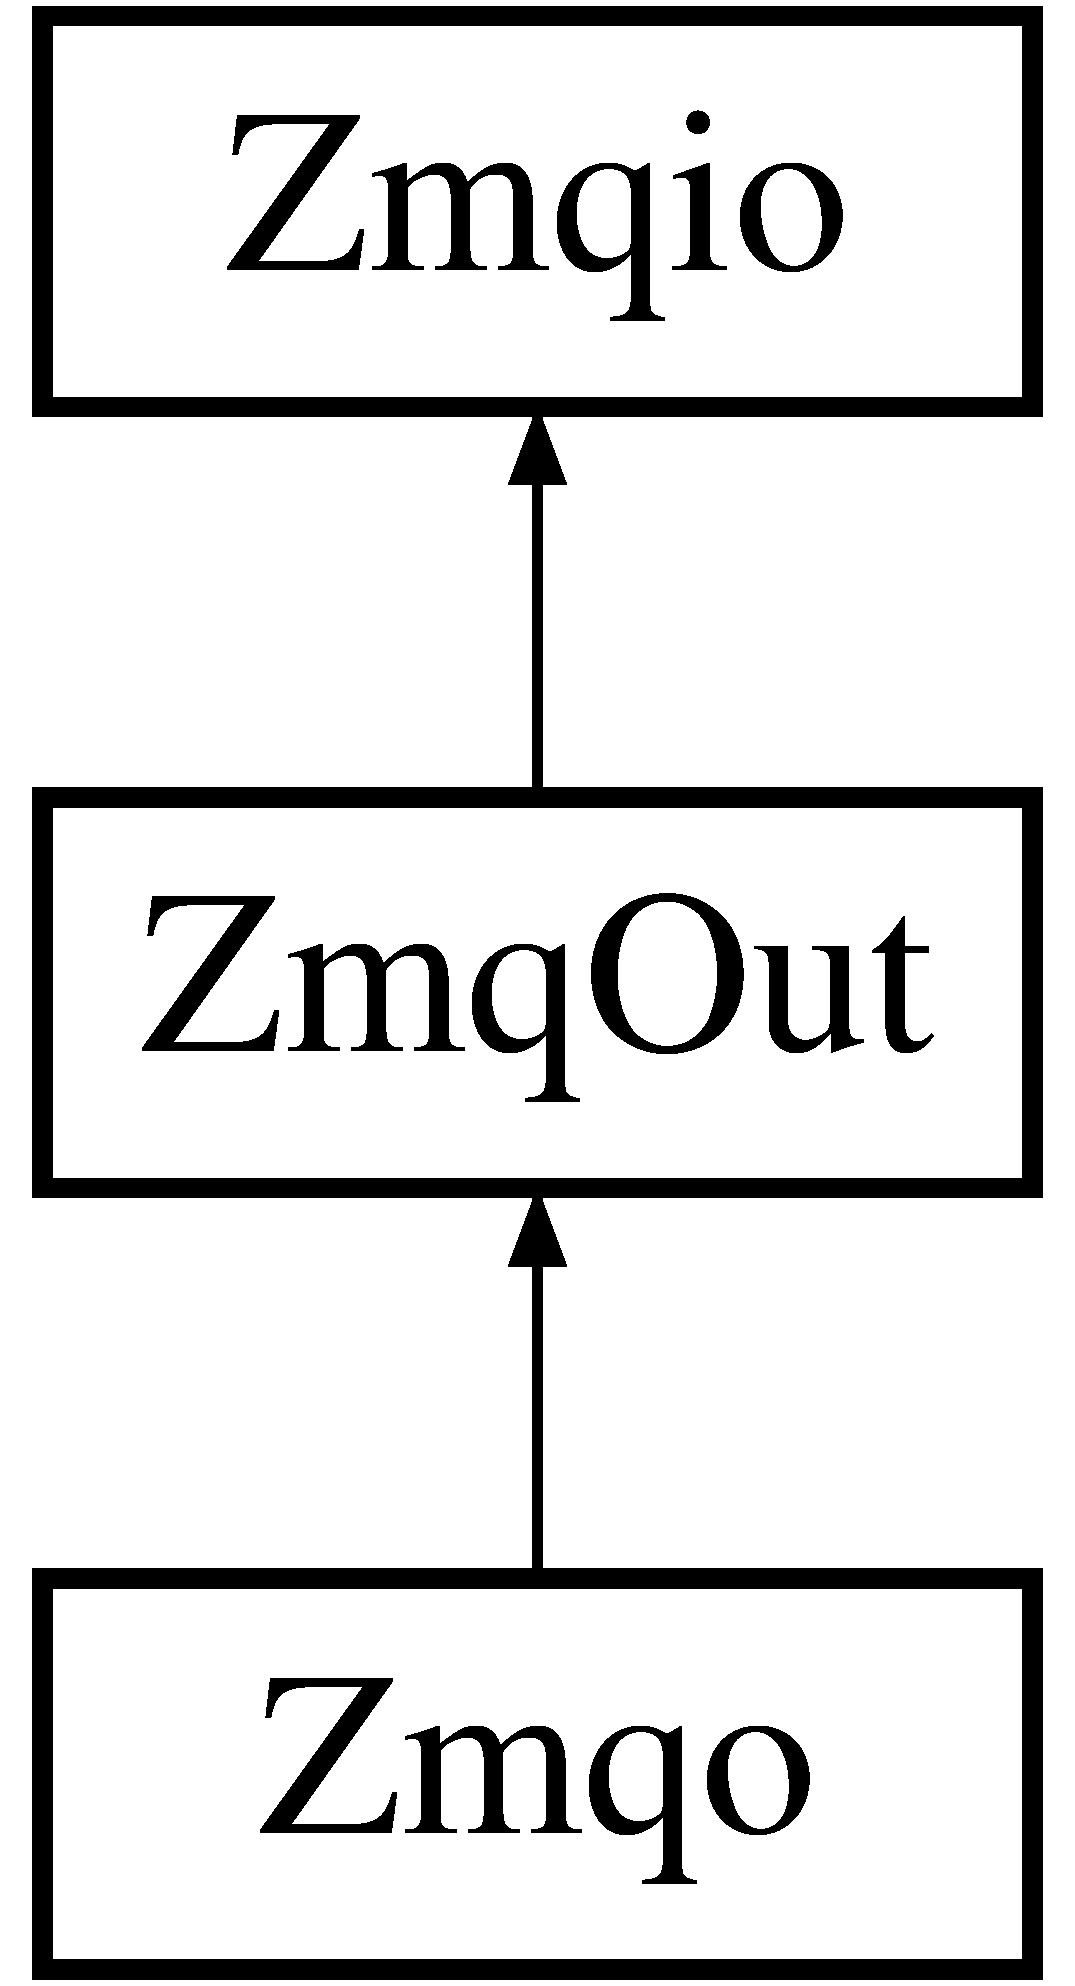
\includegraphics[height=2.000000cm]{classZmqOut}
\end{center}
\end{figure}
\subsection*{Public Member Functions}
\begin{DoxyCompactItemize}
\item 
\hypertarget{classZmqOut_ae34b1742c72e0c82ea42315cb68f1a20}{virtual void \hyperlink{classZmqOut_ae34b1742c72e0c82ea42315cb68f1a20}{connect} (std\-::string conn\-\_\-str)=0}\label{classZmqOut_ae34b1742c72e0c82ea42315cb68f1a20}

\begin{DoxyCompactList}\small\item\em Connect to the given conn\-\_\-str. \end{DoxyCompactList}\item 
\hypertarget{classZmqOut_a97935d9e7cbacd2fcb9655433e4b7af4}{virtual void \hyperlink{classZmqOut_a97935d9e7cbacd2fcb9655433e4b7af4}{send} (const char $\ast$msg, int msg\-\_\-size)=0}\label{classZmqOut_a97935d9e7cbacd2fcb9655433e4b7af4}

\begin{DoxyCompactList}\small\item\em Send a message on the port. \end{DoxyCompactList}\item 
\hypertarget{classZmqOut_ac7b314ddf6e0357c31b05fb2b1b91635}{virtual void \hyperlink{classZmqOut_ac7b314ddf6e0357c31b05fb2b1b91635}{send} (std\-::string msg)=0}\label{classZmqOut_ac7b314ddf6e0357c31b05fb2b1b91635}

\begin{DoxyCompactList}\small\item\em Send a string on the port. \end{DoxyCompactList}\item 
\hypertarget{classZmqOut_a02da5e5dd51f99e7d35a3f843b9bd00e}{virtual std\-::string \hyperlink{classZmqOut_a02da5e5dd51f99e7d35a3f843b9bd00e}{recv} ()=0}\label{classZmqOut_a02da5e5dd51f99e7d35a3f843b9bd00e}

\begin{DoxyCompactList}\small\item\em Recieve a message on the port. \end{DoxyCompactList}\end{DoxyCompactItemize}


\subsection{Detailed Description}
An Outbound Z\-M\-Q Manager. 

Acts as the Requestor (Client) in the Z\-M\-Q Sockets Send, then Recieve 

The documentation for this class was generated from the following file\-:\begin{DoxyCompactItemize}
\item 
lib/include/factory/zmq\-\_\-interface.\-h\end{DoxyCompactItemize}

%--- End generated contents ---

% Index
\newpage
\phantomsection
\addcontentsline{toc}{chapter}{Index}
\printindex

\end{document}
